%%%%%%%%%%%%%%%%%%%%%%%%%%%%%%%%%%%%%%%%%%%%%%%%%%%%%%%%%%%%%%%%%%%%%%%%%%%%%%
% A user guide for dog stability analysis code.
%
% $Id$
%%%%%%%%%%%%%%%%%%%%%%%%%%%%%%%%%%%%%%%%%%%%%%%%%%%%%%%%%%%%%%%%%%%%%%%%%%%%%%
\documentclass[11pt,a4paper]{report}

\usepackage{
graphicx,
natbib,
bm,
amssymb,
amsmath,
amsfonts
}
\usepackage[colorlinks=true,linkcolor=blue,citecolor=blue]{hyperref}

\graphicspath{{./Figs/}}

\setlength{\textheight}              {245mm}
\setlength{\textwidth}               {160mm}
\setlength{\topmargin}               {-20mm}
\setlength{\oddsidemargin}           {0mm}
\setlength{\parindent}               {2.5ex}
\setlength{\leftmargin}              {2.5ex}
\setlength{\bibsep}                  {\parskip}

\renewcommand{\baselinestretch}      {1.0}
\renewcommand{\topfraction}{0.85}
\renewcommand{\bottomfraction}{0.85}
\renewcommand{\textfraction}{0.15}
\renewcommand{\floatpagefraction}{0.7}

\renewcommand{\familydefault}{cmss}

\newcommand\Rey{\mbox{\textit{Re}}}
\newcommand\Str{\mbox{\textit{St}}}
\newcommand\Pra{\mbox{\textit{Pr}}}
\newcommand\Ros{\mbox{\textit{Ro}}}
\newcommand\real{{\mbox{Re}}}
\newcommand\imag{{\mbox{Im}}}
\newcommand\cd{\mathrm{d}}
\newcommand\ce{\mathrm{e}}
\newcommand\cg{\mathrm{g}}
\newcommand\ci{\mathrm{i}}
\newcommand\half{\frac{1}{2}}
\newcommand\thalf{{\textstyle{\half}}}
\newcommand\ol[1]{\overline{#1}}
\newcommand\wh[1]{\widehat{#1}}
\newcommand\wt[1]{\widetilde{#1}}
\newcommand\ob[1]{\overbrace{#1}}
\newcommand\ub[1]{\underbrace{#1}}
\newcommand\Uinf{U_\infty}
\newcommand\Vinf{V_\infty}
\newcommand\Vrel{V_\textrm{rel}}

\newcommand\NavSto{Navier--Stokes}
\newcommand\LNS{linearized \NavSto}
\newcommand\LNSE{\LNS\ equations}
\newcommand\KH{Kelvin--Helmholtz}
\newcommand\Pois{Poiseuille}
\newcommand\Orrsom{Orr--Sommerfeld}
\newcommand\GL{Ginzberg--Landau}
\newcommand\bfs{back\-ward-fac\-ing step}

\newcommand\qp{qua\-si-per\-io\-dic}
\newcommand\cc{complex-conjugate}
\newcommand\oned{one-di\-men\-sion\-al}
\newcommand\twod{two-di\-men\-sion\-al}
\newcommand\threed{three-di\-men\-sion\-al}
\newcommand\twoc{two-com\-po\-nent}
\newcommand\threec{three-com\-po\-nent}
\newcommand\gll{Gauss--Lobatto--Legendre}
\newcommand\SLO{shear-layer oscillation}
\newcommand{\ie}{i.e.\ }
\newcommand{\eg}{e.g.\ }
\newcommand\etal{{\it et al}.}

\newcommand\Ubase{{\bm{U}}}
\newcommand\Pbase{P}

\newcommand\upert{{\bm{u}'}}
\newcommand\ppert{{p}'}

\newcommand\umode{\tilde{\bm{u}}}
\newcommand\pmode{\tilde{p}}

\newcommand\xvec{\bm{x}}
\newcommand\uvec{\bm{u}}
\newcommand\uadj{\bm{u}^*}
\newcommand\qvec{\bm{q}}
\newcommand\qadj{\bm{q}^*}
\newcommand\padj{p^*}

\newcommand\qcs{\tilde{\bm{q}}}
\newcommand\qacs{\tilde{\bm{q}^*}}
\newcommand\qh{\hat{\bm{q}}}
\newcommand\qah{\hat{\bm{q}^*}}

\newcommand\Aop{{\cal A}}
\newcommand\Aadj{{\cal A^*}}
\newcommand\Hop{{\cal H}}
\newcommand\Hadj{{\cal H^*}}
\newcommand\Lop{{L}}
\newcommand\Ladj{{L^*}}
\newcommand\Mop{{\cal M}}
\newcommand\Madj{{\cal M^*}}

\newcommand\DN{\text{DN}}
\newcommand\DNadj{\text{DN}^*}

\newcommand\opt{\textrm{max}}
\newcommand\tauopt{\tau_\opt}
\newcommand\Gmax{G_\opt}

\hyphenation{axi-sym-met-ric}

\newcommand{\Semtex}{\emph{Semtex}}
\newcommand{\Dog}{\emph{Dog}}
\newcommand{\Tecplot}{\emph{Tecplot}}
\newcommand{\Paraview}{\emph{Paraview}}
\newcommand\undertext[1]{\underline{\smash{\hbox{#1}}}}


%%%%%%%%%%%%%%%%%%%%%%%%%%%%%%%%%%%%%%%%%%%%%%%%%%%%%%%%%%%%%%%%%%%%%%%%%%%%%%
% Condensed lists.
%

% -- Bullet.

\newenvironment{conlist}
  {\vspace*{0ex}
    \begin{list}{$\bullet$}%
      {\setlength{\itemsep}{0pt}%
       \setlength{\parsep}{0pt}%
       \setlength{\topsep}{0pt}%
       \setlength{\leftmargin}{12pt}%
      }%
  }%
  {\end{list}}

% -- Open dot.

\newenvironment{conlistd}
  {\vspace*{0ex}
    \begin{list}{$\circ$}%
      {\setlength{\itemsep}{0pt}%
       \setlength{\parsep}{0pt}%
       \setlength{\topsep}{0pt}%
       \setlength{\leftmargin}{12pt}%
      }%
  }%
  {\end{list}}

% -- Numbered.

\newcounter{beann}
\newenvironment{conlistn}
  {\vspace*{0ex}
    \begin{list}{\arabic{beann}.}{%
      \usecounter{beann}%
      \setlength{\parsep}{0pt}%
      \setlength{\itemsep}{0pt}%
      \setlength{\parsep}{0pt}%
      \setlength{\topsep}{3pt}%
      \setlength{\leftmargin}{28pt}%
      \setlength{\labelwidth}{12pt}%
      \setlength{\topskip}{0pt}%
      }%
  }%
  {\end{list}}

% -- Alpha (a) (b) (c)...

\newcounter{beanna}
\newenvironment{conlista}
  {\vspace*{0ex}
    \begin{list}{(\alph{beanna})}{%
      \usecounter{beanna}%
      \setlength{\parsep}{0pt}%
      \setlength{\itemsep}{0pt}%
      \setlength{\parsep}{0pt}%
      \setlength{\topsep}{3pt}%
      \setlength{\leftmargin}{28pt}%
      \setlength{\labelwidth}{12pt}%
      \setlength{\topskip}{0pt}%
      }%
  }%
  {\end{list}}


%%%%%%%%%%%%%%%%%%%%%%%%%%%%%%%%%%%%%%%%%%%%%%%%%%%%%%%%%%%%%%%%%%%%%%%%%%%%%%
\begin{document}

\begin{titlepage}
\centering

\vspace*{\fill}

%{\huge Working \Dog}

\vspace{\fill}

\begin{figure}[h]
\begin{center}
%  \fbox{
\includegraphics[width=0.5\textwidth]{F7585}}
  \includegraphics[width=0.7\textwidth]{A56}
\end{center}
\end{figure}

\vspace{\fill}

{\large H.\,M. Blackburn}\\
Monash University

\vspace{\fill}

\today

\Dog\ version 2.0

\vspace*{\fill}

\end{titlepage}

%%%%%%%%%%%%%%%%%%%%%%%%%%%%%%%%%%%%%%%%%%%%%%%%%%%%%%%%%%%%%%%%%%%%%%%%%%%%%%

\tableofcontents

\clearpage

%%%%%%%%%%%%%%%%%%%%%%%%%%%%%%%%%%%%%%%%%%%%%%%%%%%%%%%%%%%%%%%%%%%%%%%%%%%%%
\chapter{Introduction}

\Dog\ is a tool to compute solutions to stability analysis and/or
optimal transient growth problems in steady or time-periodic
incompressible viscous flows with moderate \twod\ geometric complexity
in either Cartesian or cylindrical coordinates.  Such stability
analyses are sometimes referred to of `global' type in order to
distinguish them from `local' or sectional analyses which were the
previous norm.  The name \Dog\ is an acronym of '\undertext{d}irect
\undertext{o}ptimal \undertext{g}rowth'.
%
In effect \Dog\ provides an iterative eigensystem solution wrapper
around routines which timestep the linearised \NavSto\ equations and
their adjoint.

\Dog\ is built on top of the author's \Semtex\ DNS application, and so
employs quadrilateral nodal spectral elements as the underlying
spatial discretization. It is highly recommended that you have some
familiarity with setting up and running problems in \Semtex\ before
attempting to use \Dog. If you are planning to compile \Dog\ you need
to have a working \Semtex\ installation first\,---\,please see the
setup instructions in the \Semtex\ user guide.  The default location
for the \Dog\ directory is at the same level as where you put the
\Semtex\ directory, though it is also straightforward to install it
within the \Semtex\ directory (edit \verb+dog/Makefile+).

I would very much like to acknowledge the contributions made to this
code, as well as to the ideas in the present document, by Dwight
Barkley (who originally wrote the \texttt{flok} program which was the
prototype for \Dog\ and who, together with Spencer Sherwin, helped
develop the optimal growth tools in \Dog), Ron Henderson (whose DNS
code \texttt{prism} was the underlying basis for \texttt{flok} and
which was also the progenitor of \Semtex), Spencer Sherwin and Xuerui
Mao. I should add that Laurette Tuckerman has also long been a
champion of flow analysis methods based on integration of the
\NavSto\ equations, which is the methodology used by \Dog.  It's been
a great experience to work with all of you.

It seems worth remarking at the outset that global flow stability
analysis, like most iterative solution of large eigensystems, is
somewhat of an art.  Experience, judgement and determination seem to
play a greater role here than is the case for DNS.  If you do succeed
in obtaining converged solutions, it pays not to trust them at first;
examine convergence, find ways to check outcomes.  If you do not
obtain converged eigenvalue estimates at first try, be prepared to
make changes and persist. 

%=============================================================================
\section{\Dog\ and its kin}

These are the codes that can be built with the upper-level Makefile:
\begin{tabbing}
\texttt{symmetrisexx} \= \kill
% 
\texttt{dog} 
\> The central eigensystem code. Computes linear stability analysis or 
optimal \\
\> transient growth for a two-dimensional base flow.\\
%
\texttt{lns} 
\> Integrate the linearised \NavSto\ equations and/or their adjoint\\ 
\> (\eg to evolve an eigenmode or optimal initial condition).\\ 
\> This drives exactly the same routines that \texttt{dog} uses.\\
%
\texttt{normalize} 
\> Normalise an eigenmode or initial condition \\
\> (\eg so it has unit kinetic energy per unit mass).\\
%
\texttt{combine} 
\> Combine a base flow with an eigenmode/IC to
produce an initial condition \\ \> \emph{in physical space} (\eg for
subsequent evolution using \texttt{dns}, part of \Semtex).\\
%
\texttt{circulate} 
\> `Rotate' a sequence of base flows to generate a different starting phase\\ 
\> for Floquet or transient analysis. 
   Made redundant by \verb+T_OFFSET+ token.\\
%
\texttt{flipmap} 
\> Generate a set of mapping indices for a `half-period flip'.\\
%
\texttt{symmetrise} 
\> Enforce a reflection symmetry (from flipmap) on a field file.
\end{tabbing}

There are also a couple of more specialised executables that can be
built: \texttt{dog-H} \citep[for computing stability with a
  half-period flip, see e.g.][]{bml05} and \texttt{dog-AR} which uses
\texttt{ARPACK} \citep{lehoucq98} as the Arnoldi eigensystem solver as
opposed to the (default) `Barkley' method documented in
\citet{bbs08b}.  To make \texttt{dog-AR} after building \texttt{dog}
use these commands: \verb+rm drive.o; make ARPACK=1+.  While it is
useful to be able to use the \texttt{ARPACK} version in some
situations (\eg it can perform better at converging a significant
number of eigenvalues), we generally use the default eigensystem
solver as it provides better diagnostic information.  I suggest you
only try \texttt{dog-AR} on a problem once a converged solution can be
obtained with the default solver.

%============================================================================
\subsection{Files}

Just like \Semtex, \Dog\ needs a starting input file which describes
the mesh, boundary conditions, and sets up tokens used by the solver.
We call this a \verb+session+ file and typically it has no root
extension.  It is written in a format patterned on HTML, which we have
called FEML (for Finite Element Markup Language). An extra input file
required by \Dog\ is \verb+session.bse+ which contains the base
flow. There are a number of example session files in the
\verb+semtex/mesh+ directory.  Other files have standard extensions:
\begin{tabbing}
\texttt{session.bsexxxx} \= \kill 
%
\undertext{\texttt{session.bse}}  \>
        Base flow on which analysis is performed.  Same format as
        \texttt{session.fld}.\\
\undertext{\texttt{session.evl}} \>
        Eigenvalue (and convergence) information.\\
\undertext{\texttt{session.eig.X}} \> Eigenvector \texttt{X}. 
        Same format as \texttt{session.fld}\\
\texttt{session.fld}  \>
        Solution/field file.  Binary format by default.\\
\texttt{session.num}  \>
        Global node numbers, produced by enumerate utility.\\
\undertext{\texttt{session.run}}  \>
        Runtime information including PID, command line arguments, etc.\\
\texttt{session.rst}  \>
        Restart file. Read in to initialize solution if present.\\
\texttt{session.his} \> History point data.\\
\undertext{\texttt{session.bhs}} \> 
       (Reconstructed) base flow history point data 
       if requested in \texttt{BASE\_HIS} section.\\
\texttt{session.mdl} \> Time series of kinetic energy of the perturbation.
\end{tabbing}
(\undertext{Underlined} file names are specific to \Dog.)  The primary
focus when running \Dog\ is usually the \verb+session.evl+ file. It is
good practice to use \verb+tail -f session.evl+ in order to monitor
progress of convergence.


%============================================================================
\subsection{Usage}

{\small
\begin{verbatim}
[mec-aquila]$ dog -h
dog(-H) [options] session
options:
-h       ... print this message
-v       ... set verbose
-a||g||s ... solve adjoint or optimal growth or optimal shrink, problem
-k <num> ... set dimension of subspace (maximum number of pairs) to num
-m <num> ... set maximum number of iterations         (m >= k)
-n <num> ... compute num eigenvalue/eigenvector pairs (n <= k)
-t <num> ... set eigenvalue tolerance to num [Default 1e-6]
-p       ... compute pressure from converged velocity eigenvector
\end{verbatim}
}
NB: the eigenvalue or growth tolerance (set using \verb+-t+) is
scaled by the corresponding \verb+MAGNITUDE+.  So if the leading
eigenvalue (or the last one requested) has magnitude 0.5 and the
tolerance is $1\times10^{-6}$, convergence won't be deemed to be
achieved until the corresponding residual falls below
$0.5\times1\times10^{-6}=5\times10^{-7}$.

{\small
\begin{verbatim}
[mec-aquila]$  lns -h
Usage: lns [options] session-file
[options]:
-h        ... print this message
-a        ... use adjoint LNSE instead of primal LNSE
-i[i]     ... use iterative solver for viscous [& pressure] steps
-v[v...]  ... increase verbosity level
-chk      ... checkpoint field dumps
\end{verbatim}
}

{\small
\begin{verbatim}
[mec-aquila]$ normalize
ERROR: normalize: Usage: normalize [options] session [session.fld]
options:
-h       ... print this message
-p       ... mode normalization on pressure rather than velocity
-s scale ... multiplicative scale applied after normalization
\end{verbatim}
}

{\small
\begin{verbatim}
[mec-aquila]$ combine -h
Usage: combine [options] base pert
options:
-h       ... print this message.
-b <num> ... set beta, wavenumber of base flow to <num> (3D) [Default: 1.0]
-r <num> ... relative energy of perturbation is <num>.       [Default: 1.0]
-s       ... simple scaling: scaling is pointwise rather than energy-based
-m <num> ... mode number for perturbation is <num> (3D only) [Default: 1]
\end{verbatim}
}

{\small
\begin{verbatim}
[mec-aquila]$ circulate -h
usage: circulate n file
\end{verbatim}
}

{\small
\begin{verbatim}
[mec-aquila]$ flipmap -h
Usage: flipmap [-h] -x || -y || -d [-t <num>] [meshfile]
\end{verbatim}
}

{\small
\begin{verbatim}
[mec-aquila]$ symmetrise
Usage: symmetrise [options] -m mapfile [file]
options:
-h       ... print this message
\end{verbatim}
}

In cases where you are unsure of the purpose of these utiities, we
encourage you to read the headers of their respective source files.

%============================================================================
\subsection{Dimensionality vs componentality}

By `dimensionality' we mean the number of dimensions required to
describe a flow's variation in space whereas by `componentality' we
mean the number of velocity components required to represent it.  We
can use a convenient set of acronyms such as 2D2C, 2D3C, 3D3C.  A very
typical combination is that the base flow will be 2D2C while the
linear stability modes are 3D3C.  The combinations \Dog\ can accept
(base/stability) are: 1D2C/2D2C, 1D2C/2D3C, 2D2C/2D2C, 2D2C/2D3C,
2D3C/2D3C, but is presently not capable of dealing with 3D3C/3D3C.
The coordinate systems available (as for \Semtex) are Cartesian and
cylindrical.  \citep[One might anticipate that 1D2C/2D3C analyses are
  not very useful owing to Squire's theorem for stability of `parallel
  shear flows', see e.g.][but Squire's theorem does not hold in
  cylindrical coordinates.]{schmid01}

%============================================================================
\subsection{\Dog-specific \texttt{TOKENS} and session file sections}
\label{sec.specific}

\begin{tabbing}
\texttt{XXXXXXXXXXXXXX} \= \kill 
%
\texttt{N\_BASE}  \>
  Number of velocity components in 2D base flow file.  Either 2 or 3.\\
\texttt{N\_SLICE}  \>
  Number of `time slices' in base flow file. \verb+N_SLICE=1+ for 
  steady base flow.\\
  \> For periodic base flow, a number with prime factors 2, 3, 5 for FFT.\\
\texttt{BASE\_PERIOD}  \>
  Optional value to declare period of a periodic base flow;\\
  \>  otherwise this value is computed from \verb+session.bse+.\\
\texttt{T\_OFFSET}  \>
  Optional value to declare a time offset for reconstruction of base flow;\\
  \>  used to vary phase of Floquet analysis, or initiation time for
      transient growth.\\
\texttt{LAGRANGE\_INT} \>
  Set \verb+LAGRANGE_INT=1+ for cubic Lagrange interpolation of base flow.\\
  \> Leave unset/0 for default Fourier interpolation.\\
\texttt{BIG\_RESIDS} \>
  Set \verb+BIG_RESIDS=1+ to force direct computation of 
  eigenvector residuals.
\end{tabbing}

An optional section of the session file is \verb+BASE_HIST+, which may
be used to check the temporal regeneration of a base flow from a
limited number of time slices.  This is similar in concept and
structure to a \verb+HISTORY+ section in a standard \Semtex\ session
file. It calls up output of history point data from the
periodic/unsteady base flow reconstruction into file
\verb+session.bhs+, with contents similar to those in
\verb+session.his+, but lacking pressure history.  Output generated
every \verb+IO_HIS+ steps.

%============================================================================
\subsection{`Throw the first one away'}

A feature you may notice when running \verb+dog+ is that with the
default starting condition (no \verb+.rst+ file), the first iteration
of time-integration over interval $\tau$ seems to produce no result in
the upper-level monitor file \verb+session.evl+.  This is because the
default starting condition is pseudo-random white noise\,---\, which
produces velocity files with non-zero divergence.  If convergence
occurs before the Krylov sequence is filled, the resulting Ritz
estimates of eigenvectors may be corrupt.  A simple work-around is to
ignore the first iteration.

%%%%%%%%%%%%%%%%%%%%%%%%%%%%%%%%%%%%%%%%%%%%%%%%%%%%%%%%%%%%%%%%%%%%%%%%%%%%%%
\chapter{Theory}
\label{ch.theory}

This chapter contains sufficient depth to be able to understand and
use \Dog, but is by no means a full treatment of the theory on which
flow stability analysis is based.  It is assumed that the reader has
previously taken a course that deals with eigensystem analysis of
linear systems.
%
The standard text in the general area of flow stability analysis is
\citet{schmid01} although it tends to concentrate on analysis of
\oned\ flows via the \Orrsom\ equations.
%
A good introductory reference for the timestepper-based methods
advanced in this chapter is \citet{tuba00}.
%
For stability analysis of \twod\ steady flow, \citet{bgh02} is a good
starting point; for stability analysis of time-periodic flow,
\cite{bah96} is required reading; a good introduction to transient
growth analysis is provided by \citet{bbs08a}, while \citet{bbs08b}
provides a more detailed explanation of the underlying mathematics of
transient growth analysis and includes a description of the
eigensystem solution method that is standard in \Dog.

%=============================================================================
\section{The \LNSE\ in operator form}

We start with the incompressible \NavSto\ equations
\begin{equation}
\partial_t\uvec=-\uvec\bm{\cdot \nabla}\uvec -\bm{\nabla} p
+\Rey^{-1}\nabla^2 \uvec, \quad \text{with} \quad\bm{\nabla\cdot}\uvec=0,
\end{equation}
where $p$ is the modified or kinematic pressure, $\uvec$ is the
velocity vector, while the Reynolds number $\Rey=UD/\nu$ where $U$ and
$D$ are convenient velocity and length scales and $\nu$ is kinematic
viscosity. 
%
Decomposing the flow field as the sum of a base flow and a
perturbation \ie $(\uvec,p)=(\Ubase,P)+(\upert,\ppert)$ we first substitute
\begin{equation}
\partial_t(\Ubase+\upert) = -(\Ubase+\upert)\bm{\cdot\nabla}(\Ubase+\upert)
  - \bm{\nabla}(\Pbase+\ppert)
  + \Rey^{-1}\nabla^2(\Ubase+\upert),
\end{equation}
expand
\begin{equation}
\partial_t(\Ubase+\upert) =
-\Ubase\bm{\cdot\nabla}\Ubase
-\Ubase\bm{\cdot\nabla}\upert
-\upert\bm{\cdot\nabla}\Ubase
-\upert\bm{\cdot\nabla}\upert
- \bm{\nabla}(\Pbase+\ppert)  
+ \Rey^{-1}\nabla^2(\Ubase+\upert), 
\end{equation}
then collect into equations for evolution of the base flow
\begin{equation}
\partial_t\Ubase =
-\Ubase\bm{\cdot\nabla}\Ubase
- \bm{\nabla}\Pbase
+ \Rey^{-1}\nabla^2\Ubase,
\end{equation}
and perturbation
\begin{equation}
\partial_t\upert =
-\Ubase\bm{\cdot\nabla}\upert
-\upert\bm{\cdot\nabla}\Ubase
-\upert\bm{\cdot\nabla}\upert
- \bm{\nabla}\ppert
+ \Rey^{-1}\nabla^2\upert,
\end{equation}
from which we omit interaction of perturbations (assuming those terms
to be $O(\upert^2)$), to obtain the \LNSE, which
govern the evolution of infinitesimal perturbations, as
\begin{equation}
\partial_t\upert
=-[\bm{U \cdot\nabla}+(\bm{\nabla U})^T\bm{\cdot}] \upert 
-\bm{\nabla} \ppert+\Rey^{-1}\nabla^2 \upert.
\label{eq.LNS} 				
\end{equation}

We note that the base flow $\Ubase$ does not have to be steady in
time: it may also be time-periodic, or have more general structure.

Considering that in incompressible flow the pressure may be considered
a constraint field whose gradient keeps the flow divergence-free and
which is obtained from the advection terms as the solution of a
Poisson equation, we can symbolically state that
\begin{equation}
\ppert\equiv
\nabla^{-2}\bm{\nabla\cdot}\left[\Ubase\bm{\cdot\nabla}
+(\bm{\nabla\Ubase})^\text{T}\bm{\cdot}\right]\upert
\end{equation}
and so we can write the \LNS\ symbolically without the pressure term as
\begin{equation}
\partial_t\upert =
-\left[\bm{I}-\bm{\nabla}\nabla^{-2}\bm{\nabla\cdot}\right]
\left[\Ubase\bm{\cdot\nabla}
  +(\bm{\nabla\Ubase})^\text{T}\bm{\cdot}\right]\upert
+ \Rey^{-1}\nabla^2\upert,
\end{equation}
or more compactly, since now the spatial terms are now just a linear
operator applied to the perturbation velocity, we write the
\LNS\ equations in operator form as
\begin{equation}
\partial_t\upert-\Lop(\upert)=0.		
\label{eq.lns}
\end{equation}
The above notation is adopted largely for compactness/convenience and
does not imply that the pressure is not computed.  However, it is
typically only the velocity components which are considered as part of
the numerical eigensystem analysis of incompressible flows.

Before proceeding to consider stability analysis, it should be noted
that since the base flow $\Ubase$ is required as input, one must pay
considerable attention to obtaining a good estimate for it.  In fact,
this precursor requirement often consumes a substantial part of the
overall effort in performing a stability analysis.  Fortunately
however, one can very often re-use the session files used for
computing the base flow as a starting point for those employed in
stability analysis (typically one must change the boundary conditions
and a few other minor things).

As a side-note, \citet{wikl01} showed that for the $P_N$--$P_{N-2}$
spectral element formulation of the discretized incompressible
\NavSto\ equations, both the conservative ($\bm{\nabla\cdot uu}$) and
skew-symmetric ($(\bm{\nabla\cdot uu}+\bm{u\cdot\nabla u})/2)$ forms
of the nonlinear terms possess a linear instability, while the
non-conservative form $\bm{u\cdot\nabla u}$ does not.  While it is
standard/default for \Semtex/\verb+dns+ (which is $P_N$--$P_N$) to
employ the (alternating) skew-symmetric form of the nonlinear terms
for robustness, we have found that carrying this form over to the
discretized \LNS\ equations causes spurious predictions of
instability, in apparent agreement with \citeauthor{wikl01}'s
finding. Hence the implementation of the linearized advection terms
used by \verb+dog+ and \verb+lns+ uses the non-conservative form, just
as written in \eqref{eq.LNS}.

%=============================================================================
\section{Timestepping, the exponential mapping, and eigensystems}
\label{sec.timestep}

So now let us consider the effect of evolving (time-integrating,
timestepping) a perturbation $\upert$ from an initial state at (let's
say) $t=0$ over a time interval (period, horizon) $\tau$.
\begin{equation}
\upert_\tau=\Mop(\tau)\upert_0
\label{eq.STO}
\end{equation}
where 
\begin{equation}
\Mop(\tau) = \exp \int_{t=0}^{t=\tau}\Lop(t)\,\cd t
\end{equation}
is the state transition operator of the \LNSE. We note that
\eqref{eq.STO} is symbolic shorthand for `apply the \LNS\ equations to
an initial condition by time-integration over interval $\tau$' and is
what we approximate when running a simulation code that evolves our
numerical approximation to the \LNSE. Conceptually this is a
forwards-in-time mapping which we illustrate in
figure~\ref{fig.forwards}. It is also important to note that in
carrying out this numerical integration the time interval $\tau$ is
typically broken into a large number of time steps $\Delta t$.
%
\begin{figure}
\begin{center}
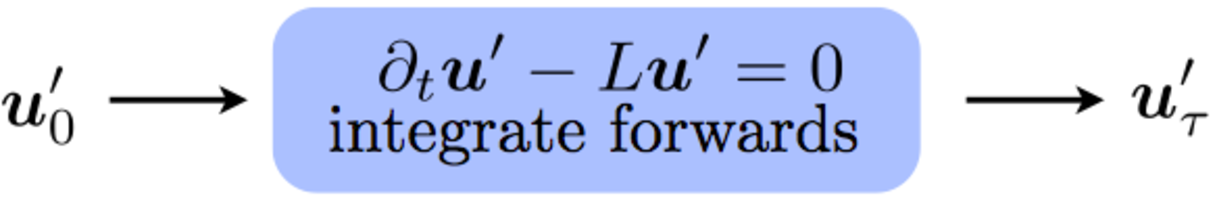
\includegraphics[width=0.4\textwidth]{forwards}
\end{center}
\caption{Applying the timestepping operator $\Mop(\tau)$ to evolve an
  initial condition to a later time.}
\label{fig.forwards}
\end{figure}

If $\Ubase$ is steady in time, then so is $\Lop$, in which case $\Mop$
has a particularly simple written form
\begin{equation}
\Mop(\tau)=\exp(\Lop\tau).
\label{eq.map}
\end{equation}

%-----------------------------------------------------------------------------
\subsection{Linear stability analysis of steady flows}
\label{sec.steady}

We now turn to the problem of finding the eigensystem of $\Lop$ or
equivalently of $\Mop(\tau)$ in the case where the base flow $\Ubase$
is steady in time.  Assuming a separation-of-variables form for the
growth of a linear perturbation, viz.,
$\upert(\xvec,t)=\exp(\lambda_jt)\wt{\bm{u}}_j(\xvec)$, substitution
into \eqref{eq.lns} produces
\begin{equation}
\Lop \wt{\bm{u}}_j = \lambda_j \wt{\bm{u}}_j,
\label{eq.eig}
\end{equation}
\ie an eigenvalue problem for the the set of eigenvalues $\lambda_j$
and eigenvectors (or `mode shapes') $\wt{\bm{u}}_j(\xvec)$ of the
operator $\Lop$.  Collectively, the eigenvalues and eigenvectors are
called the eigensystem of $\Lop$, and its properties govern the
large-time or asymptotic behaviour of $\upert$.\footnote{We will deal
  with the finite-time behaviour in \S\,\ref{sec.optimal}.} The
reconstruction of $\upert$ from the eigensystem is
\begin{equation}
\upert(\xvec, t) = \sum_{j=0}^\infty
\exp(\lambda_j t)\wt{\bm{u}}_j(\xvec) +\text{c.c.}
\label{eq.sep}
\end{equation}
where we will consider that the eigenvalues may be complex
($\lambda=\lambda_r\pm\ci\lambda_i$) but the eigenvectors are real. The
set of all the eigenvalues of an operator is called its spectrum. We
note that (as is sometimes reversed in textbooks) $\lambda_r$ is a
growth rate and $\lambda_i$ is a (circular) frequency.  We also note
that \eqref{eq.eig} is generated directly by substituting the
separation-of-variables form \eqref{eq.sep} into \eqref{eq.lns}. A
linear stability analysis of a \NavSto\ problem amounts to finding the
leading (least stable) eigenvalues of $\Lop$ and the corresponding
mode shapes (perturbation flows).

Now, for simple flows (\eg \oned\ base flows), we may be able to
afford to explicitly construct a matrix approximation for the operator
$\Lop$ and find its full eigensystem directly \citep[see \eg appendix
  A of][]{schmid01}. However, for more complicated flows a direct
solution may be very expensive computationally (in both time and
memory) and we typically have to resort to matrix-free iterative
methods.  Iterative eigensystem solvers of the Arnoldi type
\citep{saad92} rely on repeatedly applying an operator (matrix) to a
vector, as in \eqref{eq.STO}, without necessarily explicitly
constructing the operator itself. Such methods are typically best at
converging those eigenpairs which have eigenvalues of largest
magnitude, \ie the part of the spectrum furthest from the origin in
the complex plane.  Also, for stability problems we are usually mostly
concerned with the eigenvalues $\lambda_j$ with largest real part (\ie
the least stable eigenvalues) and do not much care about more stable
modes. By happy coincidence the exponential mapping \eqref{eq.map} has
precisely the feature of transforming the spectrum in such a way that
the least-stable eigenvalues of $\Lop$ become the largest-magnitude
eigenvalues of $\Mop$, as indicated in figure~\ref{fig.map}.  This
means that timestepper-based methods for evolving the \LNSE\ are very
well matched to iterative methods for finding (the leading part of)
the eigensystem of an operator.

\begin{figure}
\begin{center}
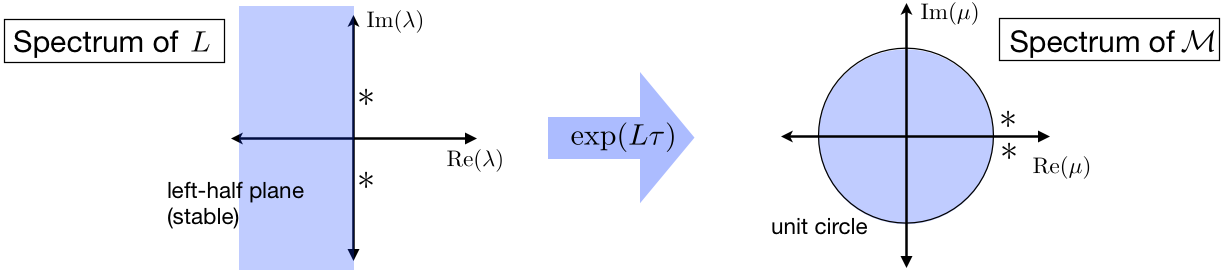
\includegraphics[width=\textwidth]{mapping}
\end{center}
\caption{The timestepper mapping. Left left-half plane of $\Lop$ is
  mapped to inside the unit circle of $\Mop$, and there is a
  one-to-one mapping of the spectrum of the two operators.}
\label{fig.map}
\end{figure}

The eigensystems of $\Lop$ and $\Mop$ are connected.  Since
\begin{equation}
\exp \Lop\tau =
\lim_{N\to\infty}
\sum_{k=0}^{N}
\frac{\left(\Lop\tau\right)^k}{k!}
\end{equation}
we find that the eigenvectors of $\Lop$ are the same as those of
$\Mop(\tau)$: supposing $\wt{\bm{u}}_j$ is an eigenvector of $\Lop$ with
corresponding eigenvalue $\lambda_j$.  Then
\begin{equation}
\Mop\wt{\bm{u}}_j=
\exp \Lop\tau\,\wt{\bm{u}}_j=
\lim_{N\to\infty}\sum_{k=0}^N\frac{\left(\Lop\tau\right)^k}{k!}\wt{\bm{u}}_j=
\lim_{N\to\infty}\sum_{k=0}^N\frac{\left(\lambda_j \tau\right)^k}{k!}\wt{\bm{u}}_j=
\exp(\lambda_j\tau)\wt{\bm{u}}_j,
\end{equation}
\ie $\wt{\bm{u}}_j$ is also an eigenvector of $\Mop(\tau)$, with
corresponding mapped eigenvalue $\mu_j=\exp(\lambda_j\tau)$.  In fact,
since we will be finding the (complex) eigenvalues
$\mu_j=\sigma_{r,j}\pm\ci\sigma_{i,j}$ of $\Mop(\tau)$, we note that
their polar magnitudes and angles in the complex plane are given by
\begin{equation}
|\mu_j|=(\sigma_{r,j}^2+\sigma_{i,j}^2)^{1/2},\qquad
\angle\mu_j=\pm\arctan(\sigma_{i,j}/\sigma_{r,j})
\end{equation}
(using the `two-argument' $\arctan$ function).  From these values we
can work back to find the real and imaginary parts of the eigenvalues
$\lambda_j$ of $\Lop$:
\begin{equation}
\lambda_{r,j}=\ln(|\mu_j|)/\tau,\qquad
\lambda_{i,j}=(\angle\mu_j)/\tau.
\label{eq.convert}
\end{equation}

The base flow is (linearly) neutrally stable when the largest
$|u_j|=1$ or equivalently when the least stable mode has
$\lambda_{r,j}=0$.  Finding the parameter(s) which results in neutral
stability is usually the primary focus of a flow stability
analysis. This value is typically referred to as the `critical' value,
\eg critical Reynolds number $\Rey_c$.

So far we have not touched on the spatial structure of the linear
perturbations $\upert$ or the eigenmodes $\wt{\upert}$. Since the
analysis is linear, we can apply other linear operators to the
methodology without breaking its validity. As the domains we can
consider with \Semtex\ are \twod\ it is natural (if both the geometry
and base flow are \twod) to use a \oned\ Fourier transform in the
out-of-plane/spanwise/homogeneous ($z$) direction to be able to tackle
\threed\ analyses.  Owing to the linearity of both the Fourier
transform and the \LNS\ equations, we can consider the stability of
each \threed\ Fourier mode individually.  While the base flows must be
\twod\, they can be either \twoc\ or \threec.

The definition of the (\oned) Fourier transform employed in
\Semtex\ and \Dog\ is
\begin{align}
\wh{\bm{u}}_k(x,y,t) &=
L_z^{-1}\int_0^{L_z}\bm{u}(x,y,z,t)\ce^{-\ci(2\pi/L_z)kz}\,\cd z,\\
\bm{u}(x,y,z,t) &= 
\sum_{k=-\infty}^\infty\wh{\bm{u}}_k(x,y,t)\ce^{\ci(2\pi/L_z)kz},
\end{align}
where $k$ is an integer mode index and $L_z$ is an assumed periodic
length of the domain in the $z$ direction.  Interchangeably we can take
the spanwise wavenumber $\beta=2\pi/L_z$ (and this is the meaning of
the token \verb+BETA+).  Since for \Dog\ we restrict the base flows to
be \twod\, we can just consider the Fourier transform of the
\LNS\ equations to be taken, and $\upert$ to be a \twod\ complex
mode\,---\,and since we then deal with modes one at a time we can
assume $k=1$ without loss of generality.  The form of the
\LNS\ equations in coordinate-free notation (as we have used above) is
unaltered, but with the understanding that $\Ubase(x,y)$ is \twod\ and
real, while $\upert(x,y)$ is a \twod\ complex mode when $\beta\ne0$.
Within \Dog, any time where we would have a $\partial(\,)/\partial_z$
operation in physical space it is replaced with an $\ci\beta(\,)$
operation on a complex mode, while $\partial^2(\,)/\partial_z^2$ is
replaced with $-\beta^2(\,)$ ($x$ and $y$ derivatives are unaltered
since we only transformed in $z$).

As pointed out by \citet{bah96} a very useful simplification in the
structure of the \twod\ complex Fourier mode $\wh{\uvec}$ occurs if
$\Ubase$ is 2D2C.  In that case, a mode of the form
\begin{align}
(u', v', w') & =
  (\hat{u}\cos\beta z, \hat{v}\cos\beta z, -\hat{w}\sin\beta z),\\
p'         & = 
   \hat{p}\cos\beta z
\end{align}
will pass through the \LNS\ equations with the same form, thus
satisfying essential conditions for an eigenmode.  The form
corresponds to a `half complex' mode, where only the real parts of
$\hat{u}, \hat{v}, \hat{p}$ and the imaginary part of $\hat{w}$ need
be populated.  We can use \verb+N_Z=1+ in the sesssion file for
stability analysis and time integration requires only half the
computational work of a fully-populated complex mode.  The form
embodies a fixed spatial phase relationship along the $z$ axis, but
any arbitrary phase shift (rotation) is equally valid, too.  If
however, the base flow is 2D3C, then a fully complex mode is required
for $\wh{\uvec}$ (and again any phase shift in the $z$ direction is a
valid mode shape); in these cases we use \verb+N_Z=2+ in our session file.

%-----------------------------------------------------------------------------
\subsection{Boundary conditions for stability analysis}
\label{sec.bcs}

A key consideration in setting boundary conditions for stability
analysis is that boundary conditions may differ for computation of
base flow and perturbation.  If the base flow is driven by boundary
conditions (\eg by an inflow boundary or a moving wall) then the
relevant Dirichlet velocity boundary condition is set in the base flow
computation while the corresponding velocity boundary for the
perturbation would be $\upert=0$.  On a non-moving wall boundary, the
velocity boundary condtions for both base flow and perturbation are
non-slip.  On an outflow boundary, both the base flow and pertubation
will have the same approximation to a stress-free condition. On
periodic boundaries, both the base flow and perturbation will be set
periodic.  Thus the perturbed flow $\bm{u}=\bm{U}+\upert$ satifies the
same boundary conditions as for the underlying \NavSto\ problem.  See
\citet{bah96} for more discussion. We will consider examples in
chapter~\ref{ch.stab}.


We note that consideration of boundary conditions for transient growth
analysis is somewhat different\,---\,generally, the velocity boundary
condition on the perturbation is set to zero on all boundaries, with
the idea that for an open-domain problem the analyst ensures that the
domain is large enough that the perturbation is effectively contained
within it for all time horizons considered. See \S\,\ref{sec.tgbcs}.

%-----------------------------------------------------------------------------
\subsection{Linear stability analysis of time-periodic 
flows\,---\,Floquet analysis}
\label{sec.floquet}

If $\Ubase$ is time-periodic, then so is the operator $\Lop$ and we
carry out temporal Floquet stability analysis \citep[analysis of a
  linear system of ODE/PDE where the coefficients are time-periodic,
  see e.g.][]{iooss90}. In this case, we are typically interested in
how much a disturbance grows from one period of the base flow to the
next.  The method of analysis is in fact very similar to that
described above for steady base flows, but now the time integration
period $\tau$, essentially a choice of the analyst in steady flows, is
fixed to match the period of the base flow, while the eigenmodes are
also time-dependent (and time-periodic).  In this case
\begin{equation}
\upert(\xvec, t+\tau) = \sum_{j=0}^\infty
\mu_j\wt{\bm{u}}_j(\xvec,t\,\textrm{mod}\,\tau) +\text{c.c.}
\label{eq.flok}
\end{equation}
Note the general similarity to \eqref{eq.sep}, but that the
eigenvectors (or Floquet modes) are now time-periodic.  The
eigenvalues $\mu_j$ are referred to a Floquet multipliers.  Since the
analysis now has a distinct `digital' aspect (performed on a
$\tau$-periodic basis) it now only really makes much sense to consider
dealing directly with the timestepper mapping \eqref{eq.STO} and only
be concerned with the right side of figure~\ref{fig.map}.  The Floquet
multipliers say how much a mode grows or shrinks over a period: if
they lie outside the unit circle, the mode grows; if inside, it
shrinks.  A good general reference on global Floquet analysis is the
classic paper by \citet{bah96}.  If the multiplier $\mu=-1$, the
instability is of period-doubling or subharmonic type; if it has
non-zero imaginary part (occurs in complex conjugate pairs) the
instability is \qp\ \citep{bllo03b}.

The base flow for Floquet analysis is provided as a set of time-slices
equi-spaced over $\tau$, and Fourier reconstruction is the typical
means of re-estimating the base flow at any point in its period.  We
note that if the base flow has features which are very sharp in time
(as observable in velocity time-history plots), a considerable number
of time-slices may be needed for accurate reconstruction, and then
Fourier reconstruction may become very costly; in this case a local
cubic spline reconstruction may be used instead, since the
interpolation cost is lower \citep[][set \texttt{LAGRANGE\_INT=1} to
  obtain this functionality]{msb11}.
\footnote{It is also possible to carry along computation of the base
  flow as a separate operation in parallel, an approach sometimes
  adopted in other codes.}

As mentioned above, the Floquet modes are time-periodic, although the
multiplier associated with each mode is a fixed scalar.  A single
Floquet analysis generally only returns the mode (or modes, if more
than one is requested) at one particular phase, the starting phase of
the base flow. If one requires the modes at another phase point, one
can either rotate the order of the base flows (using \Dog's
\verb+circulate+ utility), or ask for a time-shift (use token
\verb+T_OFFSET+).

If the time-periodic base flow occurs as an autonomous limit-cycle
oscillation, then a Floquet analysis in the same subspace as the
original flow (\eg both base flow and Floquet modes are 2D2C) should
have a leading multiplier $\mu=1$.  This corresponds to a neutrally
stable mode that is `tangent' to the limit cycle at each point in its
orbit \citep{iooss90}.  At each point in the cycle, the corresponding
Floquet mode shape should appear the same as the local acceleration
field of the base flow, $\partial \Ubase/\partial t$.  This fact can
sometimes be useful in checking numerical Floquet analysis \citep[see
  e.g.][who approached 2D2C in the limit as $\beta\to0$ and found
  $\mu\to1$ over a range of $\Rey$]{bah96}.  Such a mode only exists
if the base flow is an autonomous limit cycle; it should not exist if
the base flow is driven by time-periodic boundary conditions.

%==============================================================================
\section{Optimal growth of perturbations}
\label{sec.optimal}

The motivation for understanding optimal non-normal growth of
perturbations is that if linear non-normal growth is large enough,
non-linear mechanisms may take over and produce a transition to
turbulence even if the flow is linearly stable in the long term
\citep[see e.g.][]{srk02}.
%
The standard introductory text of this area is \citet{schmid01}. As
far as the application of the concepts to general flows is concerned,
we recommend the article by \citet{bbs08b}.

Since the \LNSE\ are non-symmetric (the operator written in on a
comp\-on\-ent-by-component matrix form is non-symmetric about the
leading diagonal), its eigenmodes are in general `non-normal', meaning
that the energy inner products of distinct modes may be non-zero (\ie
the modes are non-orthogonal or non-normal).  This is different from,
say, the eigenmodes of a spring--mass system, which does have this
property, leading to the ability to examine energetics on a
mode-by-mode basis which is a considerable simplification.  In simple
terms, non-normality of the eigenmodes manifests as their being
visually rather similar or having significant spatial overlap
\citep[see e.g.][]{kibe07}.

In order to examine these issues and to consider the growth of
perturbations, we need to introduce energy-type integrals.
%
Flow is considered within a spatial domain $\Omega$ which has a
boundary surface $\partial\Omega$ and unit outward normal $\bm{n}$, as
indicated in figure~\ref{fig.domain}.  Flow is taken to evolve over
the time interval $[0,\tau]$, so the space-time domain considered is
$\Omega\times[0,\tau]$.

\begin{figure}
\begin{center}
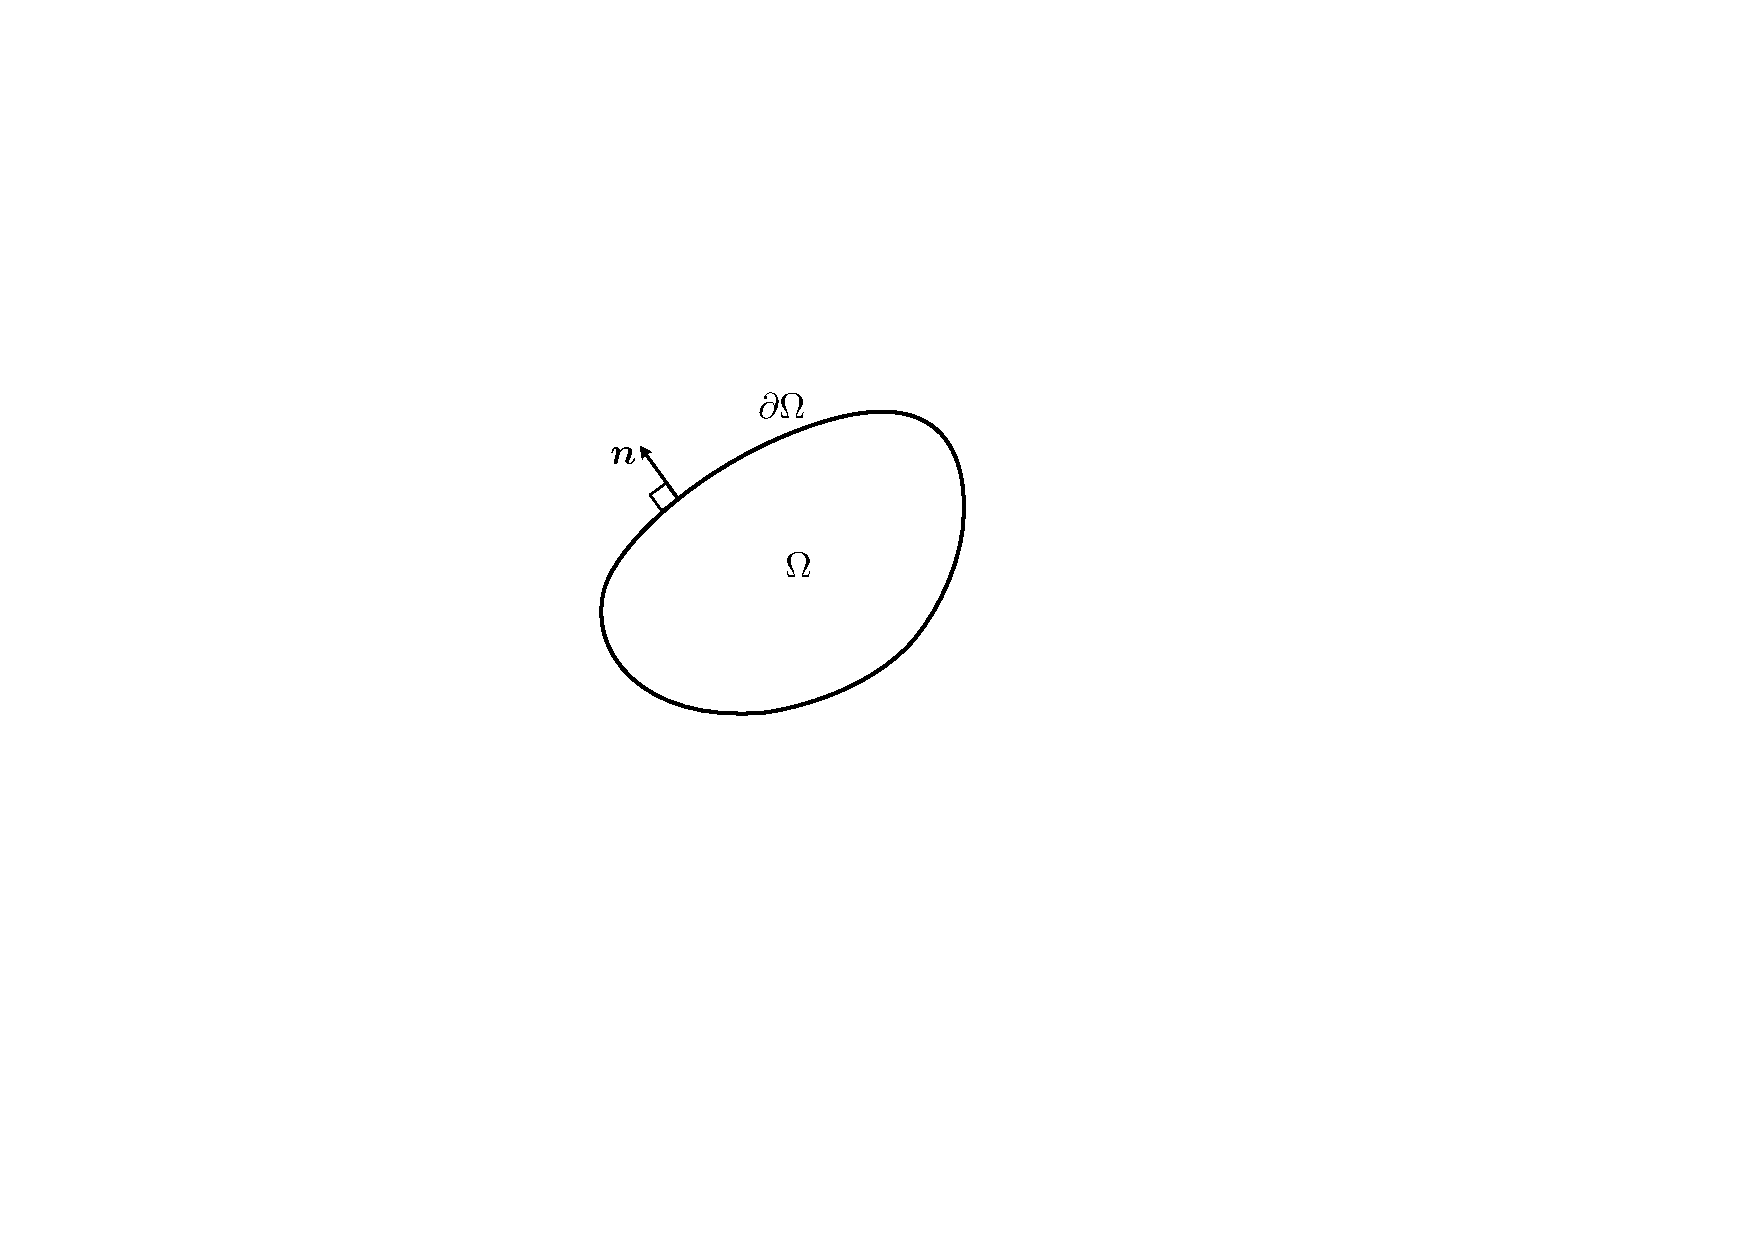
\includegraphics[width=0.25\textwidth]{generaldomain}
\end{center}
\caption{Schematic representation of a spatial flow domain $\Omega$,
  boundary $\partial\Omega$ and unit outward normal vector $\bm{n}$.}
\label{fig.domain}
\end{figure}

The energy inner product of two real modes on domain $\Omega$ can be
written as
\begin{equation}
E=(\wt{\bm{u}}_i, \wt{\bm{u}}_j) = \int_\Omega \wt{\bm{u}}_i
  (\xvec)\bm{\cdot} \wt{\bm{u}}_j(\xvec)\,\cd V.
\label{eq.inner}
\end{equation}
If the modes are orthogonal (and suitably normalised) then
$(\wt{\bm{u}}_i, \wt{\bm{u}}_j)=\delta_{i,j}$ where $\delta_{i,j}$ is
the Kronecker delta, in which case
\begin{align}
\nonumber (\upert,\upert)(t)&=
\int_\Omega\left(\sum_{i=1}^N\exp(\lambda_i t)
\wt{\uvec}_i\right)\bm{\cdot} \left(\sum_{j=1}^N\exp(\lambda_j^\ast
t)\wt{\uvec}_j\right)\,\cd V\\ \nonumber &
=\sum_{i=1}^N\sum_{j=1}^N \exp(\lambda_i t)\exp(\lambda_j^\ast t)
\int_\Omega\wt{\uvec}_i\bm{\cdot}\wt{\uvec}_j\,\cd
V\\ &=\sum_{i=1}^N\exp(2\,\text{Re}(\lambda_i)\,
t),=\sum_{i=1}^N\exp(2\lambda_{r,_i}t),
\end{align}
leading to the result that if all modes are stable then the kinetic
energy of a linear perturbation has to decay exponentially in time.
If the modes are non-normal, then this property is lost and energy of
a linear perturbation composed of stable modes may grow in the short
term, perhaps very considerably, before eventual decay.
\citet{schmid01} give a particularly simple geometric illustration of
how this can occur in their figure~4.1, reproduced here as
figure~\ref{fig.tg}.  While the initial transient growth indicated in
the figure is comparatively modest, it is not uncommon that it may be
many orders of magnitude or more \citep[\eg an energy growth factor of
  $O(10^{25})$ was recorded in][such large linear growths would make
  transition basically inevitable in reality]{msb11}.

\begin{figure}
\begin{center}
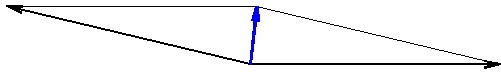
\includegraphics[height=0.055\textwidth]{nn0000.png}
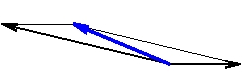
\includegraphics[height=0.055\textwidth]{nn0025.png}

\includegraphics[height=0.055\textwidth]{nn0040.png}

\includegraphics[height=0.055\textwidth]{nn0070.png}

\includegraphics[height=0.055\textwidth]{nn0080.png}

\includegraphics[height=0.055\textwidth]{nn0100.png}
\end{center}
\caption{Initial transient growth followed by ultimate decay resulting
  from the sum (blue) of two non-orthogonal eigenvectors (black), each
  of which decays monotonically.  Adapted from figure~4.1,
  \cite{schmid01}. The asymptotic state is decay dominated by the
  least stable eigenvector. }
\label{fig.tg}
\end{figure}

Now consider energy growth $G$, \ie the ratio of kinetic energies in a
linear disturbance at time $t=\tau$ to that in the initial condition
at time $t=0$.
\begin{equation}
G(\tau)=\frac{E(\tau)}{E(0)}=
\frac{(\bm{u}'_\tau,\bm{u}'_\tau)}{(\bm{u}'_0,\bm{u}'_0)}=
\frac{(\Mop(\tau)\bm{u}'_0,\Mop(\tau)\bm{u}'_0)}{(\bm{u}'_0,\bm{u}'_0)},
\end{equation}
where the last equality exploits \eqref{eq.STO}.  Our goal is to find
the `most dangerous', or optimal, initial disturbance $\uvec'_0$; the
one that generates the greatest amount of growth $G$ for time interval
$\tau$.  Various routes exist for the computation of such an optimum
\citep{bms12,mbs13}; here we will examine the `eigenvalue approach'.
For now let us state without proof that an adjoint operator,
$\Madj(\tau)$ exists for $\Mop(\tau)$.  This adjoint operator has the
property of commuting with the inner product \eqref{eq.inner} such
that
\begin{equation}
(\Mop(\tau)\uvec,\uvec)=(\uvec,\Madj(\tau)\uvec),
\label{eq.commute1}
\end{equation}
which makes
\begin{equation}
G(\tau) = \frac{(\bm{u}'_0,\Madj(\tau)\Mop(\tau)\bm{u}'_0)}
{(\bm{u}'_0,\bm{u}'_0)},
\end{equation}
where the joint operator $\Madj(\tau)\Mop(\tau)$ is symmetric.  By
re-arrangement we find the eigensystem
\begin{equation}
\Madj(\tau)\Mop(\tau)\bm{u}'_0 = G(\tau)\uvec'_0,
\label{eq.growevp}
\end{equation}
which implies that the optimal growth $G(\tau)$ is the largest
eigenvalue of $\Madj(\tau)\Mop(\tau)$ and $\uvec'_0$, the
corresponding eigenvector, is the optimal (or 'most dangerous')
initial disturbance.  We note that the eigenvectors of the symmetric
joint operator $\Madj(\tau)\Mop(\tau)$ are (when normalised such that
$(\upert_0,\upert_0)=1$) precisely the same as the right singular
vectors of the state transition operator $\Mop(\tau)$, and the growth
$G$ is the square of the corresponding singular value.  The terminal
outcome, $\upert_\tau$, is the corresponding left singular vector
\citep[see \S\,1.2,][]{bbs08b}.  We note that we can either compute
$\upert_\tau$ by evolving $\upert_0$ with the \LNS\ equations over
interval $\tau$, or by finding the corresponding eigenmode of the
transposed joint operator $\Mop(\tau)\Madj(\tau)$.

%=============================================================================
\subsection{The adjoint \NavSto\ equations}
\label{sec.adjoint}

In the previous section we introduced the adjoint state transition
operator for the \NavSto\ equations, $\Madj$.  To go into a full
exposition on adjoints would take us very far afield; the interested
reader is advised to consult \citet{lubo14}, but the brief outline in
\citet{bbs08b} is more in line with our present discussion.  The basic
idea is to use integration by parts in order to find an operator which
commutes with the original under an inner product.  Typically in text
books the inner product is purely spatial, \eg \eqref{eq.inner}, but
in our case the integrals concerned must be over both space and time.
If we define
\begin{equation}
\langle\bm{a},\bm{b}\rangle=\int_0^\tau\int_\Omega \bm{a}(t)\bm{\cdot
  b}(t)\,\cd V\cd t,
\label{eq.inner2}
\end{equation}
then the adjoint velocity variable $\uadj$ commutes with the
\LNS\ operator so that
\begin{equation}
\langle\uadj,\partial_t\upert-L\upert\rangle =
\langle\upert,\partial_t\uadj+L^*\uadj\rangle
\label{eq.commute2}
\end{equation}
in which $\partial_t\uadj+L^*\uadj=0$ represents the adjoint
\NavSto\ equations.  Note that we have skipped over some details here:
first, that the construction of the operator just requires the
commutation holds with compact support (so that boundary conditions
need not be considered initially, whereas more properly they do) and
second that a full treatment requires consideration of the pressure
and incompressibility.  Refer to \citet{bbs08b} and \citet{mbs13} for
more explanation.  For now we quote the result that the incompressible
adjoint \NavSto\ equations may be written (semi-symbolically)
\begin{equation}
\partial_t\uadj =
-\left[\bm{I}-\bm{\nabla}\nabla^{-2}\bm{\nabla\cdot}\right]
\left[-\Ubase\bm{\cdot\nabla}
  +\bm{\nabla\Ubase}\bm{\cdot}\right]\uadj
- \Rey^{-1}\nabla^2\uadj.
\end{equation}

Owing to the negative sign on the viscous diffusion operator in the
above, these equations must be integrated backward in time.  This
means that timestepping the equations evolves a terminal condition
$\uadj(\tau)$ backwards in time, as suggested in
figure~\ref{fig.backwards}.  Analogously to the forwards-in-time state
transition operator $\Mop$ we now have the backwards-in-time adjoint
operator $\Madj$ where
\begin{equation}
\uadj(0) = \Madj(\tau)\uadj(\tau).
\end{equation}
In order to apply the joint operator $\Madj(\tau)\Mop(\tau)$ we have
to first evolve the initial condition $\upert_0$ forwards over
interval $\tau$ with $\Mop$ to arrive at $\upert_\tau$, then use the
adjoint operator $\Madj$ to evolve the outcome backwards to $t=0$, as
sketched in figure~\ref{fig.toandfro}.  This amounts to the
left-hand-side of \eqref{eq.growevp}.

\begin{figure}
\begin{center}
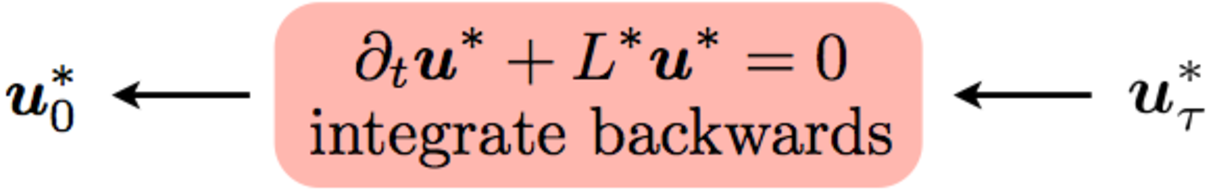
\includegraphics[width=0.4\textwidth]{backwards}
\end{center}
\caption{Applying the adjoint operator $\Madj(\tau)$ to evolve a final
  condition backwards in time.}
\label{fig.backwards}
\end{figure}

\begin{figure}
\begin{center}
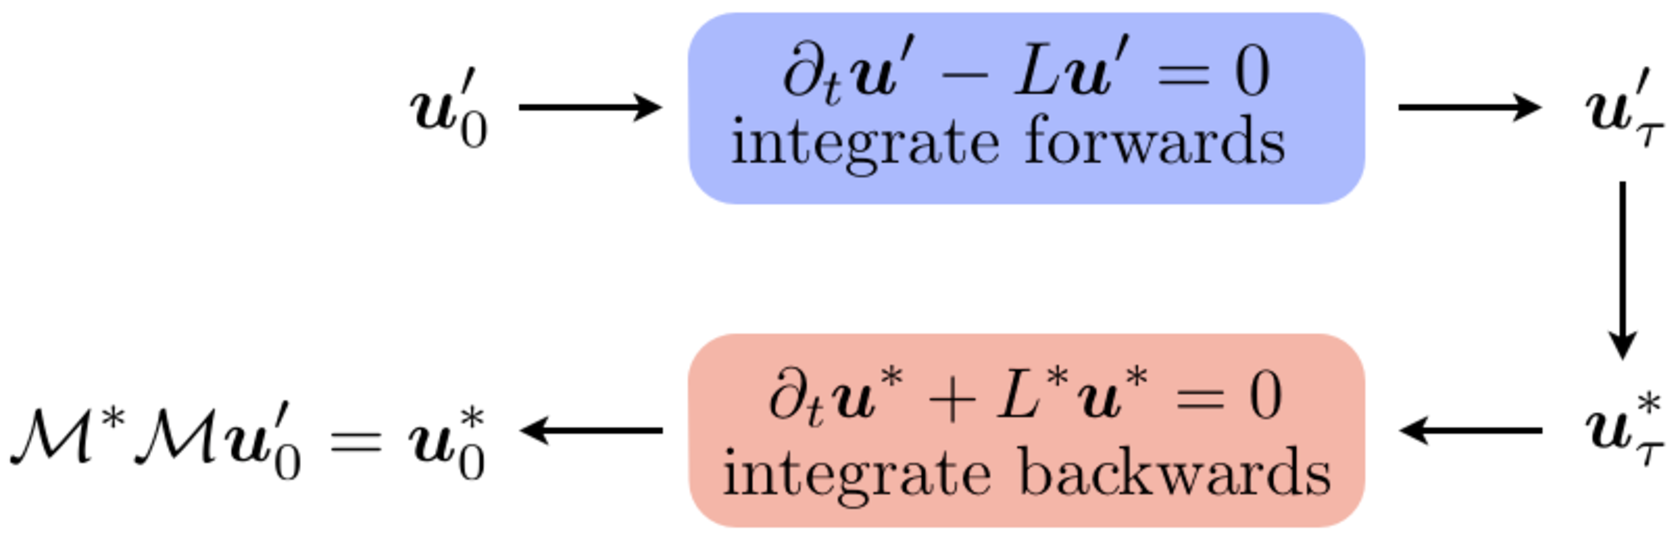
\includegraphics[width=0.525\textwidth]{forwardsbackwards}
\end{center}
\caption{Applying the joint operator $\Mop(\tau)\Madj(\tau)$ to evolve
  an initial condition.}
\label{fig.toandfro}
\end{figure}

Finally we note that more consideration is merited of the argument by
which commutation under the space-time inner product
\eqref{eq.commute2} also allows that in the purely spatial one of
\eqref{eq.commute1}, and that eigensystem approaches are not the only
alternative for computing optimal initial conditions using
timestepping; optimisation-based approaches are also common. Please
consult \citet{schmid07}, \cite{bbs08b} and \citet{mbs13}.

%-----------------------------------------------------------------------------
\subsection{Boundary conditions for transient analysis}
\label{sec.tgbcs}

In simplifying the commutation \eqref{eq.commute2}, which involves
integration by parts, we assume that the perturbation velocity field
(and its adjoint) are zero on all boundaries, and we will need to set
this requirement via wall-type boundary condition specifications on
all domain boundaries in our session files (see
\S\,\ref{sec.bfstg}). This is also convenient as we can use the same
boundary condition set for both the forwards and backwards
integrations. However, for our analysis to be accurate in open flows,
we need to ensure that the domain is of large enough extent both
upstream and downstream in order to contain the perturbation field in
both forwards and backwards integrations.  In practice this means
checking that the optimal initial and terminal conditions $\upert_0$
and $\upert_\tau$ are well contained inside the domain for all values
of $\tau$. See \S\,2.1 of \citet{bbs08a}.

%-----------------------------------------------------------------------------
\subsection{Base flows for transient analysis}
\label{sec.tgbase}

For a transient analysis the base flow's temporal behaviour is not
restricted: it may be steady, periodic, or take any form provided it
can be adequately represented/reconstructed in the solver. If the base
flow is not steady then we also logically need to consider the
temporal phase relative to the base flow at which the disturbance is
initiated \citep[see e.g.][]{bsb08}.

%-----------------------------------------------------------------------------
\subsection{Global optima, temporal evolution of disturbance energy}
\label{sec.envelope}

A point to note is that the time horizon $\tau$ is a parameter in a
transient growth study.  For each $\tau$, there is a local optimum
initial perturbation which gives rise to energy growth $G(\tau)$.  If
the base flow is asymptotically stable there will be a particular time
horizon $\tau_\textrm{opt}$ which produces the global optimal growth
$G_\textrm{max}$. For any $\tau$, evolution of each local optimal
initial disturbance produces a trajectory of flow kinetic energy
which, when normalised by the initial energy, osculates the envelope
$G(\tau)$ at time $\tau$ and lies below it at other times.  These
concepts are illustrated in figure~\ref{fig.eve}. Naturally, attention
is typically focused on the global optimum $G_\textrm{max}$.

\begin{figure}
\begin{center}
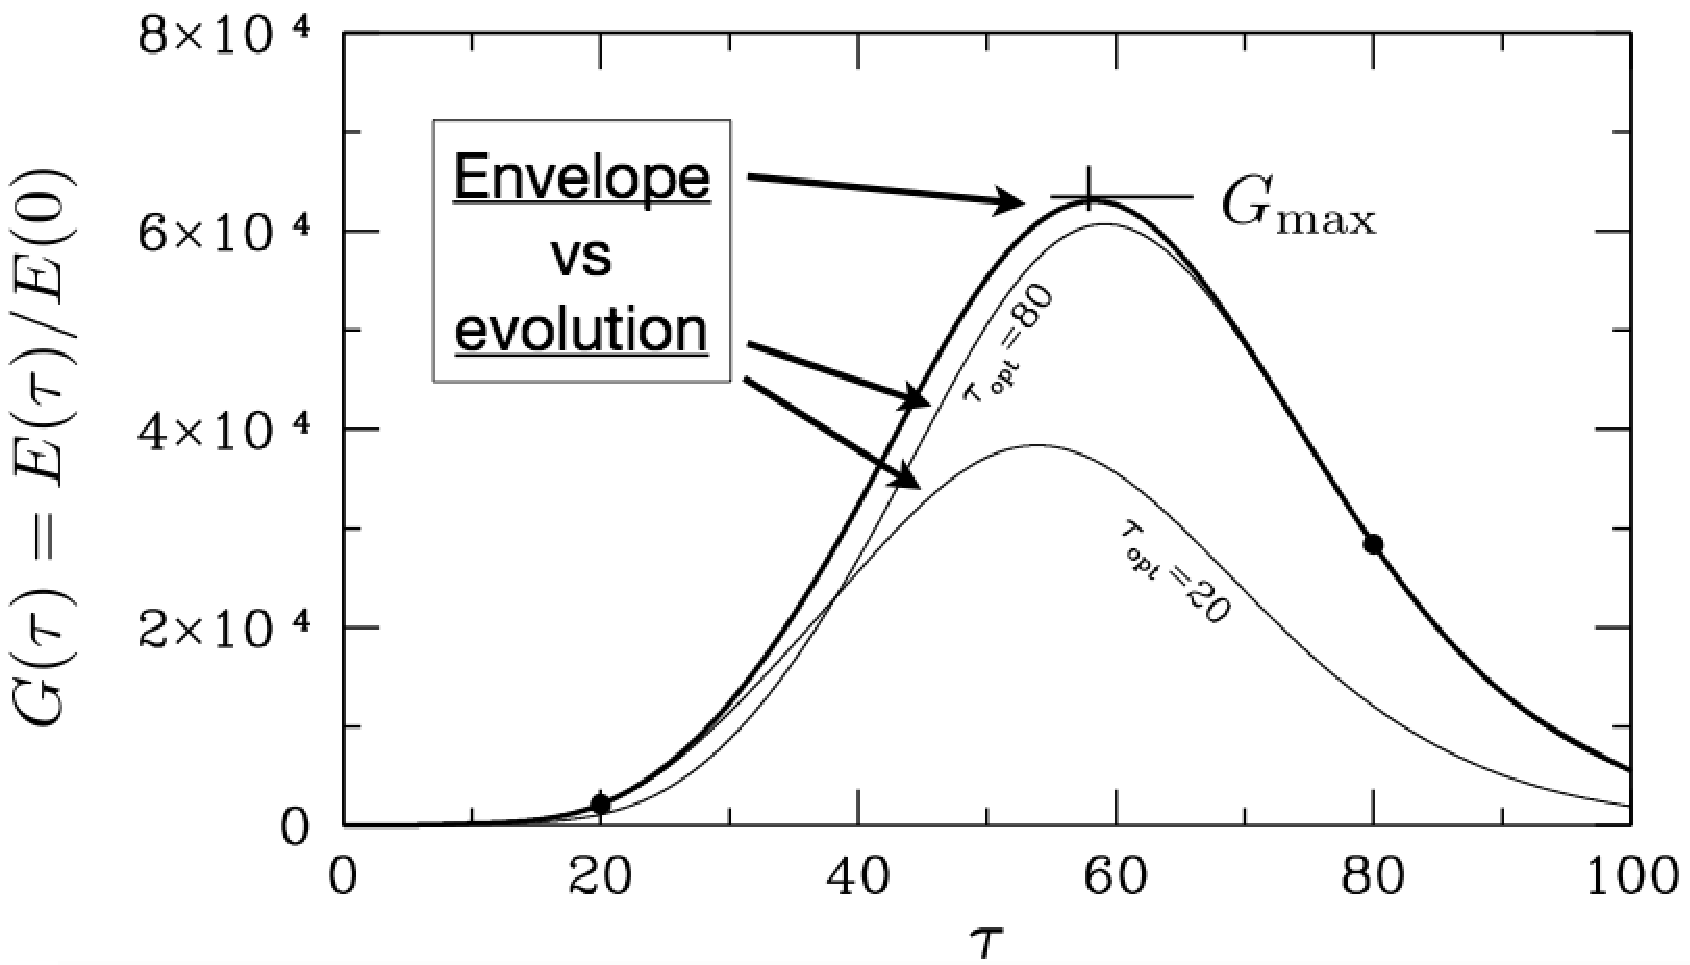
\includegraphics[width=0.55\textwidth]{EnvelopeVsEvolution}
\end{center}
\caption{The concept of global optimal initial disturbance.}
\label{fig.eve}
\end{figure}

At large times, evolution of energy is typically dominated by the
least stable eigenpair of the system, either decaying or growing
expoenntially in time depending on whether the flow is stable or
unstable.

%=============================================================================
\section{Eigensystem solution methods}
\label{sec.outer}

Our timestepper approach to computing eigenmodes for asymptotic
stability or optimal disturbances for finite-time energy growth in the
\LNS\ system in both cases depend on iterative Krylov-based methods
which rely on being able to apply an operator repeatedly to an initial
condition. (The simplest algorithm of this kind is the standard `power
method' for finding eigenvalues and eigenvectors.)  The great
advantage of these techniques is that we do not explicitly need to
construct a matrix which represents the operator\,---\,rather
difficult in the case of unsteady base flows\,---\,instead, we just
have to be able to apply it repeatedly to an initial condition.  So we
can use a common 'outer loop' iterative eigensystem solver, with the
'inner loop' replaced by one of $\Mop(\tau)$, $\Madj(\tau)$,
$\Madj(\tau)\Mop(\tau)$ or $\Mop(\tau)\Madj(\tau)$ depending on the
problem of interest.\footnote{Respectively these inner loop operators
  are applied by issuing the following calls to \Dog:
  $\Mop(\tau)\Longleftrightarrow\texttt{dog}$ (default mode of
  operation); $\Madj(\tau)\Longleftrightarrow\texttt{dog~-a}$;
  $\Madj(\tau)\Mop(\tau)\Longleftrightarrow\texttt{dog~-g}$;
  $\Mop(\tau)\Madj(\tau)\Longleftrightarrow\texttt{dog~-s}$.}

A diagram of the simple Arnoldi-type method described in
\citet{bbs08b} is presented in figure~\ref{fig.DBA}; this represents
the default outer-level operation of \verb+dog+.  Alternatively, one
may use the implicitly restarted Arnoldi method supplied in
\verb+ARPACK+ \citep{lehoucq98} by compiling and running \verb+dog-AR+.

\begin{figure}
\begin{center}
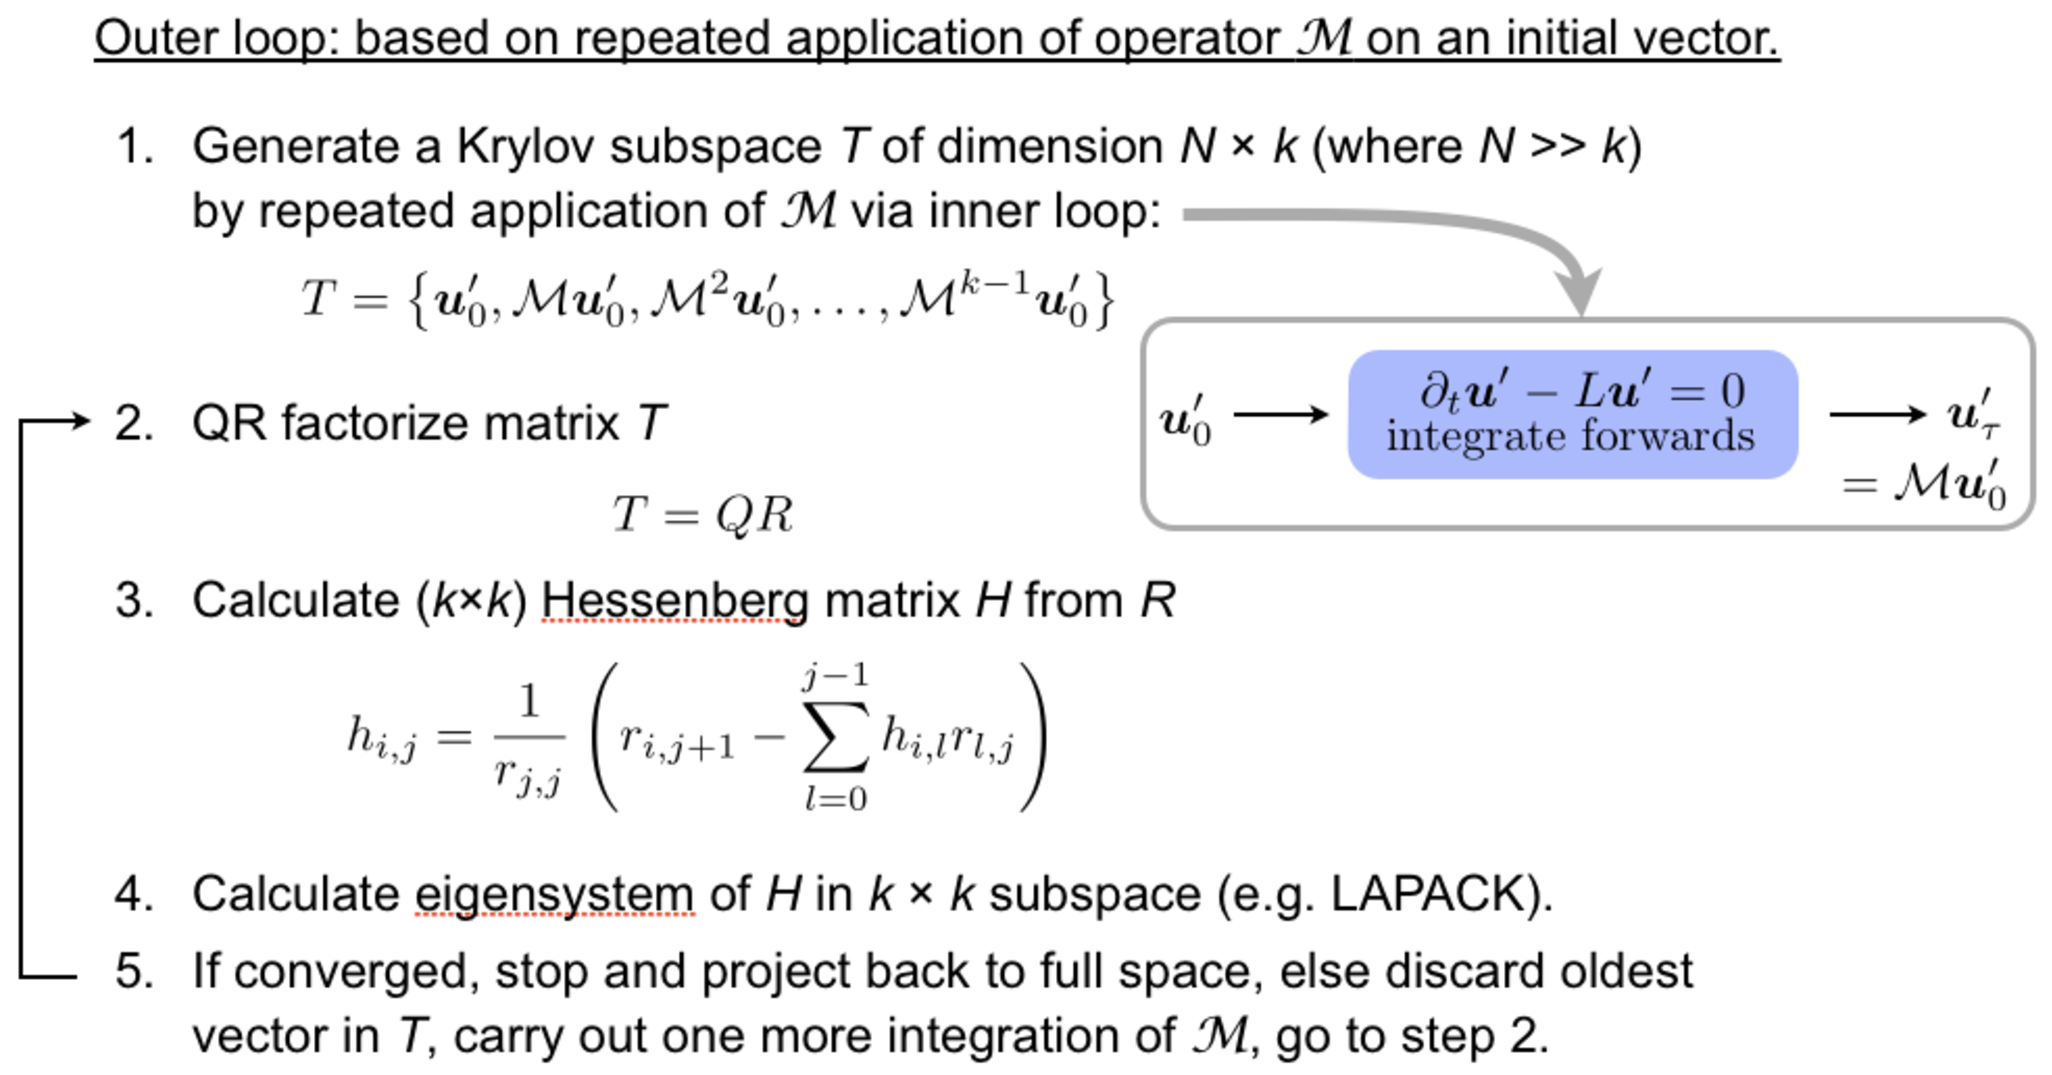
\includegraphics[width=0.9\textwidth]{DBAlgorithm}
\end{center}
\caption{Outer-level iteration for solving an eigenvalue problem via
  timestepping. See \S\,3.2 of \citet{bbs08b} for more detail.}
\label{fig.DBA}
\end{figure}

%=============================================================================
\section{Pros and cons of time-stepper methods for eigensystems}
\label{sec.procon}

Timestepper based methods are not the only answer for these
eigensystem type problems. The other main option would be to first
explicitly construct a matrix representing the operator in question
and then find its eigensystem, something which is not always easy, or
affordable.  Please see \citet{tuba00} for more background and other
applications.

%-----------------------------------------------------------------------------
\subsection{Strengths}
\begin{conlista}
\item
Naturally converges eigenvalues with largest real parts (the `most
dangerous' ones) first.
\item
Easy to develop codes starting from unsteady \NavSto\ solvers.
\item
Not memory intensive.
\item
Works even when it is not conceptually simple to create a matrix
representing the operator in question (\eg Floquet problems).
\end{conlista}

%-----------------------------------------------------------------------------
\subsection{Weaknesses}
\begin{conlista}
\item
Typically can only solve for a comparatively limited number of modes.
\item
For optimal growth, each time horizon $\tau$ requires a new solution
from scratch.
\item
Not simple to apply when shifting is required.  See \citet{gpbt15}
for further discussion.
\item
No way to extract the operator $L$ if it is required for other analyses.
\end{conlista}

%%%%%%%%%%%%%%%%%%%%%%%%%%%%%%%%%%%%%%%%%%%%%%%%%%%%%%%%%%%%%%%%%%%%%%%%%%%%%%
\chapter{Stability analysis of steady flows}
\label{ch.stab}

It is assumed that you already have some familiarity with \Semtex.
The DNS tool from \Semtex, \texttt{dns}, is typically (though as you
will find out in the first example, not always) used to generate the
base flows on which analysis is performed.


%=============================================================================
\section{Two-dimensional stability of Poiseuille channel flow
\protect\footnote{Input files for this example are supplied in
\texttt{dog/testcases/Steady/channel}.}
}
\label{sec.chan2d}

The \twod\ parabolic-profile flow in a parallel channel becomes
linearly unstable to Tollmein--Schlichting waves at $\Rey=5772$
\citep{ors71}.  This is a 1D2C base flow that has 2D2C instability
modes. For $\Rey=7500$ and at streamwise wavenumber $\alpha=1$ (\ie a
wavelength of $2\pi$) based on the centreline velocity and
semi-channel width, \citet[\S\,1.4]{chqz88} supply estimates of the
eigenvalue $\lambda=0.00223497+\ci 0.24989154$ (the temporal growth
rate is the first of these values and the second is the temporal
circular frequency).  This is a rather simple problem because the
domain is rectangular, the base flow is analytic, and also the
eigenmode is 2D2C\,---\,\twod\ and \twoc.  (While a global stability
analysis is overkill for this problem, it certainly is
straightforward.)

First, we'll make a session file. Since the domain is rectangular, we
can use the \Semtex\ \verb+rectmesh+ utility, which makes a start-up
session file that we can edit to create a workable session file for
our problem.  Below is the rectmesh input file (made with a text
editor) that we'll call \verb+channel.rect+.  The format is: list of
$x$-locations; blank line; list of $y$-locations.  Don't worry that
the length is initially $\Delta x=2$ rather than $2\pi$; we will fix
that by editing the session file that we produce.

{\small
\begin{verbatim}
-1
-0.75
-0.5
-0.25
0
0.25
0.5
0.75
1

-1
-0.8
-0.5
0
0.5
0.8
1
\end{verbatim}
}

Next we create our session file:
{\small
\begin{verbatim}
[mec-aquila]$ rectmesh channel.rect > channel
\end{verbatim}
}

Edit the resulting session file to produce:
{\small
\begin{verbatim}
<TOKENS>
        X_SCALE  = PI

        N_SLICE  = 1
        N_BASE   = 2

        N_TIME   = 2
        N_P      = 11
        N_STEP   = 200
        D_T      = 0.005
        Re_D     = 7500
        KINVIS   = 1/Re_D

        IO_HIS   = 20
        IO_FLD   = 1000
        IO_CFL   = 20
</TOKENS>

<FIELDS NUMBER=3>
        u      v       p
</FIELDS>

<GROUPS NUMBER=1>
        1       w       wall
</GROUPS>

<BCS NUMBER=1>
        1       w       3
                <D>     u = 0.0  </D>
                <D>     v = 0.0  </D>
                <H>     p        </H>
</BCS>

<USER>
        u = 1-y*y
        v = 0.
        p = 0.
</USER>

<NODES NUMBER=63>
    1	             -1             -1              0
    2	          -0.75             -1              0
    ..
    ..
    62	           0.75              1              0
    63	              1              1              0
</NODES>

<ELEMENTS NUMBER=48>
    1	<Q>    1    2   11   10    </Q>
    2	<Q>    2    3   12   11    </Q>
    ..
    ..
    47	<Q>   52   53   62   61    </Q>
    48	<Q>   53   54   63   62    </Q>
</ELEMENTS>

<SURFACES NUMBER=22>
         1   1  1  <B>  w  </B>
        ..
        ..
         8   8  1  <B>  w  </B>

         9  41  3  <B>  w  </B>
        ..
        ..
        16  48  3  <B>  w  </B>

        17   8  2  <P>   1  4  </P>
        ..
        ..
        22  48  2  <P>  41  4  </P>
</SURFACES>
\end{verbatim}
}
\noindent
(Note that various repetitious lines have been deleted from the above
listing.)  The spectral element mesh (as obtained from the session
file using the \verb+meshpr+ utility) is shown in
figure~\ref{fig.chanmesh}.

\begin{figure}
\begin{center}
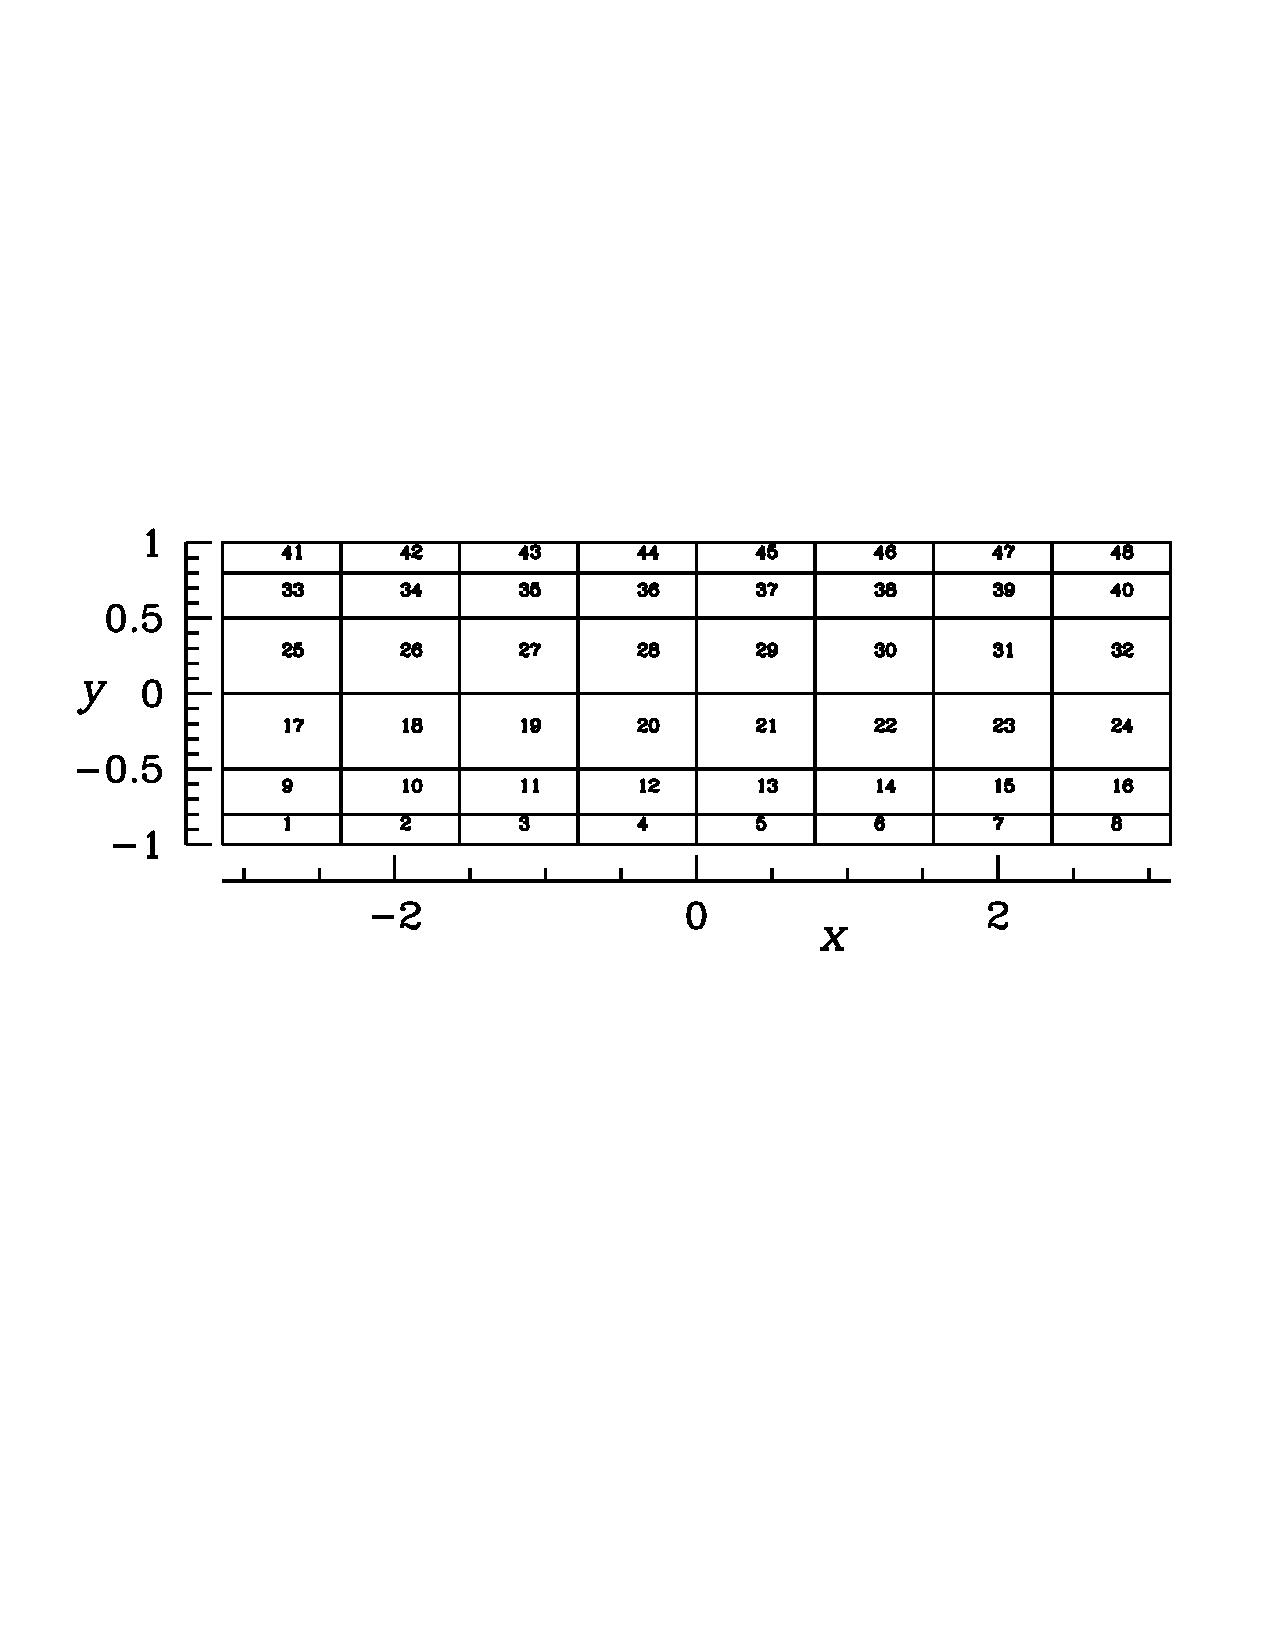
\includegraphics[width=0.6\textwidth]{channel_mesh}
\end{center}
\caption{Spectral element mesh (with element numbers) for Poiseuille
  flow in a channel.}
\label{fig.chanmesh}
\end{figure}

%-----------------------------------------------------------------------------
\subsection{\texttt{TOKENS} section}

Let us first examine the \verb+TOKENS+ used.  Setting
\verb+X_SCALE=PI+ is used to expand the overall length of the domain
to $2\pi$ (this scaling is not specific to \Dog, but is a normal part
of \Semtex).  
%
The next two tokens are, however, specific to \Dog: \verb+N_SLICE=1+
says that there will be only a single time-slice in the base flow file
(the base flow is steady in time), while \verb+N_BASE=2+ stipulates
that the base flow should only have two velocity components ($x$ and
$y$ components $u$ and $v$).
%
Setting \verb+N_TIME=2+ stipulates 2nd-order accurate time stepping
(this could be omitted since it is the default value, but you may
occasionally want to use \verb+N_TIME=1+ or
\verb+N_TIME=3+). \verb+N_P=11+ will give 11 mesh points along the
side of each quadrilateral element so that the element shape functions
will be tensor products of 10th-order GLL-Lagrange interpolants.
%
\verb+N_STEP=200+ and \verb+D_T=0.005+ together mean that the
time-step is $\Delta t=0.005$ and 200 steps are taken for each
integration of the linearised \NavSto\ equations over an interval
$\tau=1$ between Arnoldi updates.  Both these values (time step
and interval between updates) ultimately need to be chosen on the
basis of trial and error\,---\,at least, that is the case for a steady
flow stability analysis: for a time-periodic base flow the interval is
pre-determined and only the time-step needs to be set.
%
\verb+Re_D=7500+ and \verb+KINVIS=1/Re_D+ are used to set the
kinematic viscosity: we could have directly set
\verb+KINVIS=0.0001333333333+ but here we see the built-in function
parser used to set the value (token \verb+Re_D+ is not otherwise
significant to the solver).

%-----------------------------------------------------------------------------
\subsection{\texttt{FIELDS} section}

This is used to tell the solver that 3 fields will be be used and they
are two velocity components $u$ and $v$ along with pressure $p$.  NB:
the pressure is not normally considered to be part of the eigensystem
and further that the pressure variable contained in the
\verb+session.eigX+ file is normally unreliable (BUT one can force it
to be included using the \verb+-p+ command-line option to
\verb+dog+). Also note that the \verb+NUMBER+ of fields must be
specified in the section header (this is not required in normal
\Semtex\ usage).

%-----------------------------------------------------------------------------
\subsection{\texttt{GROUPS} and \texttt{BCS} sections}

Standard \Semtex\ usage. Read that user guide!

%-----------------------------------------------------------------------------
\subsection{\texttt{USER} section}

While again this is standard \Semtex\ usage, we note that in the
present case we will be using this section along with the standard
utility \texttt{compare} in order to generate our base flow.  Again
observe the implied use of the built-in function parser to deal with
the string \verb+u = 1-y*y+ and that coordinate \verb+y+ (along with
\verb+x+ and \verb+t+) is known to the parser.

%-----------------------------------------------------------------------------
\subsection{\texttt{NODES}, \texttt{ELEMENTS} and \texttt{SURFACES} sections}

Standard \Semtex.  However, note the use of \verb+<P>+ in the
\verb+SURFACES+ section to declare periodic edges.  This is typically
appropriate for problems which have a homogeneous direction (and which
could just as well be tackled by a non-global approach).

%-----------------------------------------------------------------------------
\subsection{Base flow generation}

Normally we would have to use \texttt{dns} to generate a steady base
flow (typically by integrating to reach the asymptotically steady
state, a task which might well require its own session file and time
stepping).  In the present case, though, have an analytic base flow
declared in our session file and can use the \verb+compare+ utility to
parse the strings in the \verb+USER+ section.
{\small
\begin{verbatim}
[mec-aquila]$ compare channel > channel.bse
\end{verbatim}
} This creates a base flow with $u=1-y^2$, $v=0$ and $p=0$ (the
pressure is not used and could in fact be omitted).

%-----------------------------------------------------------------------------
\subsection{Make an enumeration file}

We have retained the standard \Semtex\ requirement that a
\verb+session.num+ file must be produced. If not explicitly created,
one will be generated on the fly, but it is usually better to make one
`by hand' in order to ensure that the highest-level RCM numbering
optimisation level (3) is obtained.  {\small
\begin{verbatim}
[mec-aquila]$ enumerate -O3 channel > channel.num
\end{verbatim}
}

%-----------------------------------------------------------------------------
\subsection{Running \texttt{dog}}

Now we are ready. I'll assume commands from \Dog\ (like all the
\Semtex\ commands we've used to this point) will be found in your
\texttt{PATH}.
{\small
\begin{verbatim}
[mec-aquila]$ dog -k 16 -n 1 -m 500 -t 1e-6 channel > /dev/null &
\end{verbatim}
}The command line arguments above have the following significance:
\verb+-k 16+; set the Krylov dimension to 16, \verb+-n 1+; stop after
one eigenvalue is converged to the requested tolerance,
\verb+-m 500+; iterate for a maximum of 500 iterations, \verb+-t 1e-6+;
carry on converging until the residual for the highest-numbered
eigenvalue requested (here just one) falls below this tolerance value
(\textbf{multiplied by the growth magnitude}).

The first time you run \verb+dog+ you might not want to suppress the
standard output as we have done here in order to ensure everything is
running correctly. However, the usage above is generally standard
since it allows the user to monitor convergence of the eigensystem
solver by running \verb+tail+ on the \verb+session.evl+ file.  {\small
\begin{verbatim}
[mec-aquila]$ tail -f channel.evl
\end{verbatim}
} This will show us updates to the end of the eigenvalue file.  After
a number of iterations the solution terminates with {\small
\begin{verbatim}
-- Iteration = 265, H(k+1, k) = 0.894358
EV  Magnitude   Angle       Growth      Frequency   Residual
 0  1.0022e+00  2.4989e-01  2.2358e-03  2.4989e-01  9.7943e-07
 1  1.0022e+00 -2.4989e-01  2.2358e-03 -2.4989e-01  9.7943e-07
 2  9.6002e-01  9.5902e-01 -4.0801e-02  9.5902e-01  1.6653e-03
 3  9.6002e-01 -9.5902e-01 -4.0801e-02 -9.5902e-01  1.6653e-03
 4  9.9859e-01  0.0000e+00 -1.4078e-03  0.0000e+00  5.2856e-03
 5  9.9644e-01  0.0000e+00 -3.5696e-03  0.0000e+00  1.4456e-02
 6  9.4387e-01  1.9403e+00 -5.7764e-02  1.9403e+00  3.7580e-02
 7  9.4387e-01 -1.9403e+00 -5.7764e-02 -1.9403e+00  3.7580e-02
 8  9.8493e-01  0.0000e+00 -1.5188e-02  0.0000e+00  4.1501e-02
 9  9.2051e-01  2.9086e+00 -8.2826e-02  2.9086e+00  2.3085e-01
10  9.2051e-01 -2.9086e+00 -8.2826e-02 -2.9086e+00  2.3085e-01
11  8.9517e-01  1.6337e+00 -1.1075e-01  1.6337e+00  3.5807e-01
12  8.9517e-01 -1.6337e+00 -1.1075e-01 -1.6337e+00  3.5807e-01
13  7.6534e-01  2.2901e+00 -2.6743e-01  2.2901e+00  7.4006e-01
14  7.6534e-01 -2.2901e+00 -2.6743e-01 -2.2901e+00  7.4006e-01
15  2.8354e-01  3.1416e+00 -1.2604e+00  3.1416e+00  8.3424e-01
dog: converged, writing 1 eigenvectors.
\end{verbatim}
} 

%-----------------------------------------------------------------------------
\subsection{Examining the outputs}

You should find that file \verb+channel.eig.0+ now exists: this is the
leading eigenvector (not written out unless convergence is obtained):
we only get one because only one was requested (\verb+-n 1+).  In fact
since the leading eigenvalue is complex, we could have converged both
the leading eigenvector and its `complex conjugate' which in this case
will be real-valued, just like the leading eigenvector, but
phase-shifted a quarter-period in time, \ie translated along the
channel. We will return to that point below.

Let us examine the significance of the listing above from
\verb+channel.evl+.  The first point is that 265 iterations were
required for convergence, largely reflecting the fact that there is
not a great deal of separation of the magnitudes of the leading
eigenvalues, as an inspection of the less-converged values indicates.
The \verb+EV+ column refers to the eigenvalue index (starting at 0),
of which there are 16 reported values corresponding to the Krylov
dimension requested on the command line (\verb+-k 16+).  The
\verb+Magnitude+ and \verb+Angle+ columns are for the (estimated)
eigenvalues $\mu_j$ of the state transition operator $\Mop(\tau)$ (see
\ref{eq.map}), while the \verb+Growth+ and \verb+Frequency+ columns
are the real and imaginary parts of the eigenvalues $\lambda_j$ of
$\Lop$ as derived from $\mu_j$ via \eqref{eq.convert}.  We note that
(since $\tau=1$) the \verb+Angle+ and \verb+Frequency+ values are
identical, while the \verb+Growth+ and \verb+Magnitude+ values are
related by $\lambda_{r,j}=\ln(|\mu_j|)/\tau$ (in fact, owing to
rounding, it is better here to confirm that $|\mu_j| =
\exp(\tau\lambda_{r,j})$).  Finally, the \verb+Residual+ column.  The
value reported is the Arnoldi-method residual value $\varepsilon$ as
described on page 1449 of \citet{bbs08b}, but there is a slight change
to the methodology: convergence is deemed to have occurred when
$\varepsilon_j\mu_j<\textrm{tol.}$ for all the eigenvalue estimates
requested, where $\textrm{tol.}$ is the value specified on the command
line via the \verb+-t+ argument (default value
$\textrm{tol.}=1\times10^{-6}$). In the present case that means
convergence would have been obtained on the first eigenvalue estimate
once the residual was below $1.0022\times10^{-6}$.

Now we have explained the significance of these values, we may remark
on the satisfactory agreement between the leading eigenvalue reported
in \citet{chqz88} ($\lambda=0.00223497+\ci 0.24989154$) and what we
computed ($\lambda=0.0022358+\ci 0.24989$). Without some (advisable)
further checking on convergence of our results it is difficult to
conclude which is more accurate, but we can accept that the values are
the same to `plotting' accuracy, at least.

Before going on, let us re-run the previous analysis but ask for the
two leading eigenvectors (\verb+-n 2+).  Nothing much changes, except that
at the end of \verb+channel.evl+ \Dog\ will report `\texttt{writing 2
  eigenvectors}' and now we will have \verb+channel.eig.0+ and
\verb+channel.eig.1+. The $x$- and $y$-component velocities ($u$ and
$v$) of the two eigenmodes are shown in figure~\ref{fig.chanmodes}.
Note their periodicity in the streamwise ($x$) direction.

Generate a \Tecplot\ input file (can also be read by \Paraview)
like this:
\begin{verbatim}
[mec-aquila]$ meshpr channel | sem2tec channel.eig.0
\end{verbatim}
\noindent which should create \verb+channel.eig.0.plt+.

\begin{figure}
\begin{center}
\raisebox{27ex}{(a)}
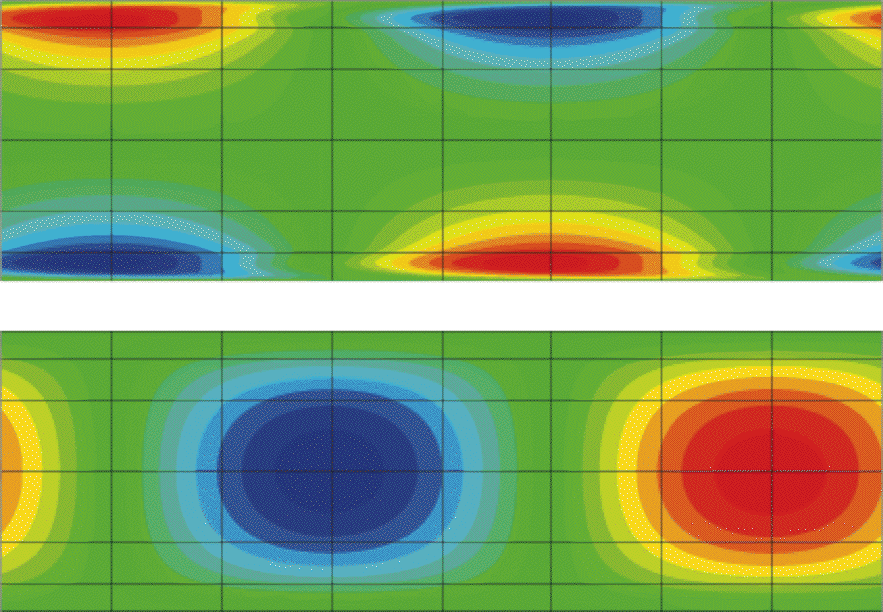
\includegraphics[width=0.45\textwidth]{export0.pdf}
\raisebox{27ex}{(b)}
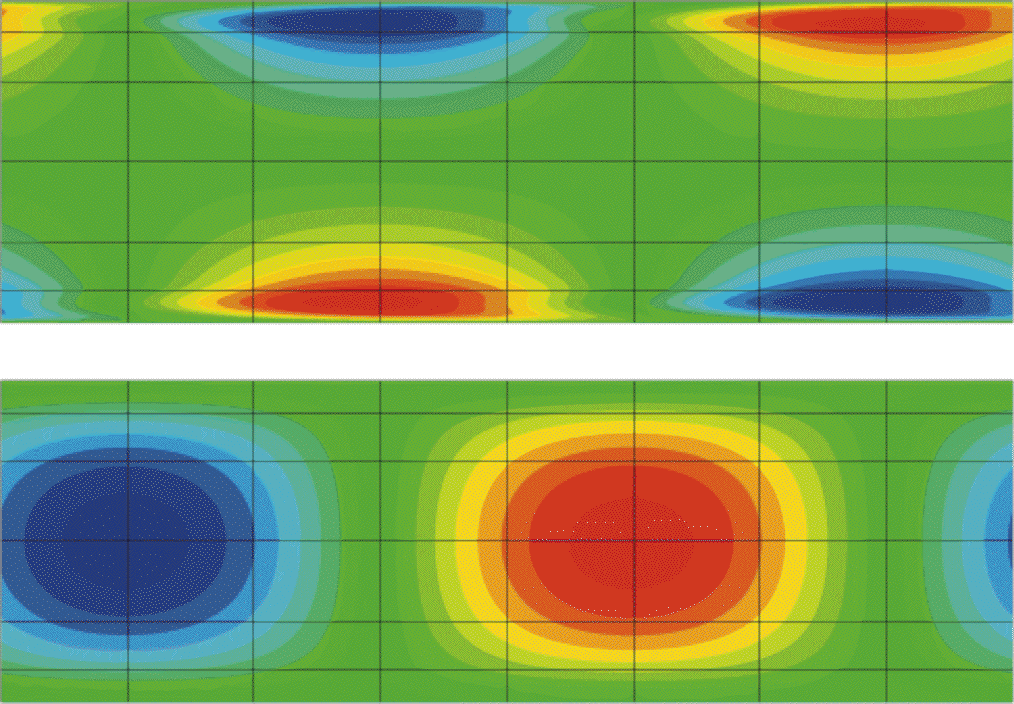
\includegraphics[width=0.45\textwidth]{export1.pdf}
\end{center}
\caption{Contour plots of (upper) $u'$ velocity component and (lower)
  $v'$ velocity component of leading eigenmodes (a) 0 and (b) 1 of
  Poiseuille channel flow, $\Rey=7500$.}
\label{fig.chanmodes}
\end{figure}

The eigenmodes have a wavy structure which is appropriate since they
represent a Tollmein--Schlichting type instability; the mode shapes
are representative of an array of counter-rotating rolls which
propagate streamwise.  It is worth pointing out that, like all
eigenmodes, the choice of sign is arbitrary (the sign affects both
velocity components at once), so one could swap red and blue contours
and still have valid eigenmodes.  Also the scaling of the modes is
arbitrary.  We observe that a definite spatial phase relationship
exists between modes 0 and 1: the anti-nodes of mode~1 interleave those
of mode~0, or equivalently there is a quarter-wavelength phase shift
between them (much like the relationship between sine and cosine
functions).  Since the corresponding eigenvalues were a
complex-conjugate pair, the (real) eigenmodes have to have this
relationship in order to ensure that the propagating wave
corresponding to the mode could be reconstructed with an arbitrary
phase/spatial location.

We can say how fast the waves propagate down the channel.  Since the
wavelength is (the length of the domain) $2\pi$ and the oscillation
period at every point in the flow is $T=2\pi/0.22489=25.1438$, we
conclude that the propagation speed of the waves is 0.22489.  Hence if
we take one of the eigenmodes as an initial condition and evolve it
using the \LNSE\ for $T/2$ we should find it has increased slightly in
magnitude and travelled half the length of the domain.  We could check
this using the \verb+lns+ utility.  First we edit the \verb+TOKENS+ as
follows:
{\small
\begin{verbatim}
<TOKENS>
        ..
        ..
        N_STEP   = 200
        D_T      = 0.005
omega = 0.24989
period = TWOPI/omega
tevolv = 0.5 * period
N_STEP = 2500
D_T    = tevolv/N_STEP
        Re_D     = 7500
        KINVIS   = 1/Re_D
        ..
        ..
</TOKENS>
\end{verbatim}
} \noindent (Note that the final definitions of tokens \verb+N_STEP+
and \verb+D_T+ over-ride earlier ones. We chose \verb+N_STEP+ such
that the value of \verb+D_T+ is quite similar to what we earlier used,
\verb+0.005+.)  Next we link the first eigenmodes to serve as a
restart file {\small
\begin{verbatim}
[mec-aquila]$ ln -s channel.eig.0 channel.rst
\end{verbatim}
}
\noindent
run \verb+lns+:
{\small
\begin{verbatim}
[mec-aquila]$ lns channel > /dev/null
\end{verbatim}
}
\noindent and finally we can examine the output (\verb+channel.fld+)
to verify that it looks much the same as the initial condition, but,
as we expect, translated a length $\pi$ in the $x$ direction (same
shapes, signs inverted). We leave this as `an exercise for the
reader'.

%=============================================================================
\section{Steady \twod\ flow past a circular cylinder
\protect\footnote{Input files for this example are supplied in
  \texttt{dog/testcases/Steady/cylinder}.}  }
\label{sec.cyl2d}

This section deals with the onset of \twod\ vortex shedding in flow
past a circular cylinder.  The base flow is 2D2C, as are the
eigenmodes.  Unlike the channel flow of the last section, this is a
case where a global stability analysis is effectively the only option,
and now we have to compute the base flow prior to stability analysis,
since it is not available as an analytical function.  We will attempt
to estimate the critical Reynolds and Strouhal numbers.  The first
credible numerical study of the problem was by \citet{jack87}; more
recently, \citet{kumi06} detailed blockage dependence of critical
values.  From those studies (and numerous experiments), we expect
$\Rey_c=UD/\nu\approx46$ and $\Str_c=fD/U\approx0.125$ where $U$ is
the background base-flow speed, $D$ is cylinder diameter,
$f=\omega/2\pi$ is frequency, $\nu$ is kinematic viscosity.

Another new consideration is that, very typical of flow stability
analyses, the instability breaks a symmetry of the base flow, which
here is a reflection symmetry in the $x$-axis:
\begin{equation}
(u,v)(x,y)=(u,-v)(x,-y).
\end{equation}
This gives us a problem, because we will be computing the base flow
using time-integration of the unsteady \NavSto\ equations.  Above
$\Rey_c$, the flow is unstable, and so unless we take special action,
the base flows computed on a full domain will become time-periodic.
There are a few ways to circumvent this problem: use a Newton (or
other) method to solve the steady \NavSto\ equations
\citep{tuba00,hmb02a}, use selective frequency damping (SFD) approach
to force a steady state \citep{abhhms06}; or control symmetry by using
appropriate boundary conditions with a semi-domain.  All of these
approaches will work and have been used with \Semtex\ (though Newton
and SFD require non-standard code extensions), but the semi-domain
approach is simplest and arguably fastest.  The spectral element
mesh we will use for this study is shown in
figure~\ref{fig.semicylmesh}; lengths are given in terms of the
cylinder diameter $D$.

\begin{figure}
\begin{center}
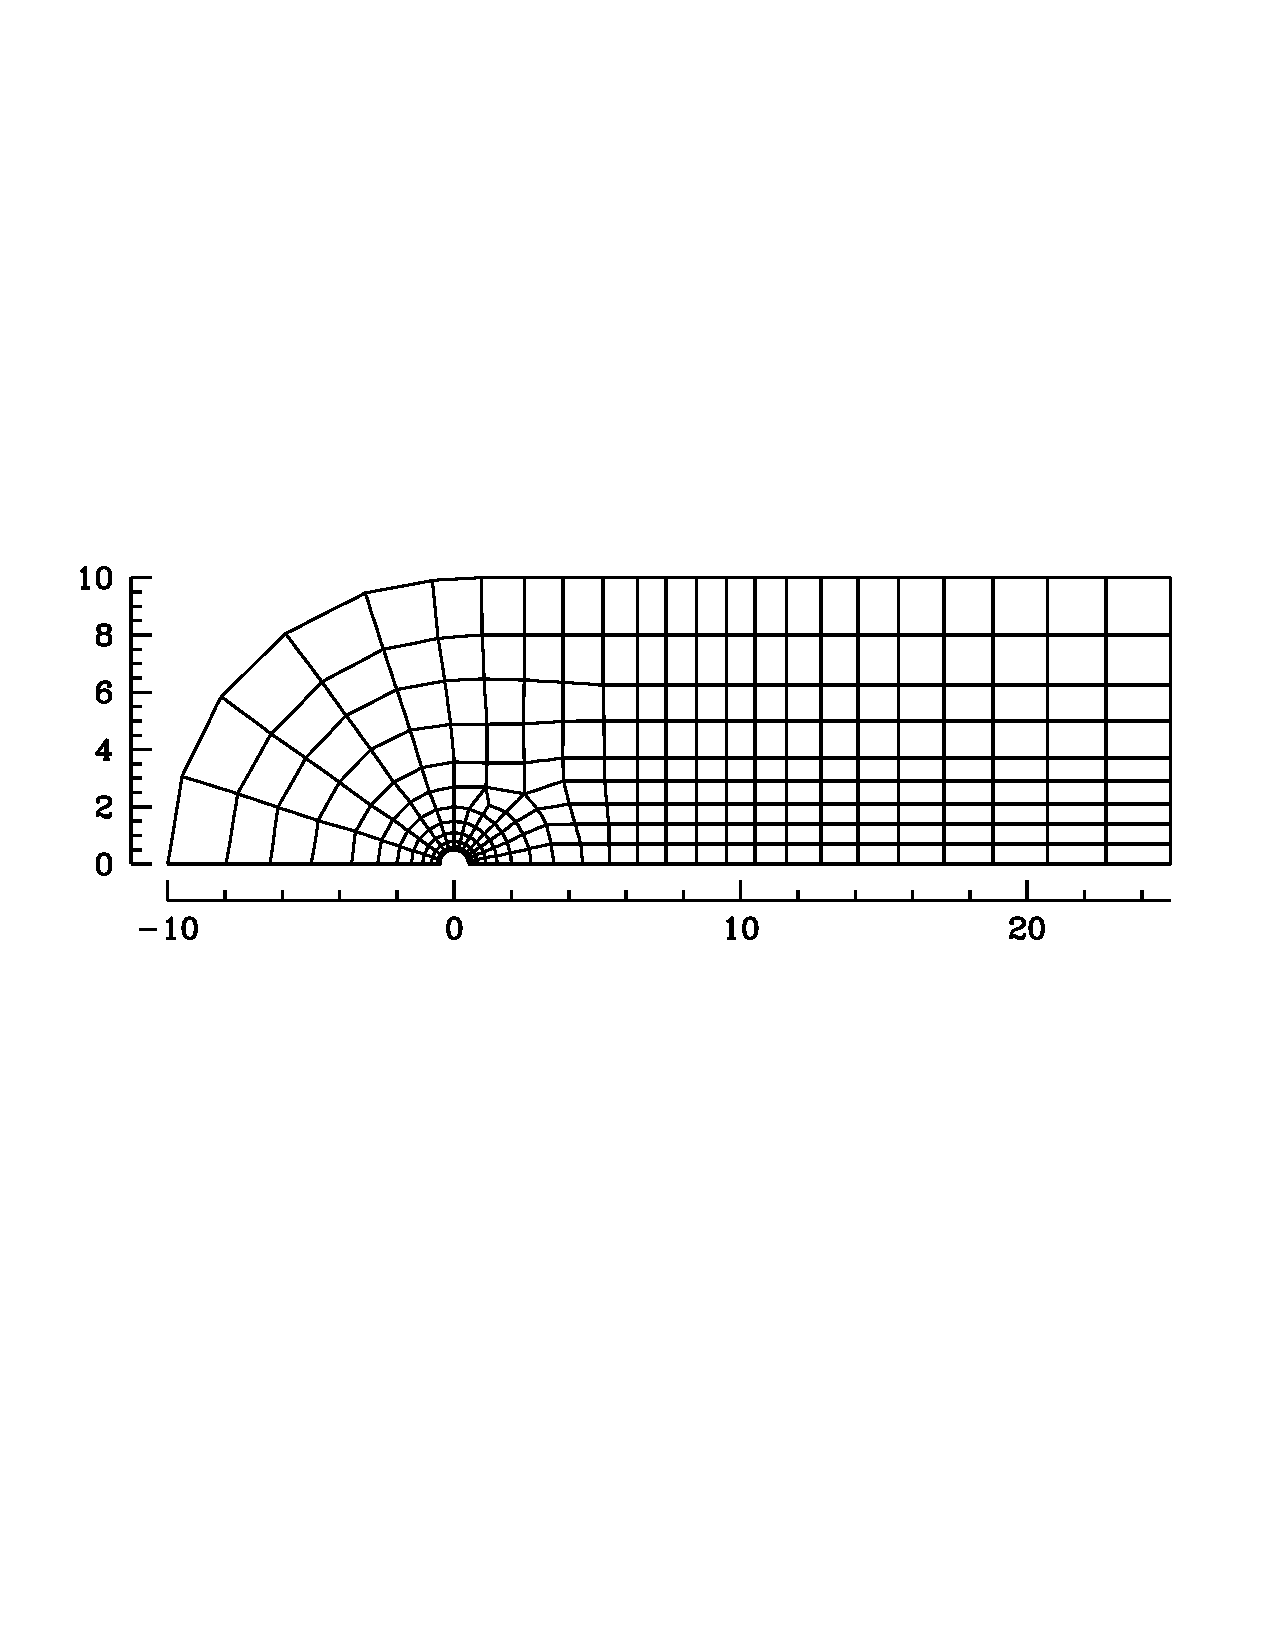
\includegraphics[width=0.65\textwidth]{semicyl02mesh.pdf}
\end{center}
\caption{A semi-domain spectral element mesh for flow past a circular
  cylinder, with 268 elements.}
\label{fig.semicylmesh}
\end{figure}

%=============================================================================
\subsection{Base flow}

A session file for computing the base flow is supplied as
\verb+semicyl02-base+. We will discuss the following sections from
that file: {\small
\begin{verbatim}
<TOKENS>
        Re        = 50.0
        KINVIS    = 1.0/Re
        U         = 1.0
        T_FINAL   = 500
        D_T       = 0.01
        N_STEP    = int(T_FINAL/D_T)
        N_P       = 6
</TOKENS>

<FIELDS NUMBER=3>
        u v p
</FIELDS>

<GROUPS NUMBER=4>
        1       v       velocity
        2       w       wall
        3       o       exit
        4       s       symmetry
</GROUPS>

<BCS NUMBER=4>
        1       v       3
                        <D>     u = U           </D>
                        <D>     v = 0.0         </D>
                        <H>     p               </H>
        2       w       3
                        <D>     u = 0.0         </D>
                        <D>     v = 0.0         </D>
                        <H>     p               </H>
        3       o       3
                        <N>     u = 0.0         </N>
                        <N>     v = 0.0         </N>
                        <D>     p = 0.0         </D>
        3       s       3
                        <N>     u = 0.0         </N>
                        <D>     v = 0.0         </D>
                        <N>     p = 0.0         </N>
</BCS>
\end{verbatim}
} In the \verb+TOKENS+ section we set the kinematic viscosity to give
a Reynolds number of 50 (we plan to bracket the critical Reynolds
number and will carry our analyses at both $\Rey=40$ and $\Rey=50$).
The base flow speed is set as \verb+U=1+; this value will be used to
set the inflow boundary velocity.  We will timestep the base flow for
50 time units from a zero IC (the default) and consider it to be
steady, but in a rigorous study we should be checking that it
\emph{really is} steady (\eg\ by examining history point data). We
have set \verb+N_P=6+; again, this is a reasonable guess but really
demands a resolution check.

The selection of boundary conditions mostly follows standard
\Semtex\ usage; a prescribed far-field velocity $(u,v)=(U,0)$ with a
`high-order' computed Neumann condition on pressure, a zero-slip wall
boundary, an `approximate zero stress' outflow boundary with $\partial
u/\partial n=\partial v/\partial n = p = 0$.  The `symmetry' (or
free-slip/zero-penetration) boundary used on the $x$-axis has
$\partial u/\partial n=v=\partial p/\partial n=0$ to ensure that the
base flows have reflection symmetry $(U,V)(x,y)=(U,-V)(x,-y)$.  Note
that we will later change this boundary condition in the session file
for the stability analysis in order to ensure that the eigenmodes do
break symmetry (and are anti-symmetric).

We run \verb+dns+ to generate the base flow for $\Rey=50$:
\begin{verbatim}
[mec-aquila]$ enumerate -O3 semicyl02-base > semicyl02-base.num; \
 dns semicyl02-base > /dev/null
\end{verbatim}
\noindent
The resulting contours of $U$ are shown in figure~\ref{fig.semibase}.
While we will not go into detail, we also compute the base flow for
$\Rey=40$ (make a copy of the base flow output \verb+.fld+ file, say
to \verb+Re50.bse+, edit \verb+semicyl02-base+ to set \verb+Re=40+;
re-run, copy the new \verb+.fld+ file to \verb+Re40.bse+).  Now we are
in a position to carry out our stability analysis.
\begin{figure}
\begin{center}
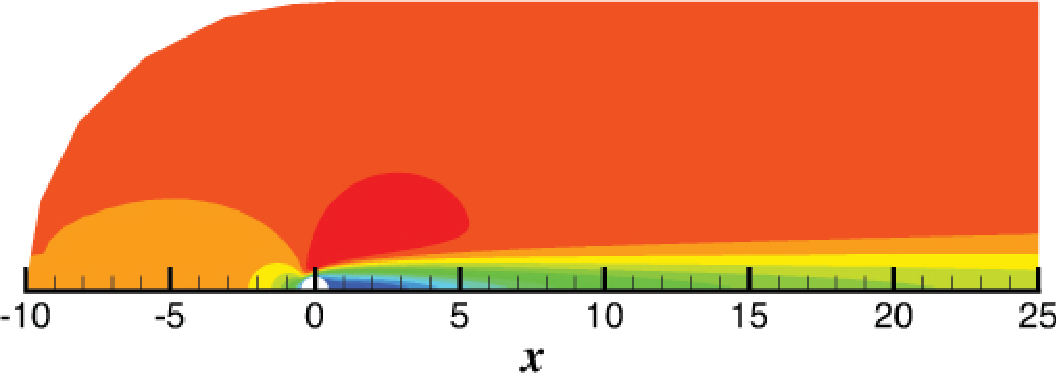
\includegraphics[width=0.65\textwidth]{Re50_base_u.pdf}
\end{center}
\caption{Base flow past a circular cylinder computed on a
  semi-domain. Contours of $U$ at $\Rey=50$.}
\label{fig.semibase}
\end{figure}


%=============================================================================
\subsection{Stability analysis}

First we will look at the section from the stability analysis session
file that differ from the base flow session file. That basically
amounts to adding/changing some \verb+TOKENS+ and altering the BCs.

{\small
\begin{verbatim}
<TOKENS>
        Re        = 50.0
        KINVIS    = 1.0/Re
        U         = 0.0
        N_BASE    = 2
        N_SLICE   = 1
        D_T       = 0.01
        T_FINAL   = 2.0
        N_STEP    = int(T_FINAL/D_T)
        N_P       = 6
</TOKENS>

<FIELDS NUMBER=3>
        u v p
</FIELDS>

<GROUPS NUMBER=4>
        1       v       velocity
        2       w       wall
        3       o       exit
        4       s       symmetry
</GROUPS>

<BCS NUMBER=4>
        1       v       3
                        <D>     u = U           </D>
                        <D>     v = 0.0         </D>
                        <H>     p               </H>
        2       w       3
                        <D>     u = 0.0         </D>
                        <D>     v = 0.0         </D>
                        <H>     p               </H>
        3       o       3
                        <N>     u = 0.0         </N>
                        <N>     v = 0.0         </N>
                        <D>     p = 0.0         </D>
        3       s       3
                        <D>     u = 0.0         </D>
                        <N>     v = 0.0         </N>
                        <D>     p = 0.0         </D>
</BCS>
\end{verbatim}
}
\noindent
In the \verb+TOKENS+ section, note that the Reynolds number (or
\verb+KINVIS+) must be set to match the value used to compute the base
flow\,---\,this seems obvious but it is easy to overlook. Also note
that the far-field velocity is now set (via \verb+U = 0+) to
$(u',v')=(0,0)$, which is appropriate since we expect the domain to
be large enough to contain the perturbation at the far-field
boundaries. Again it is easy to overlook making this change, since the
stability analysis session file is typically based on that for the
base flow.  As for the channel flow example of \S\,\ref{sec.chan2d} we
declare that the base flow is steady and has two velocity components
with \verb+N_BASE=2+ and \verb+N_SLICE=1+. It is typical (although
not mandatory) to use the same time step, \verb+D_T+, for the
stability analysis as was used for computing the base flow. Choosing
\verb+T_FINAL=2.0+ effectively sets $\tau=2$, a value that is large
enough to allow a reasonable amount of evolution to occur between
Arnoldi eigensystem estimates; very often for steady flows, this seems
to be a few hundred time steps (if a few hundred does not produce
converged values, this is one of the solution parameters you can try
adjusting).  Note that \verb+T_FINAL+ is not significant to the
solver: we use it here as a convenient intermediate value for
computing \verb+N_STEP+ (which is).  Unsurprisingly, \verb+N_P=6+
matches what was used for the base flow computation.

The only other significant modification is to the \verb+BCS+ section,
where we have inverted the choice of boundary conditions on the
`symmetry' axis: $u'=\partial v'/\partial n=p'=0$ (which is an
anti-symmetry boundary condition set\,---\,we have been lazy and
re-used the string \verb+symmetry+ for the associated \verb+GROUP+;
this name is not significant to the solver).  This choice ensures that
the eigenmodes will break the symmetry of the base flow so that we
would have $(u'v')(x,y)=(-u,v)(x,-y)$.

Now we are ready to run our analysis. We know that the leading
eigenmode will be oscillatory in time, so we will ask for a pair of
eigenmodes to be converged:
\begin{verbatim}
[mec-aquila]$ ln -sf Re50.bse semicyl02.bse; \
enumerate -O3 semicyl02 > semicyl02.num; \
dog -k 10 -n 2 -m 100 semicyl02 > /dev/null &
tail -f semicyl02.evl
\end{verbatim}
which should terminate with
{\small
\begin{verbatim}
-- Iteration = 40, H(k+1, k) = 0.372848
EV  Magnitude   Angle       Growth      Frequency   Residual
 0  1.0363e+00  1.5723e+00  1.7829e-02  7.8615e-01  8.0960e-07
 1  1.0363e+00 -1.5723e+00  1.7829e-02 -7.8615e-01  8.0960e-07
 2  7.7719e-01  1.6160e+00 -1.2603e-01  8.0802e-01  2.8681e-03
 3  7.7719e-01 -1.6160e+00 -1.2603e-01 -8.0802e-01  2.8681e-03
 4  7.2392e-01  1.3032e+00 -1.6154e-01  6.5161e-01  4.4083e-03
 5  7.2392e-01 -1.3032e+00 -1.6154e-01 -6.5161e-01  4.4083e-03
 6  5.6536e-01  1.6974e+00 -2.8514e-01  8.4869e-01  1.7239e-02
 7  5.6536e-01 -1.6974e+00 -2.8514e-01 -8.4869e-01  1.7239e-02
 8  4.8698e-01  9.3618e-01 -3.5976e-01  4.6809e-01  5.0381e-02
 9  4.8698e-01 -9.3618e-01 -3.5976e-01 -4.6809e-01  5.0381e-02
dog: converged, writing 2 eigenvectors.
\end{verbatim}
}
\noindent
As we expected at $\Rey=50$, the base flow is unstable since the
growth rate of the leading eigenmode is positive, and it occurs with a
\cc\ pair eigenvalue and associated (real) eigenmode.  The velocity
components of this pair of leading eigenmodes is shown in
figure~\ref{fig.semimodes}.  Observe that the velocity components
satisfy the boundary conditions requested along the $x$-axis, and that
(as was the case for channel flow) these first two eigenmodes
interleave one another in space, allowing us to reconstruct a
perturbation at any phase we require by linearly combining the two
modes with appropriate (sine/cosine) weighting.

\begin{figure}
\begin{center}
\begin{tabular}{llll}
(a) &
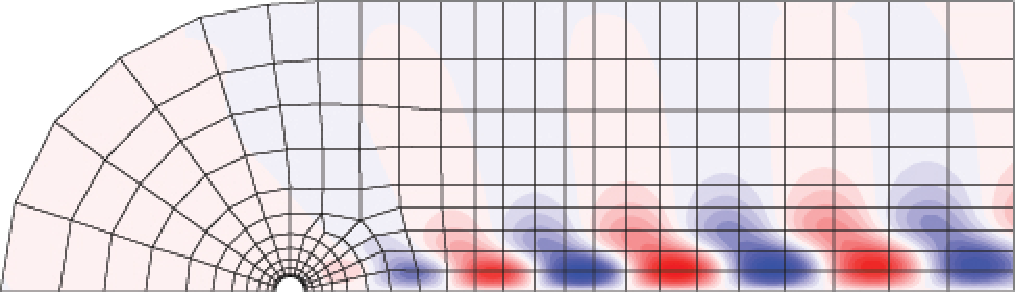
\includegraphics[width=0.425\textwidth]{Re50_eig0_u_mesh.pdf} &
(b) &

\includegraphics[width=0.425\textwidth]{Re50_eig1_u.pdf} \\
&

\includegraphics[width=0.425\textwidth]{Re50_eig0_v.pdf} &
&

\includegraphics[width=0.425\textwidth]{Re50_eig1_v.pdf}
\end{tabular}
\end{center}
\caption{Contour plots of (upper) $u'$ velocity component and (lower)
  $v'$ velocity component of leading eigenmodes (a) 0 and (b) 1 of
  \twod\ flow past a circular cylinder at $\Rey=50$.}
\label{fig.semimodes}
\end{figure}

We go ahead and re-run the analysis for $\Rey=40$ (remembering to edit
the session file appropriately), resulting in
{\small
\begin{verbatim}
-- Iteration = 46, H(k+1, k) = 0.55706
EV  Magnitude   Angle       Growth      Frequency   Residual
 0  9.4477e-01  1.5391e+00 -2.8406e-02  7.6953e-01  6.5654e-07
 1  9.4477e-01 -1.5391e+00 -2.8406e-02 -7.6953e-01  6.5654e-07
 2  7.2675e-01  1.6334e+00 -1.5959e-01  8.1669e-01  2.9849e-03
 3  7.2675e-01 -1.6334e+00 -1.5959e-01 -8.1669e-01  2.9849e-03
 4  7.4011e-01  1.3563e+00 -1.5048e-01  6.7816e-01  4.0655e-03
 5  7.4011e-01 -1.3563e+00 -1.5048e-01 -6.7816e-01  4.0655e-03
 6  6.6511e-01  1.1237e+00 -2.0390e-01  5.6186e-01  1.6093e-02
 7  6.6511e-01 -1.1237e+00 -2.0390e-01 -5.6186e-01  1.6093e-02
 8  6.1827e-01  4.0307e-01 -2.4041e-01  2.0153e-01  3.0627e-01
 9  6.1827e-01 -4.0307e-01 -2.4041e-01 -2.0153e-01  3.0627e-01
dog: converged, writing 2 eigenvectors.
\end{verbatim}
}
\noindent
We see that the flow at $\Rey=40$ is stable, as expected.

By linear interpolation (which is probably less than adequate given
the large spread in $\Rey$) we can estimate $\Rey_c=46.144$, at which
value the interpolated circular frequency is $\omega=0.77974$, so that
the critical Strouhal number estimate is
$\Str_c=(2\pi)^{-1}0.77974=0.12410$.  These values are in quite good
agreement with those provided by \citet{jack87} ($\Rey_c=46.184$,
$\Str_c=0.1384$) and \citet{kumi06} ($\Rey_c=47.786$, $\Str_c=0.12441$
at the present blockage ratio of 1/20).  Possible sources of
discrepancy: effect of coarse linear interpolation for critical values
(try another solution closer to critical $\Rey$); comparatively large
blockage ratio of our domain \citep[see][regarding
  sensitivity]{kumi06}; base flows not converged to steady state (run
them longer); lack of resolution; small errors in the cited studies.

%=============================================================================
\section{Steady \twod\ flow in a stenosed tube
\protect\footnote{Input files for this example are supplied in
  \texttt{dog/testcases/Steady/stenosis}.}  }
\label{sec.sten3D}

A stenosis is a partial blockage or localised contraction in an
otherwise parallel walled geometry.  The basic geometry is tubular and
so we solve this problem using cylindrical coordinates.  The base flow
is 2D2C, steady in time in this case, and the least stable eigenmodes
are 3D3C, occurring in aziumuthal wavenumber $k=1$, see
\citet{shbl05}. This mode shape promotes attachment of the jet which
issues from the stenosis throat to the wall of the tube
downstream. With the contraction geometry we will consider,
$\Rey_c=722$ (based on upstream pipe diameter $D$ and area-averaged
flow speed $\bar{u}_m$), but we will here study a stable case at
$\Rey=500$, for which resolution and domain extent requirements are
less, speeding up our analysis.  According to the inset of figure~5,
\citet{shbl05}, the leading eigenvalue is real and negative,
$\lambda\approx0.053$.

%-----------------------------------------------------------------------------
\subsection{Geometry and base flow}

The solution domain geometry is shown in figure~\ref{fig.sten}.  As is
standard for cylindrical coordinate system solutions, the geometry is
represented in the `meridional semiplane' and in this case the lower
bound is the axis of the coordinate system.

\begin{figure}
\begin{center}
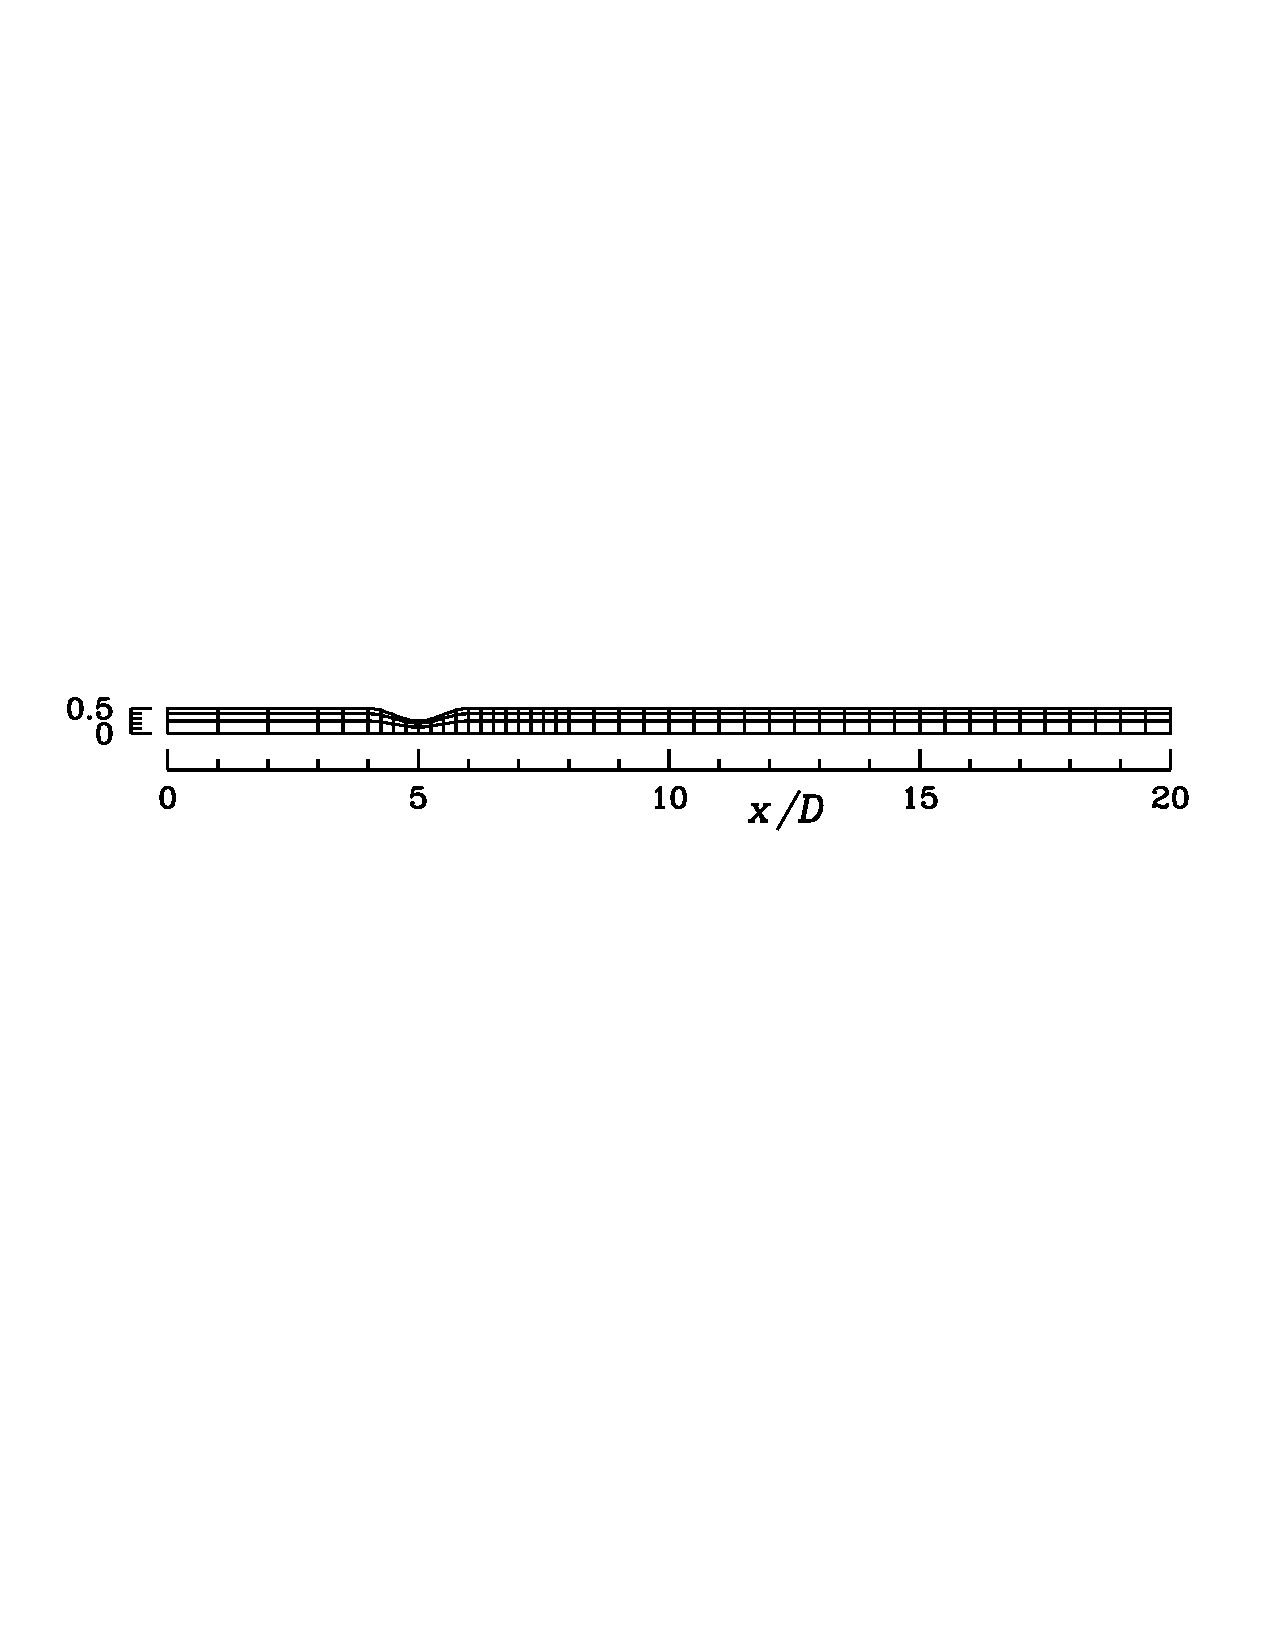
\includegraphics[width=\textwidth]{stenosismesh}
\end{center}
\caption{Spectral element mesh of the meridional semiplane for flow in
  a stenosed tube.}
\label{fig.sten}
\end{figure}

The session file for the base flow, \verb+stenosis-base+, is given
below. Note that the outer boundary near the stenosis is a smooth
curve which is represented as a spline through points given in a
separate file, specified in the \verb+CURVES+ section (see \S\,3.2.1
of the \Semtex\ user guide).

{\small
\begin{verbatim}
<TOKENS>
  CYLINDRICAL = 1
  KINVIS      = 1/500
  D_T         = 0.001
  T_MAX       = 500
  N_STEP      = int(T_MAX/D_T)
  N_P         = 7
  BETA        = 1
</TOKENS>

<FIELDS NUMBER=3>
  u  v  p
</FIELDS>

<GROUPS NUMBER=4>
  1  w  wall
  2  v  velocity
  3  o  exit
  4  a  axis
</GROUPS>

<BCS NUMBER=4>
1  w  3
  <D> u = 0.0 </D>
  <D> v = 0.0 </D>
  <H> p       </H>
2  v  3
  <D> u = 2*(1-4*y^2) </D>
  <D> v = 0.0         </D>
  <H> p               </H>
3  o  3
  <N> u = 0.0 </N>
  <N> v = 0.0 </N>
  <D> p = 0.0 </D>
4  a  3
  <A> u </A>
  <A> v </A> 
  <A> p </A>
</BCS>

<HISTORY NUMBER=3>
	 1	6	0.45	0
	 2	10	0.45	0
	 3	19	0.45	0
</HISTORY>

<NODES NUMBER=184>
 1 0.000000 0.000000 0.000000 
 2 1.000000 0.000000 0.000000 
 3 2.000000 0.000000 0.000000 
 ..
 ..
 184 20.000000 0.500000 0.000000 
</NODES>

<ELEMENTS NUMBER=135>
    1	<Q>    1    2   48   47    </Q>
    2	<Q>    2    3   49   48    </Q>
    3	<Q>    3    4   50   49    </Q>
    ..
    ..
  135	<Q>  137  138  184  183    </Q>
</ELEMENTS>

<SURFACES NUMBER=96>
    1    1    1    <B> a </B>
    2    2    1    <B> a </B>
    3    3    1    <B> a </B>
    ..
    ..
   45   45    1    <B> a </B>

   46   45    2    <B> o </B>
   47   90    2    <B> o </B>
   48  135    2    <B> o </B>

   49  135    3    <B> w </B>
   50  134    3    <B> w </B>
   51  133    3    <B> w </B>
   ..
   ..
   93   91    3    <B> w </B>

   94   91    4    <B> v </B>
   95   46    4    <B> v </B>
   96    1    4    <B> v </B>
</SURFACES>

<CURVES NUMBER=8>
 1	 96	3	<SPLINE> stenosis-upper.geom </SPLINE>	
 2	 97	3	<SPLINE> stenosis-upper.geom </SPLINE>	
 3	 98	3	<SPLINE> stenosis-upper.geom </SPLINE>
 ..
 ..	
 8	 103	3	<SPLINE> stenosis-upper.geom </SPLINE>	
</CURVES>
\end{verbatim}
}

We have chosen to run the base flow for 500 time units, and have made
a set of history points located near the recirculation zone to check
that the base flow is steady.  The timeseries from these points,
available in \verb+stenosis-base.his+ after running \verb+dns+, are
shown in figure~\ref{fig.stenhis}.  While a finer-scale examination is
advisable, we'll accept that the base flow is likely to be close to
the asymptotic steady state at the end of this simulation.

\begin{figure}
\begin{center}
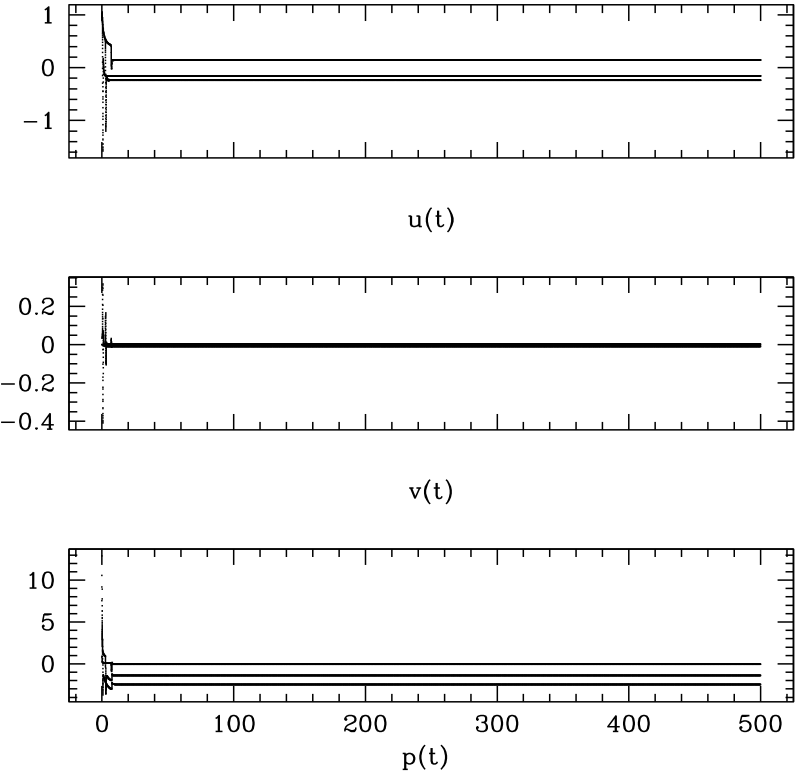
\includegraphics[width=0.55\textwidth]{StenBaseHis}
\end{center}
\caption{Time series from three base flow history points in the
  simulation of the steady flow in a stenotic geometry. We note that
  two of the points are within the recirculation zone, and one is
  outside.  There seem to be no significant dynamics after
  $t\approx10$ and we will accept the final flow as being close to its
  steady state outcome.}
\label{fig.stenhis}
\end{figure}

%-----------------------------------------------------------------------------
\subsection{Stability analysis}

Again we modify the base flow session file in order to produce one for
stability analysis, which we will call \verb+stenosis+.  The
significant differences between this and the base flow session file
are shown below.  
{\small
\begin{verbatim}
<TOKENS>
  N_BASE      = 2
  N_SLICE     = 1
  CYLINDRICAL = 1
  N_Z         = 1
  BETA        = 1
  KINVIS      = 1/500
  D_T         = 0.001
  T_MAX       = 0.5
  N_STEP      = int(T_MAX/D_T)
  N_P         = 7
</TOKENS>

<FIELDS NUMBER=4>
  u  v  w  p
</FIELDS>

<BCS NUMBER=4>
1  w  4
  <D> u = 0.0 </D>
  <D> v = 0.0 </D>
  <D> w = 0.0 </D>
  <H> p       </H>
2  v  4
  <D> u = 0.0 </D>
  <D> v = 0.0 </D>
  <D> w = 0.0 </D>
  <H> p       </H>
3  o  4
  <N> u = 0.0 </N>
  <N> v = 0.0 </N>
  <N> w = 0.0 </N>
  <D> p = 0.0 </D>
4  a  4
  <A> u </A>
  <A> v </A> 
  <A> w </A> 
  <A> p </A>
</BCS>
\end{verbatim}
}
\noindent
In the \verb+TOKENS+ section we have added \verb+N_BASE=2+ and
\verb+N_SLICE=1+ as befits a steady, \twoc\ base flow.  We are
carrying out the analysis in azimuthal wavenumber $k\equiv\beta=1$ and
have set this with \verb+BETA=1+. The instability mode is of
`half-complex' type, with the restricted symmetry
$u'=\hat{u}'\cos(k\theta), v'=\hat{v}'\cos(k\theta),
w'=-\hat{u}'\sin(k\theta), p'=\hat{p}'\cos(k\theta)$, so that we only
need \verb+N_Z=1+.  The integration time $\tau=0.5$ is set with
\verb+T_MAX=0.5+ and \verb+N_STEP=int(T_MAX/D_T)+.

In the \verb+FIELDS+ section there are now a total of four fields
(recall that there were only three for the base flow), the first three
of which are velocity components.  Since we have set \verb+BETA=1+ as
well, we will have 3D3C eigenmodes.

In the \verb+BCS+ section, first note that we have to add a condition
to each subsection for the new velocity component, $w$, that was not
present in the base flow. Second, observe that at the inflow (the
second, \verb+v+-tagged subsection, we have set the perturbation field
to zero.

Now we are ready to run the stability analysis:
\begin{verbatim}
[mec-aquila]$ ln -sf stenosis-base.fld stenosis.bse; \
enumerate -O3 stenosis > stenosis.num; \
dog -k 8 -n 1 -m 100 -t 1e-8 stenosis > /dev/null &
tail -f stenosis.evl
\end{verbatim}
which should terminate with
{\small
\begin{verbatim}
-- Iteration = 71, H(k+1, k) = 0.345441
EV  Magnitude   Angle       Growth      Frequency   Residual
 0  9.7370e-01  0.0000e+00 -5.3306e-02  0.0000e+00  8.6888e-09
 1  7.6511e-01  1.6542e-01 -5.3546e-01  3.3083e-01  8.1313e-04
 2  7.6511e-01 -1.6542e-01 -5.3546e-01 -3.3083e-01  8.1313e-04
 3  5.3337e-01  7.0926e-01 -1.2571e+00  1.4185e+00  2.0783e-02
 4  5.3337e-01 -7.0926e-01 -1.2571e+00 -1.4185e+00  2.0783e-02
 5  7.4996e-01  1.7543e+00 -5.7548e-01  3.5086e+00  6.7510e-02
 6  7.4996e-01 -1.7543e+00 -5.7548e-01 -3.5086e+00  6.7510e-02
 7  5.9257e-01  0.0000e+00 -1.0466e+00  0.0000e+00  1.3208e-01
dog: converged, writing 1 eigenvectors.
\end{verbatim}
}\noindent We see that the leading eigenvalue is real and stable;
$\lambda_0=-5.3306\times10^{-2}$, close the value we had expected.


%-----------------------------------------------------------------------------
\subsection{Cross-check: growth rates via DNS}
\label{sec.check}

\begin{figure}
\begin{center}
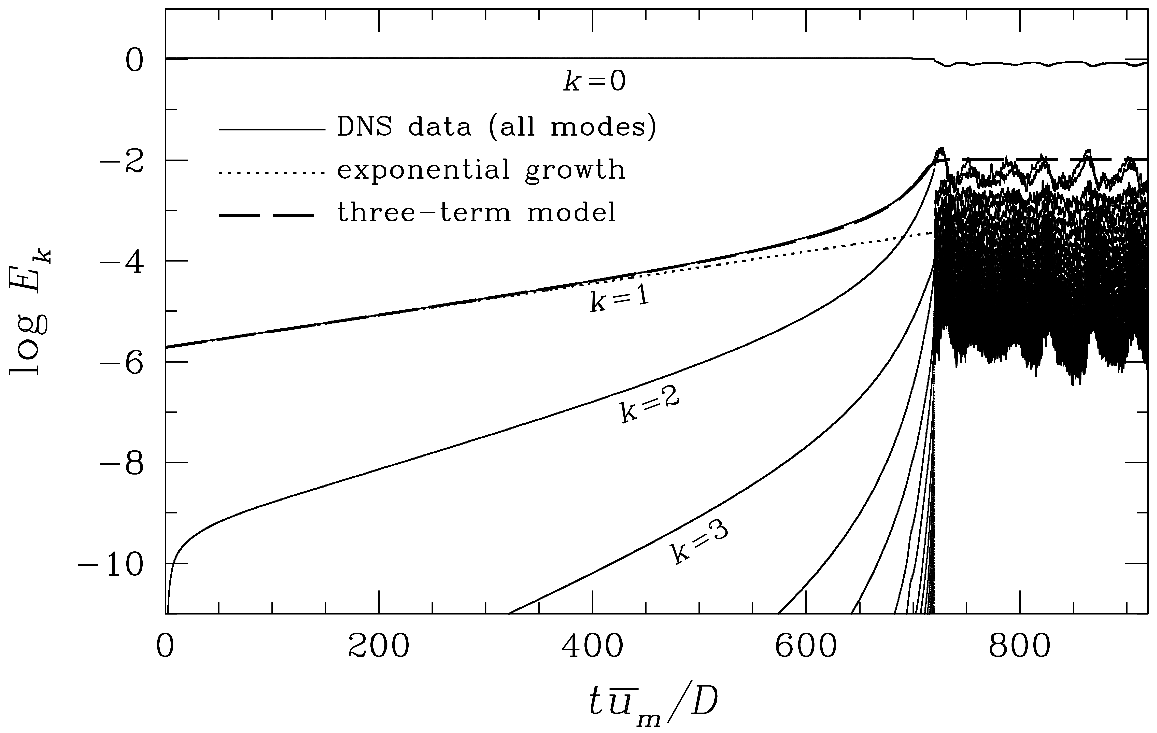
\includegraphics[width=0.65\textwidth]{StenGrow}
\end{center}
\caption{DNS study of growth rate for an unstable steady stenotic flow
  at $\Rey=750$, see \citet{shbl05} and the discussion in
  \S\,\ref{sec.check} of the present work.  }
\label{fig.stengrow}
\end{figure}

A good test of stability analysis is that the weakly nonlinear
evolution of a DNS study restarted using a linear combination of the
base flow and a small amount of the eigenmode exhibits the same
disturbance growth rate as predicted by linear stability analysis.  The
restart condition can be obtained using \Dog's \verb|combine| utility,
which produces a physical-space restart file from a base flow and an
eigenmode.  The number of $z$-planes in the restart file outcome is
the minimal number required to contain both modes in physical space.
Typically, for a \threed\ disturbance, this number of planes is four,
and in order to produce something more suitable for use with
\verb|dns| you will need to project out to a greater number using
\Semtex's project utility.  For example:
\begin{verbatim}
$ combine -r 1-e4 stenosis.bse stenosis.eig.0 | project -z 64 > stenosis.rst
\end{verbatim}

One can then check the growth of energy in the disturbance as obtained
using DNS.  Since energy is the square of velocity, this growth rate
should be very close to twice the value of the leading eigenmode.  See
for example the discussion in \S\,5.3 of \citet{shbl05}, and a version
of figure~6 from that work, reproduced here as
figure\,\ref{fig.stengrow}.  The growth rate of the disturbance can be
estimated at early times (while the disturbance growth is still
clearly exponential) as
\begin{equation}
  \sigma_\text{est} = \frac{\Delta \ln(E_{k=1})}{2\Delta t};
\end{equation}
if all is well, this value should be quite similar to the leading
eigenvalue.



%%%%%%%%%%%%%%%%%%%%%%%%%%%%%%%%%%%%%%%%%%%%%%%%%%%%%%%%%%%%%%%%%%%%%%%%%%%%%%
\chapter{Stability analysis of time-periodic flows}
\label{ch.floquet}

A few new issues arise in dealing with temporal Floquet analysis: (a)
the base flow must be periodic and (b) we must provide enough
time-slices of it for an adequate reconstruction to be possible.  In
order to check periodicity, one can examine phase-space plots of
velocity components in order to ensure they have closed to make limit
cycles, but also it is advisable to check that the frequency of
oscillation has in fact converged to the same value at different
history points.  We note that DFT-based Fourier analysis is generally
NOT a good choice for checking the base flow frequency at different
points and that tools based in the time domain \citep[\eg
  zero-crossing analysis, see chapter~8 of][]{newland93} are to be
preferred. As to the number of time-slices required for accurate
reconstruction, a convergence analysis is really the only option.
Also I suggest you read the caveats issued in \S\,4.1 of
\citet{bbs08b}.

%=============================================================================
\section{Time-periodic flow past a circular cylinder
\protect\footnote{Input files for this example are supplied in
  \texttt{dog/testcases/Floquet/cylinder}.}  }
\label{sec.cyl2d}

Here we deal with Floquet analysis of a \twod\ time-periodic flow past
a circular cylinder, studied in detail by \citet{bah96}.  We will
examine near-critical behaviour for Mode~A, which \citeauthor{bah96}
report has $\Rey_c=188.5$ at $\beta_c=1.585$.  They used 32
time-slices per base flow period for their Fourier-based
reconstruction of the base flow.

%-----------------------------------------------------------------------------
\subsection{Geometry and base flow}

The mesh developed for the problem is shown in
figure~\ref{fig.cylinder}.  It has 218 elements, an inflow length
$L_i=15D$, outflow length $L_o=25D$ and semi-width $L_h=20$, all of
which are comparable to the production geometry $M_2$ used by
\citet{bah96}, though their cross-flow blockage was somewhat lower
since they had $L_h=22D$.

\begin{figure}
\begin{center}
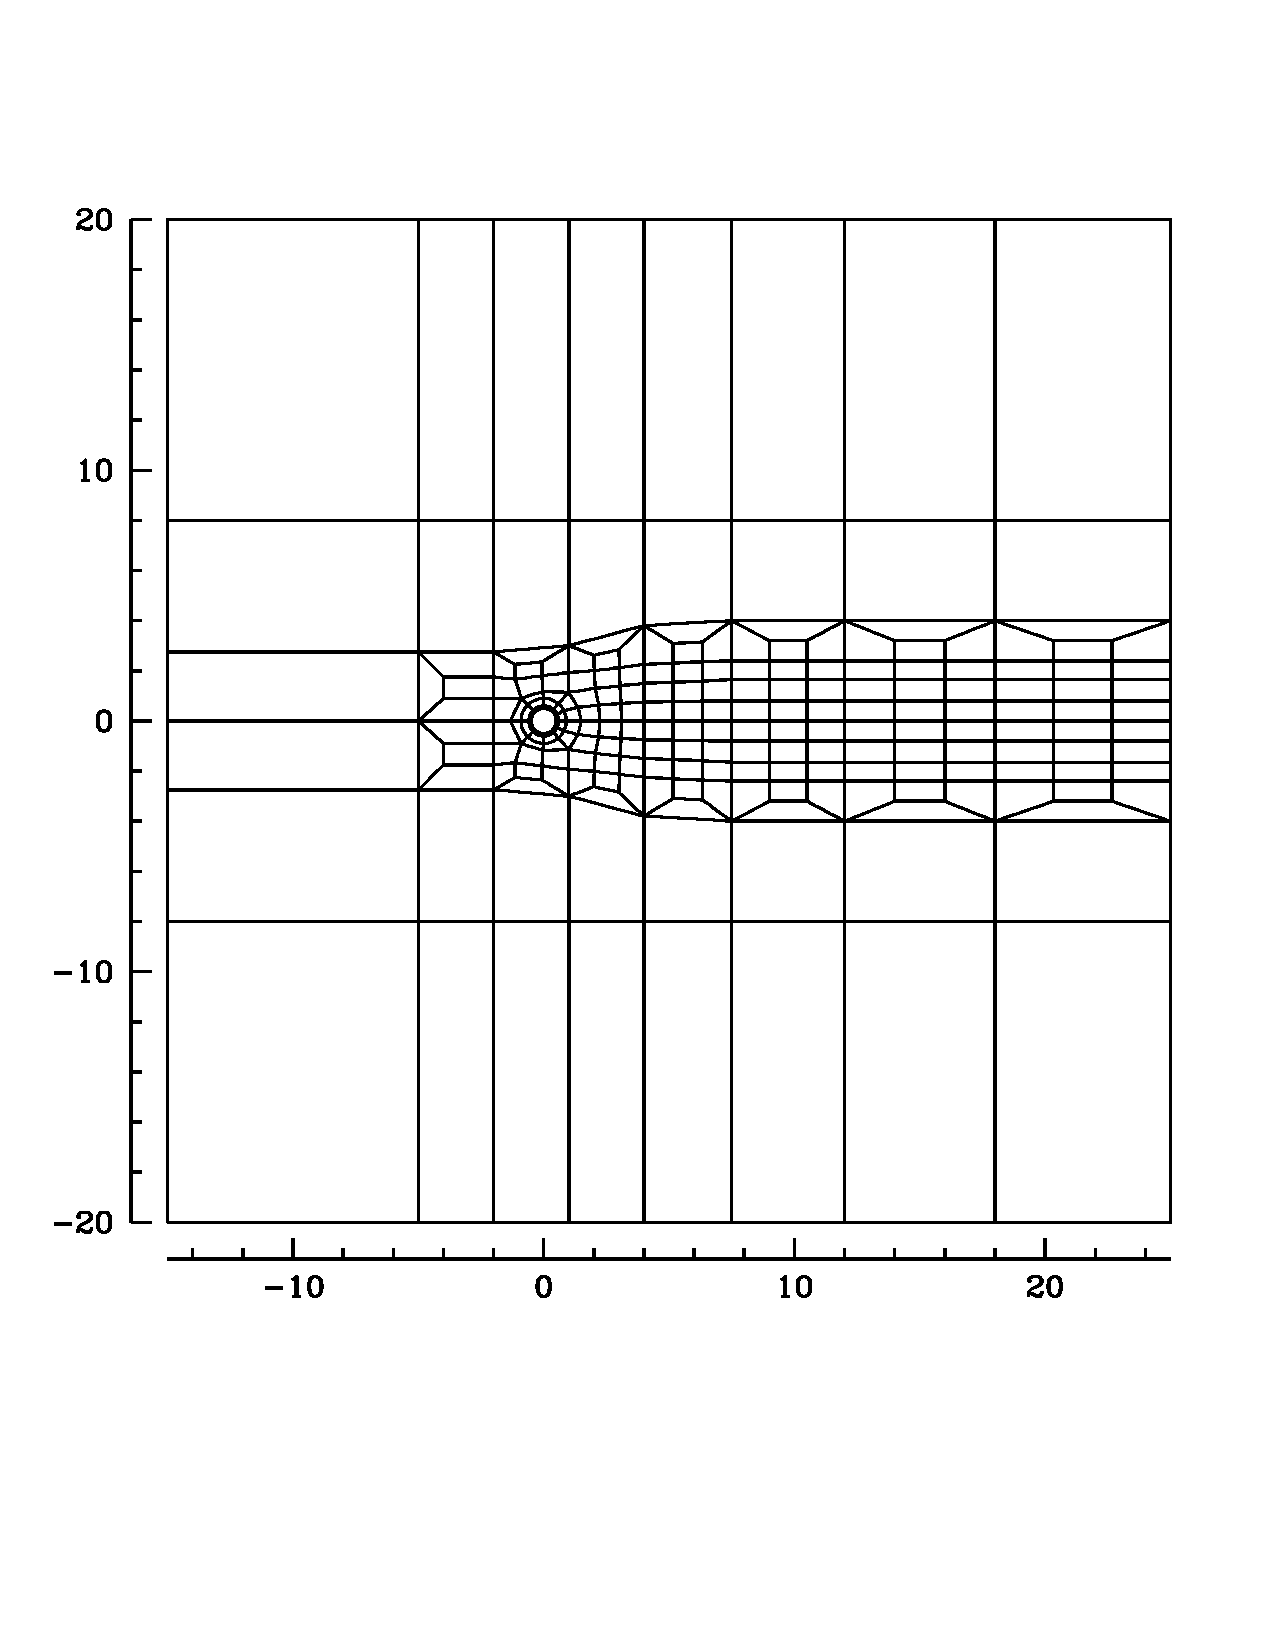
\includegraphics[width=0.6\textwidth]{m32_2D_mesh}
\end{center}
\caption{Spectral element mesh for Floquet analysis of flow past a
  circular cylinder.}
\label{fig.cylinder}
\end{figure}

The session file (\verb+m32-base+) used to compute the base flow is
shown below.  Some of the \verb+TOKENS+ correspond to our initial
guesses, a point we will return to below.

{\small
\begin{verbatim}
<TOKENS>
  PERIOD    = 5.0
  STEP_PER  = 1024

  N_STEP    = 200*STEP_PER
  D_T       = (PERIOD/STEP_PER)
  IO_FLD    = STEP_PER/32
  CHKPOINT  = 1

  N_P       = 8
  Re        = 188.5
  KINVIS    = 1/Re
</TOKENS>

<HISTORY NUMBER=3>
  1  2.0   0.0  0.0
  2  10.0  0.0  0.0
  3  20.0  0.0  0.0
</HISTORY>

<FIELDS NUMBER=3>
  u  v  p
</FIELDS>

<GROUPS NUMBER=3>
  1  v  velocity
  2  w  wall
  3  o  exit
</GROUPS>

<BCS NUMBER=3>
  1  v  3
    <D>  u = 1.0  </D>
    <D>  v = 0.0  </D>
    <H>  p        </H>
  2  w  3
    <D>  u = 0.0  </D>
    <D>  v = 0.0  </D>
    <H>  p        </H>
  3  o  3
    <N>  u = 0.0  </N>
    <N>  v = 0.0  </N>
    <D>  p = 0.0  </D>
</BCS>

<NODES NUMBER=286>
    1        0.5           0         0
    2    0.44721     0.22361         0
    3    0.32139     0.38302         0
   ..
   ..
  286         25         -20         0
</NODES>

<ELEMENTS NUMBER=218>
 1	<Q>  1	11	12	2	</Q>
 2	<Q>  2	12	13	3	</Q>
 3	<Q>  3	13	14	4	</Q>
 ..
 ..
218	<Q>  278	279	49	277	</Q>
</ELEMENTS>

<SURFACES NUMBER=44>
	1	199	3	<B>	v	</B>
	2	201	3	<B>	v	</B>
	3	203	3	<B>	v	</B>
        ..
        ..
	22	212	1	<B>	v	</B>

	23	199	2	<B>	o	</B>
	24	183	2	<B>	o	</B>
	25	151	2	<B>	o	</B>
        ..
        ..
	34	200	2	<B>	o	</B>

	35	1	4	<B>	w	</B>
	36	2	4	<B>	w	</B>
	37	3	4	<B>	w	</B>
        ..
        ..
	44	10	4	<B>	w	</B>
</SURFACES>

<CURVES NUMBER=50>
 1	 1	4	<ARC>	-0.5	</ARC>
 2	 2	4	<ARC>	-0.5	</ARC>
 3	 3	4	<ARC>	-0.5	</ARC>
..
..
50	30	4	<ARC>	-0.9	</ARC>
</CURVES>
\end{verbatim}
}

Now we set about running and checking the base flow.  In the
\verb+TOKENS+ section we have guessed the final oscillation period to
be of order 5 time units (based on a Strouhal number of order 0.2,
typical for circular cylinders) and run for 200 periods (total time of
1000 units), hoping the base flow to become established and periodic
in this time span.  Note that we have included three history points at
various locations inside the wake.

\begin{verbatim}
[mec-aquila]$ enumerate -O3 m32-base > m32-base.num ; \
dns m32-base > /dev/null ; \
save m32-base
\end{verbatim}
\noindent
(\verb+save+ is a standard \Semtex\ shell script.) Next we visually
examine the base flow history time series for $(U,V,P)$ and as a
phase-plane plot, as shown in figure~\ref{fig.shedding}.  Based on
this inspection, it is tempting to believe that the flow has reached
an asymptotic limit-cycle state and is suitable for use as a base
flow.  However, let us also check the periods associated with each of
the history points (for which we will use an up-crossing analysis
tool, not supplied).

\begin{figure}
\begin{center}
\begin{tabular}{cccc}
\raisebox{40ex}{(a)} &
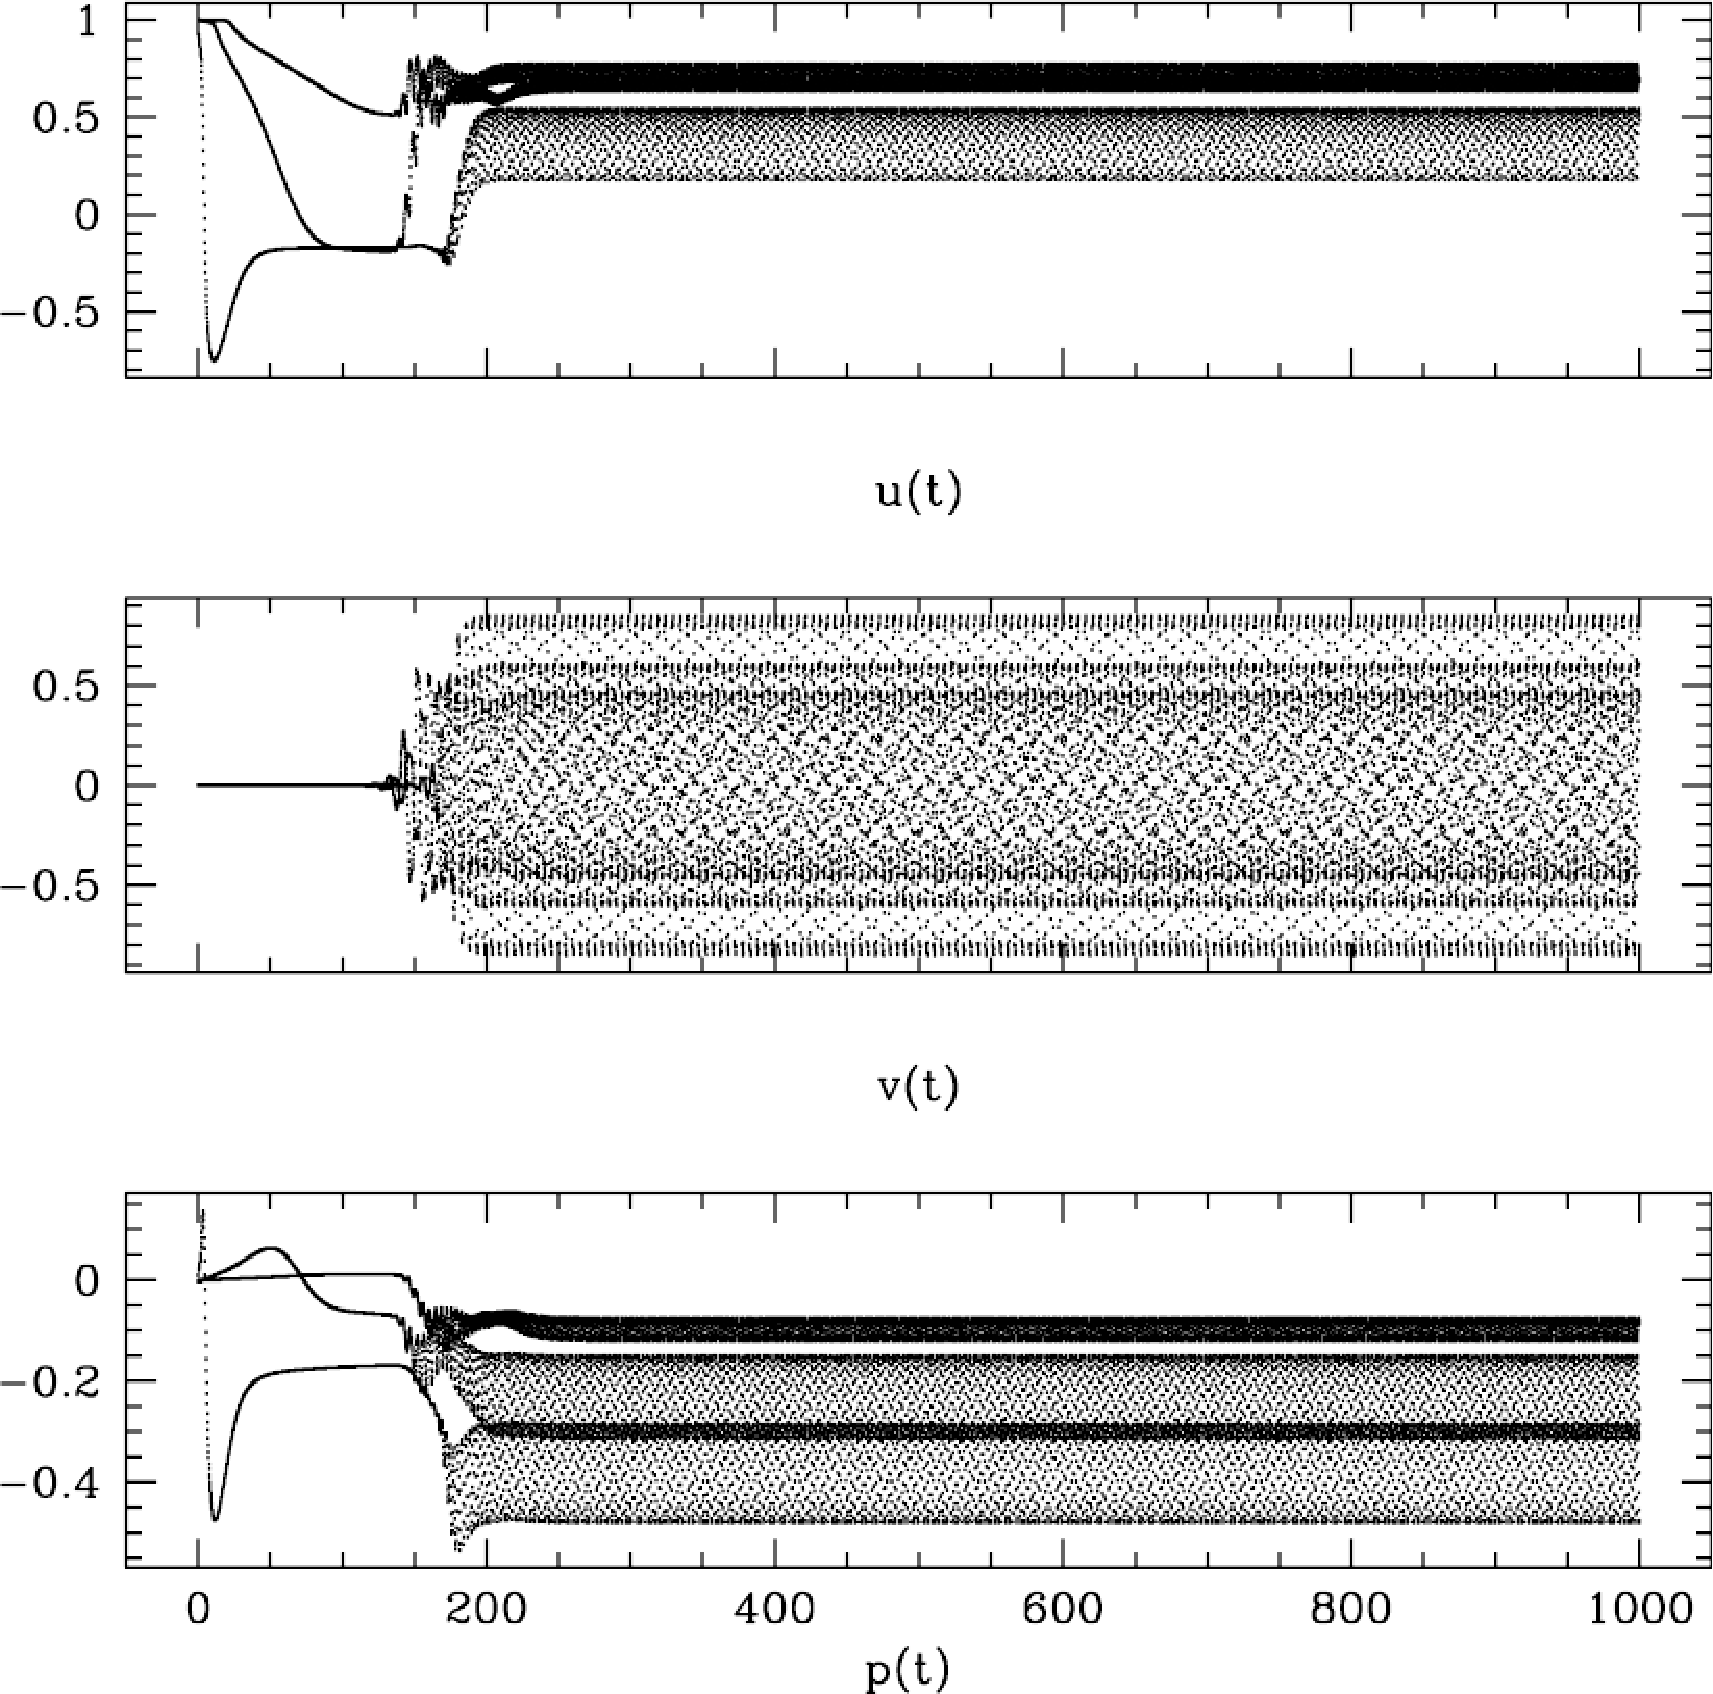
\includegraphics[width=0.45\textwidth]{base_his} &
\raisebox{40ex}{(b)} &
\raisebox{5ex}{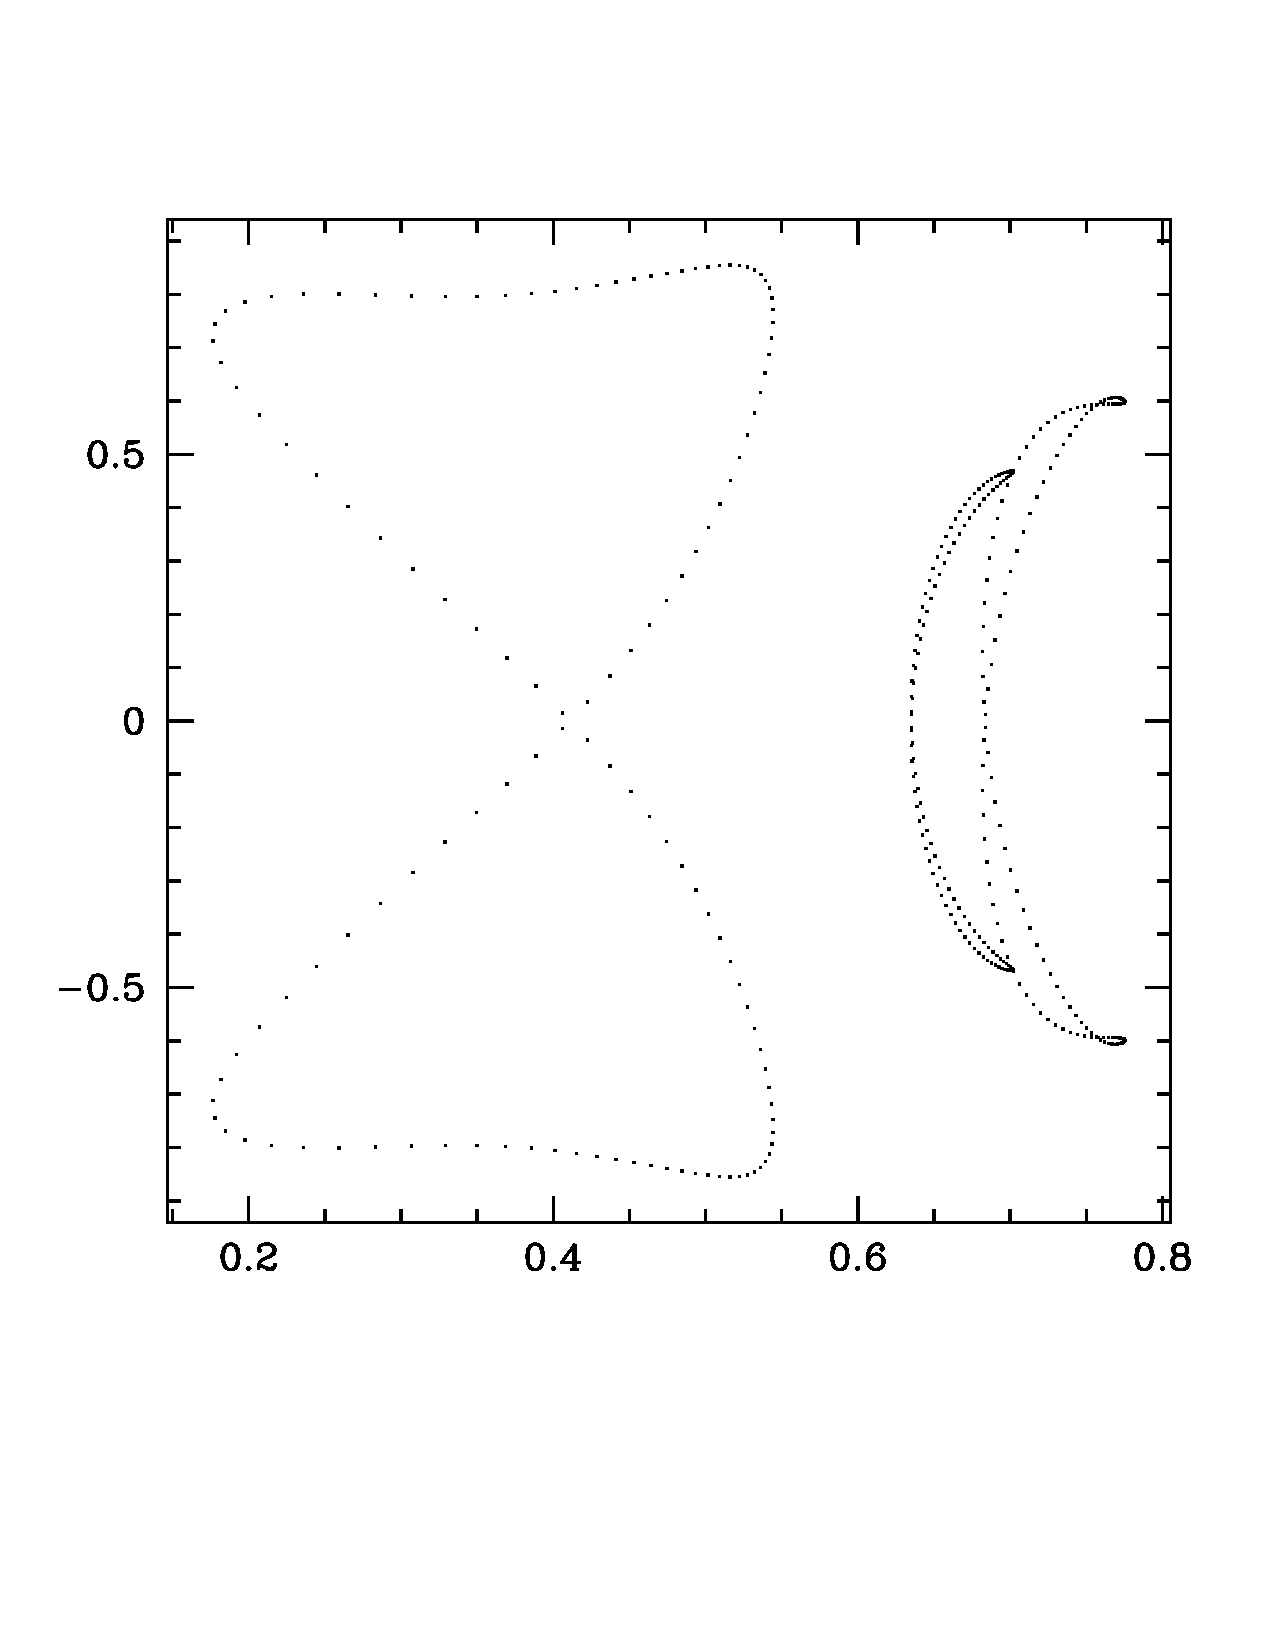
\includegraphics[width=0.4\textwidth]{limcyc}}
\end{tabular}
\end{center}
\caption{(a) History point time series for the first 1000 time units
  of simulation for circular cylinder base flow. (b) phase-plane plot
  of $U$ vs $V$ for final few shedding cycles.}
\label{fig.shedding}
\end{figure}

Analysis for $V$ velocity component, history point 1:
\begin{verbatim}
[mec-aquila]$ chop -s 1 -S 3 m32-base.his | slit -c 2,4 | upxf -v | tail -4 
9.8745e+02 1.9563e-01 1.8661e-01 -8.5490e-01 -7.6585e-01 8.5490e-01 7.6343e-01
9.9256e+02 1.9561e-01 1.8666e-01 -8.5491e-01 -7.6634e-01 8.5487e-01 7.6394e-01
9.9767e+02 1.9559e-01 1.8671e-01 -8.5488e-01 -7.6684e-01 8.5489e-01 7.6444e-01
averages:  frequency  1.8671e-01,        min -7.6684e-01,       max 7.6444e-01
\end{verbatim}

For history point 2:
\begin{verbatim}
[mec-aquila]$ chop -s 2 -S 3 m32-base.his | slit -c 2,4 | upxf -v | tail -4 
9.8679e+02 1.9557e-01 1.8657e-01 -6.0652e-01 -5.5939e-01 6.0653e-01 5.5733e-01
9.9190e+02 1.9557e-01 1.8662e-01 -6.0653e-01 -5.5966e-01 6.0653e-01 5.5760e-01
9.9701e+02 1.9559e-01 1.8667e-01 -6.0653e-01 -5.5992e-01 6.0652e-01 5.5788e-01
averages:  frequency  1.8667e-01,        min -5.5992e-01,       max 5.5788e-01
\end{verbatim}

For history point 3:
\begin{verbatim}
[mec-aquila]$ chop -s 3 -S 3 m32-base.his | slit -c 2,4 | upxf -v | tail -4 
9.8803e+02 1.9558e-01 1.9196e-01 -4.6848e-01 -4.2681e-01 4.6849e-01 4.2543e-01
9.9315e+02 1.9558e-01 1.9198e-01 -4.6849e-01 -4.2704e-01 4.6849e-01 4.2567e-01
9.9826e+02 1.9559e-01 1.9200e-01 -4.6849e-01 -4.2727e-01 4.6848e-01 4.2591e-01
averages:  frequency  1.9200e-01,        min -4.2727e-01,       max 4.2591e-01
\end{verbatim}

The relevant features in the above listings are the second columns,
which give the frequency (inverse period) for the final three cycles
found at each history point.  We can see that despite the fact that
the phase-plane plots in figure~\ref{fig.shedding} seem converged, the
frequencies are still slowly evolving\,---\,even though the final
values happen to be the same (0.19559).  So we will resubmit the base
flow for another 1000 time units.\footnote{This might seem like
  overkill, but it turns out that a Floquet analysis employing the
  base flow at this stage of evolution would be moderately in error.
  (Try it out for yourself.)}

After re-running \verb+dns+ we re-make our crossing analysis and find
(only reproducing data for the first point, since the other two are
identical):
\begin{verbatim}
[mec-aquila]$ dns m32-base > /dev/null; save m32-base
[mec-aquila]$ chop -s 1 -S 3 m32-base.his | slit -c 2,4 | upxf -v | tail -4 
2.0099e+03 1.9560e-01 1.9560e-01 -8.5487e-01 -8.5487e-01 8.5487e-01 8.5487e-01
2.0151e+03 1.9560e-01 1.9560e-01 -8.5487e-01 -8.5487e-01 8.5487e-01 8.5487e-01
2.0202e+03 1.9560e-01 1.9560e-01 -8.5487e-01 -8.5487e-01 8.5487e-01 8.5487e-01
averages:  frequency  1.9560e-01,        min -8.5487e-01,       max 8.5487e-01
\end{verbatim}
\noindent We find that the frequency has now converged to a value of
0.19560, the same for all history points.  Now we are in a position to
compute the time-slices required for the base flow and alter the
\verb+TOKENS+ section accordingly:
{\small
\begin{verbatim}
<TOKENS>
  FREQ        = 0.19560
  BASE_PERIOD = 1.0/FREQ
  STEP_PER    = 1024
  N_STEP      = 1*STEP_PER
  D_T         = (BASE_PERIOD/STEP_PER)
  IO_FLD      = STEP_PER/32
  CHKPOINT    = 0
  N_P         = 8
  Re          = 188.5
  KINVIS      = 1/Re
  IO_CFL      = 32
  IO_HIS      = 8
</TOKENS>
\end{verbatim}
}
\noindent
The most significant modifications here are used to (a) set the total
integration time to one base flow period (b) ensure that all 32
field dumps are written to the output file (via \verb+CHKPOINT=0+).
Our time step is very similar to what was chosen for the set-up
phases.  While we have used the token \verb+BASE_PERIOD+ here, the
name is not significant to \verb+dns+. The same is true for these
other tokens: \verb+FREQ+, \verb+STEP_PER+, \verb+Re+.
\begin{verbatim}
[mec-aquila]$ dns m32-base > /dev/null; ln -s m32-base.fld m32.bse
\end{verbatim}
\noindent Here we have linked the outcome so that it will serve as a
base flow file for Floquet analysis with session file \verb+m32+.  We
can easily (and should) check the number of field dumps in
\verb+m32.bse+:
\begin{verbatim}
[mec-aquila]$ convert m32.bse | grep -c Session
32
\end{verbatim}

%-----------------------------------------------------------------------------
\subsection{Floquet analysis}

Below we see an extract from the listing for our \Dog\ session file,
\verb+m32+, showing the parts that differ from the base flow's session
file.  Note that since the base flow is 2D2C and the Floquet modes are
3D3C, we need to add in boundary conditions for the $w$ velocity
component. And that since the conditions are satisfied for a
`half-complex' mode, we only need to set \verb+N_Z=1+.

{\small
\begin{verbatim}
<FIELDS NUMBER=4>
  u  v  w  p
</FIELDS>

<TOKENS>
  FREQ        = 0.19560
  BASE_PERIOD = 1.0/FREQ

  STEPS_P     = 1024
  N_STEP      = STEPS_P
  D_T         = BASE_PERIOD/STEPS_P

  N_P         = 8
  N_Z         = 1

  N_SLICE     = 32
  N_BASE      = 2

  IO_FLD      = STEPS_P
  IO_HIS      = 16
  IO_CFL      = 20

  BETA        = 1.585
  Re          = 188.5
  KINVIS      = 1.0/Re
</TOKENS>

<BASE_HIST NUMBER=3>
  1  2.0   0.0  0.0
  2  10.0  0.0  0.0
  3  20.0  0.0  0.0
</BASE_HIST>

<GROUPS NUMBER=3>
  1  v  velocity
  2  w  wall
  3  o  exit
</GROUPS>

<BCS NUMBER=3>
  1  v  4
    <D>  u = 0.0  </D>
    <D>  v = 0.0  </D>
    <D>  w = 0.0  </D>
    <H>  p        </H>
  2  w  4
    <D>  u = 0.0  </D>
    <D>  v = 0.0  </D>
    <D>  w = 0.0  </D>
    <H>  p        </H>
  3  o  4
    <N>  u = 0.0  </N>
    <N>  v = 0.0  </N>
    <N>  w = 0.0  </N>
    <D>  p = 0.0  </D>
</BCS>
\end{verbatim}
}
\noindent
The only substantive difference to our usage for steady flows is
setting \verb+N_SLICE=32+, which should be the number of time slices
present in the base flow (pre-declaring it allows us to allocate
storage prior to parsing the base flow file, but the correspondence is
subsequently checked within the code). Declaration of the base flow
period using the token \verb+BASE_PERIOD+ is optional (since this
would otherwise be computed from the base flow file), but including it
here enables us to set the time step \verb+D_T+ such that an integer
number of time steps occur each period.

Note the inclusion of (optional) \texttt{BASE\_HIST} section to
monitor base flow reconstruction from time slices, see
\S\,\ref{sec.specific}.  (In the analysis below, we have not
actually examined the \verb+m32.bhs+ file to check this
reconstruction, but it can be a useful diagnostic aid.)

So now we are ready to carry out the analysis.
\begin{verbatim}
[mec-aquila]$ enumerate -O3 m32 > m32.num ;\
dog -k 21 -n 1 -m 200 m32 > /dev/null &
tail -f m32.evl
\end{verbatim}
\noindent producing
{\small
\begin{verbatim}
-- Iteration = 31, H(k+1, k) = 0.493569
EV  Magnitude   Angle       Growth      Frequency   Residual
 0  9.9525e-01  0.0000e+00 -9.3136e-04  0.0000e+00  5.4271e-07
 1  6.7921e-01  1.5110e+00 -7.5663e-02  2.9555e-01  1.1243e-01
 2  6.7921e-01 -1.5110e+00 -7.5663e-02 -2.9555e-01  1.1243e-01
 3  6.5767e-01  2.6597e+00 -8.1967e-02  5.2025e-01  1.1926e-01
 4  6.5767e-01 -2.6597e+00 -8.1967e-02 -5.2025e-01  1.1926e-01
..
..
19  5.1720e-01  2.6095e+00 -1.2896e-01  5.1043e-01  3.5197e-01
20  5.1720e-01 -2.6095e+00 -1.2896e-01 -5.1043e-01  3.5197e-01
dog: converged, writing 1 eigenvectors.
\end{verbatim}
}
\noindent
Our leading Floquet multiplier estimate is $\mu_0=0.99525$, slightly
lower than $\mu=1$ predicted by \cite{bah96}, but we have employed a
slightly different cross-flow domain extent, and our results may also
change slightly as we increase resolution. As they also found, it
seems the next eigenvalue is of complex-conjugate type, giving rise to
a \qp\ mode \citep{bllo03b}.


%-----------------------------------------------------------------------------
\subsection{Getting a \threed\ eigenmode into physical space}

To get a \threed\ eigenmode from Fourier space into physical space
for viewing, use the \verb|combine| utility.\footnote{
This utility will also serve to combine a perturbation with a base
flow for subsequent evolution via \texttt{dns}.  In that case the first
file argument to combine would be (one time slice of) the base
flow. Here we just get the mode alone into physical space for
examination, in which case the eigenmode file is used as a dummy input
and \texttt{-r 0} specifies we are just dealing with the mode.}

\begin{verbatim}
[mec-aquila]$ combine -b 1.585 -r 0 m32.eig.0 m32.eig.0 | \
project -z 32 > m32_z32.eig.0
\end{verbatim}

In the above, we have also used the \Semtex\ \verb+project+ utility to
project the mode out from the minimum required number of $z$-planes
(4) to 32 in order to get a smoother-looking representation.  Finally
we could create a \Tecplot\ input file, like this:

\begin{verbatim}
[mec-aquila]$ meshpr -z 32 m32 | sem2tec m32_z32.eig.0
\end{verbatim}
\noindent which would produce \verb+m32_z32.eig.0.plt+.  We show an
image of the Floquet mode (visualised with \texttt{sview}) in
figure~\ref{fig.flok}.

\begin{figure}
\begin{center}
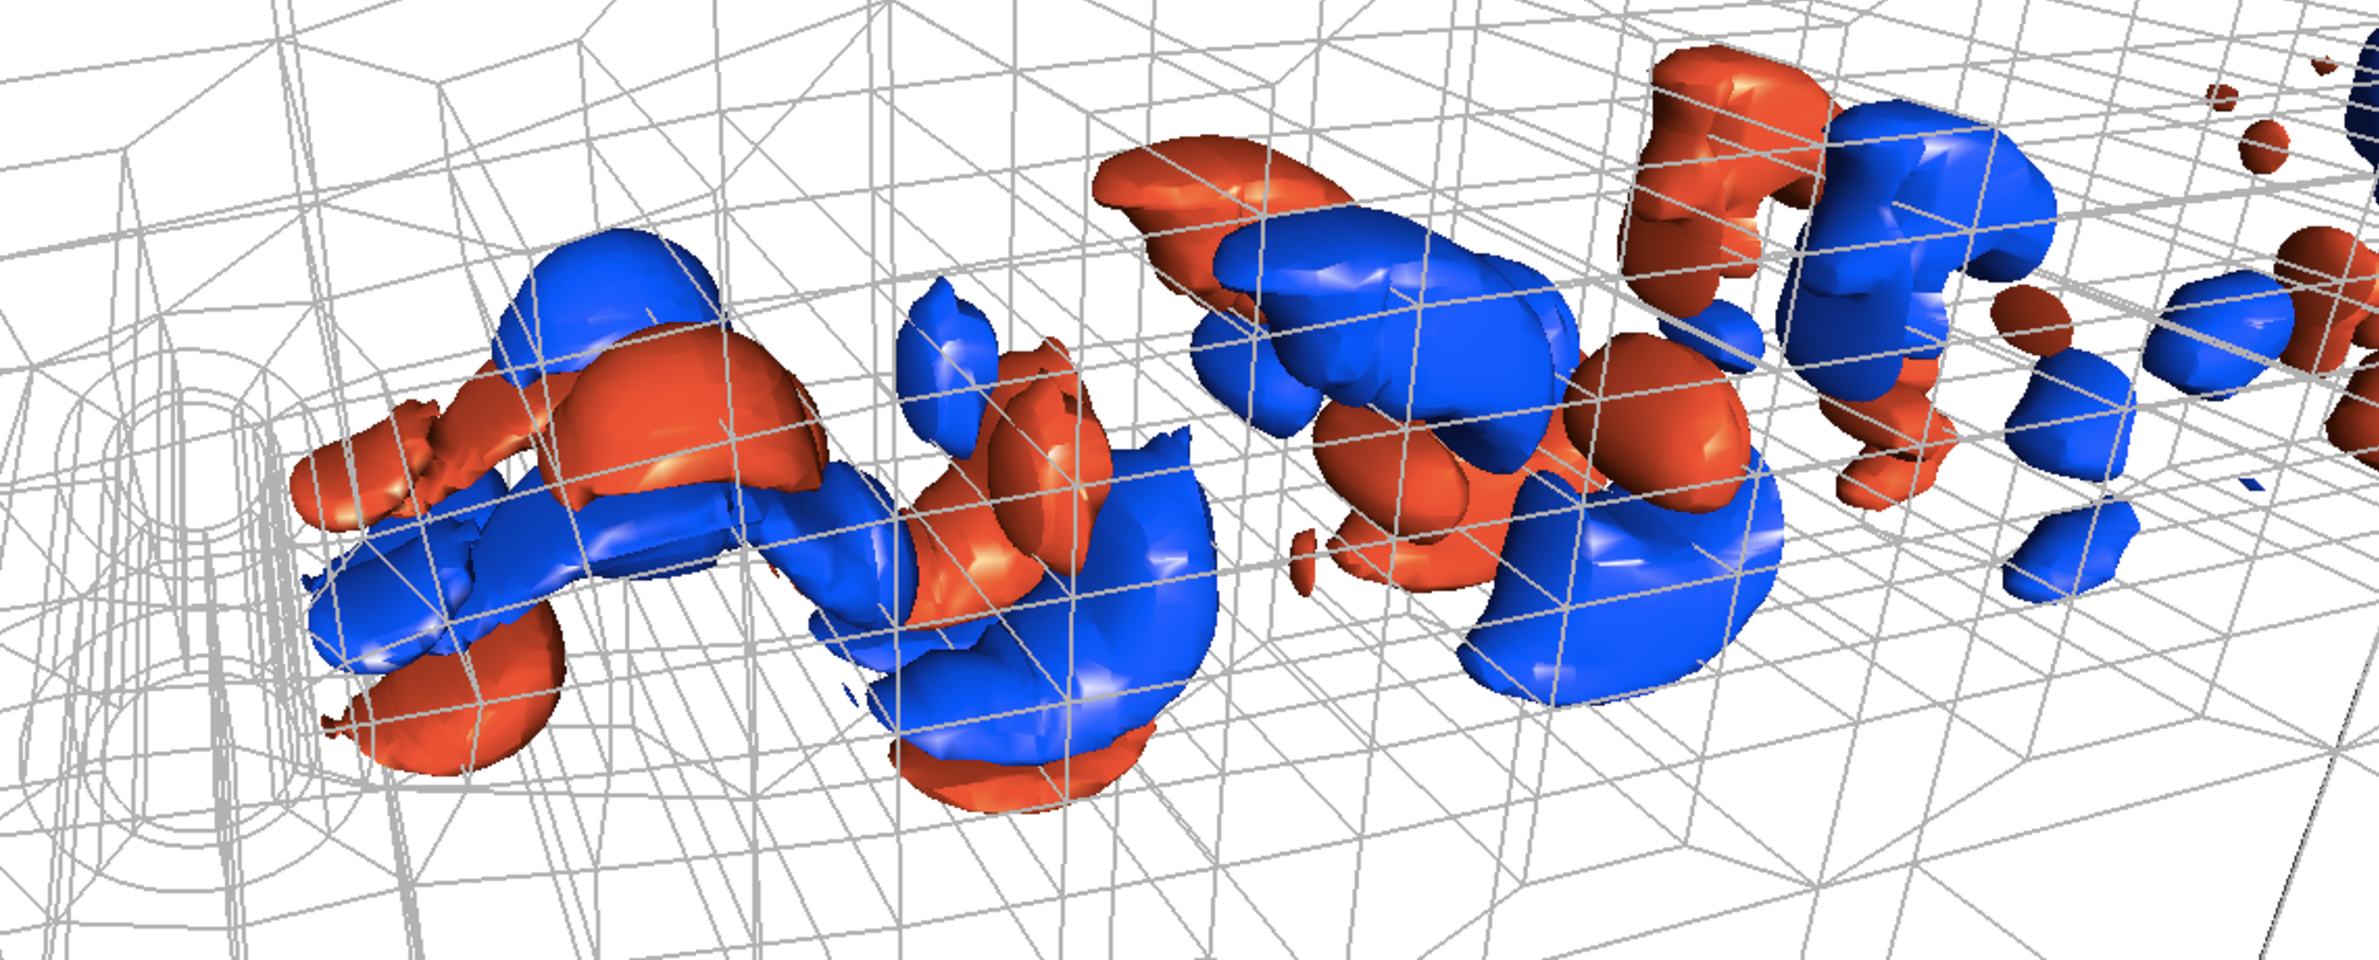
\includegraphics[width=0.7\textwidth]{cyl_flok_mode}
\end{center}
\caption{Leading Floquet mode of the circular cylinder wake at
  $\Rey=188.5$, visualised as isosurfaces of spanwise velocity
  component. (The tool used for visualisation was \texttt{sview}, a
  package also distributed with \Semtex.)}
\label{fig.flok}
\end{figure}


%-----------------------------------------------------------------------------
\subsection{Cross-check: neutral stability of the autonomous limit cycle}

A good cross-check in this case (where the base flow arises as an
autonomous non-linear oscillation) is that in the 2D2C limit, we also
obtain a Floquet multiplier $\mu=1$, as discussed in
\S\,\ref{sec.floquet}.  We could either remake the analysis above with
a very small value of $\beta$, or make a new \Dog\ session file where
the perturbation is 2D2C, like the base flow.  Using the second
approach (session file not detailed), we get this outcome (again based
on a Krylov dimension of 21): {\small
\begin{verbatim}
-- Iteration = 33, H(k+1, k) = 0.713053
EV  Magnitude   Angle       Growth      Frequency   Residual
 0  9.9649e-01  0.0000e+00 -6.8832e-04  0.0000e+00  9.7717e-07
 1  6.3821e-01  0.0000e+00 -8.7842e-02  0.0000e+00  4.2658e-02
..
..
20  1.4306e-01  0.0000e+00 -3.8035e-01  0.0000e+00  6.3940e-01
dog: converged, writing 1 eigenvectors.
\end{verbatim}
}\noindent Again, our estimate is slightly too low, but lies within
0.4\% of the required value.


%%%%%%%%%%%%%%%%%%%%%%%%%%%%%%%%%%%%%%%%%%%%%%%%%%%%%%%%%%%%%%%%%%%%%%%%%%%%%%
\chapter{Optimal growth analysis}
\label{ch.tg}


%=============================================================================
\section{Steady flow in a backward-facing step geometry
\protect\footnote{Input files for this example are supplied in
  \texttt{dog/testcases/Transient/backstep}.}  }
\label{sec.bfsTG}

We will examine optimal transient growth for flow in a backward-facing
step geometry.  Our mesh (shown in figure~\ref{fig.bfsmesh} is the
same as the production mesh $M_1$ used by \citet{bbs08a}.  We will
consider optimal transient growth of 2D2C perturbations at
$\Rey=U_{\max}h/\nu=500$ and with time horizon $\tau=60$, see results
in Table~2 of that reference.  For polynomial order $N=6$,
corresponding to \verb+N_P=7+, they found optimal growth value
$G=62\,661$.

\begin{figure}
\begin{center}
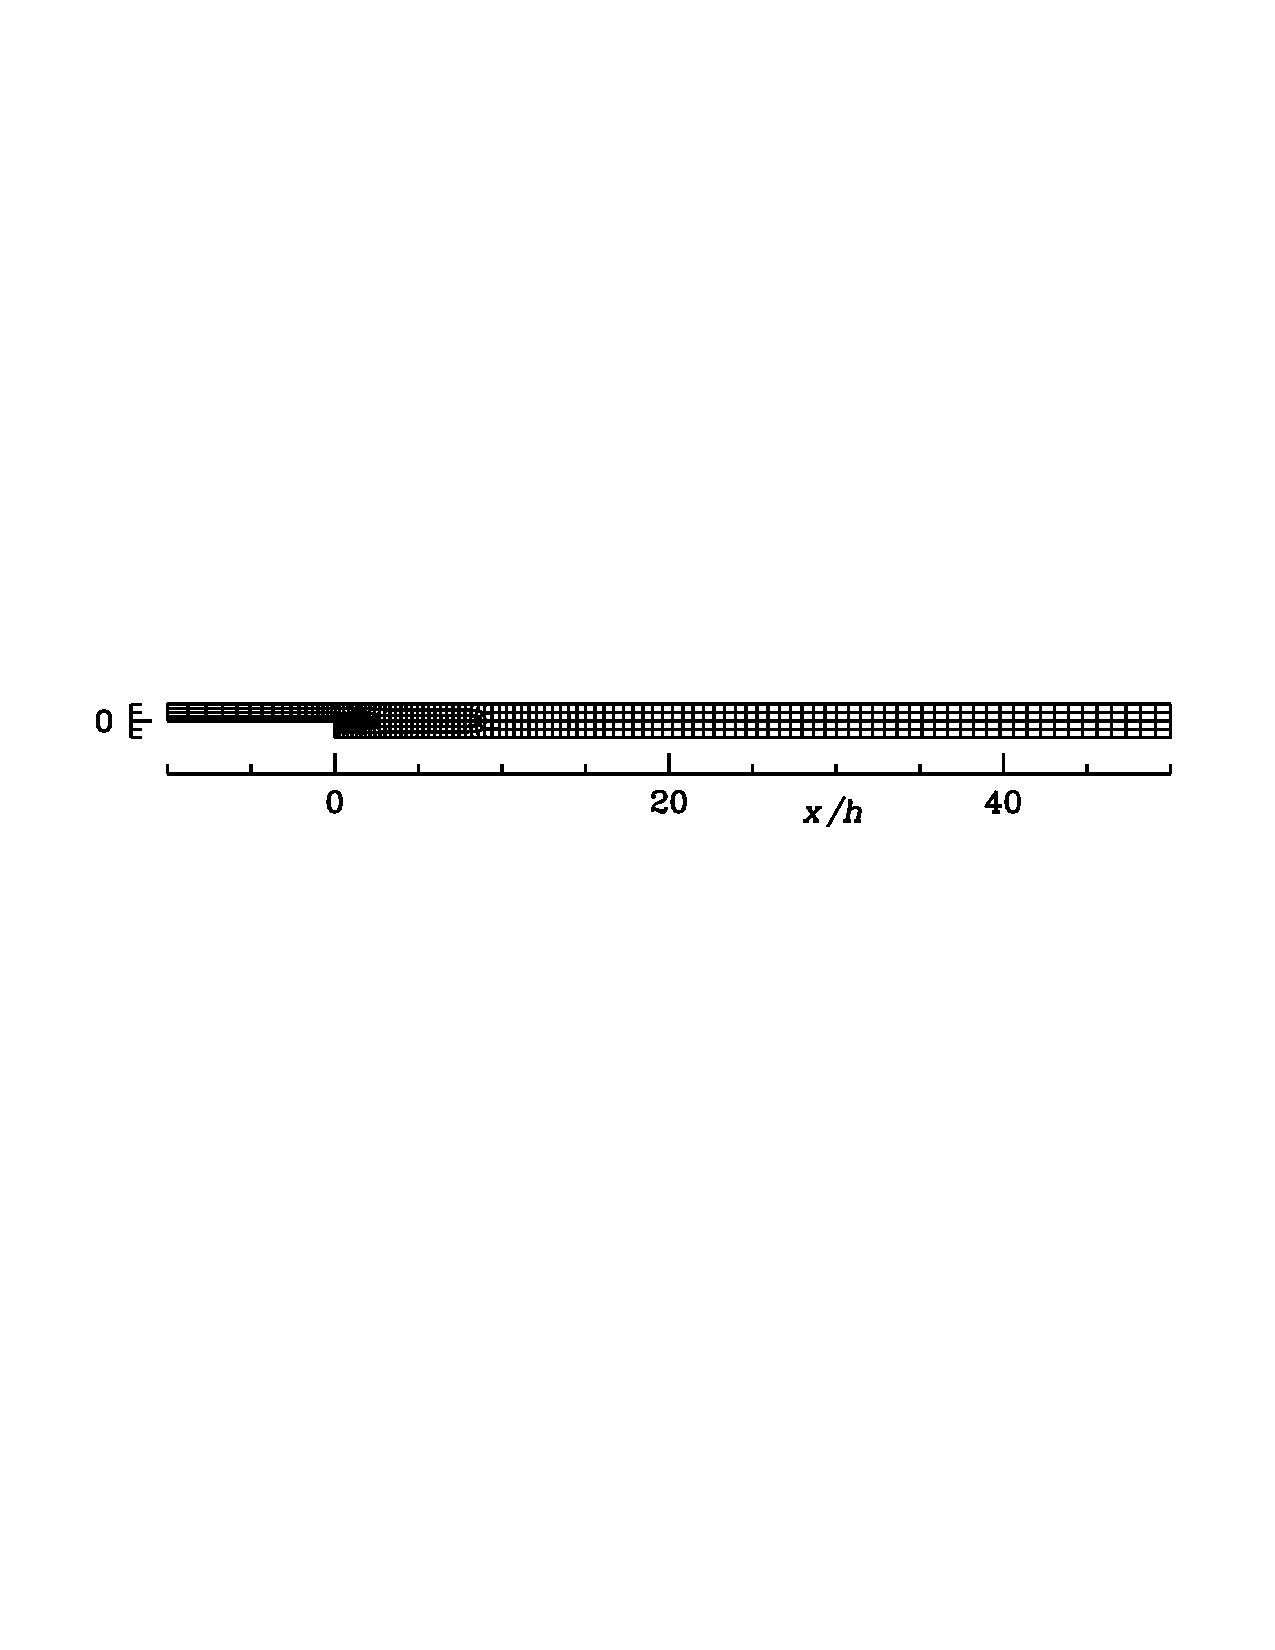
\includegraphics[width=\textwidth]{bfs12mesh}
\end{center}
\caption{Spectral element mesh for the backward-facing step.}
\label{fig.bfsmesh}
\end{figure}

The base flow file is supplied as \verb+bfs12-base+. Below we see a
partial listing.
{\small
\begin{verbatim}
# Backward-facing step
# Li = 10
# Lo = 50
# 563 elements

<FIELDS>
  u  v  p
</FIELDS>

<TOKENS>
  N_TIME  = 2
  N_P     = 7
  T_FINAL = 1450
  D_T     = 0.005
  N_STEP  = int(T_FINAL/D_T)
  Re      = 500
  KINVIS  = 1.0/Re
  IO_CFL  = 25
  IO_HIS  = 10
  IO_FLD  = 1000
</TOKENS>

<HISTORY NUMBER=3>
   1  5	 -0.5  0
   2  15  0    0
   3  30  0    0
</HISTORY>

<GROUPS NUMBER=3>
  1  v  value
  2  w  wall
  3  o  exit
</GROUPS>

<BCS NUMBER=3>
  1  v  3
    <D>  u = 4.0*y*(1-y)  </D>
    <D>  v = 0.0          </D>
    <H>  p                </H>
  2  w  3
    <D>  u = 0.0  </D>
    <D>  v = 0.0  </D>
    <H>  p        </H>
  3  o  3
    <N>  u = 0.0  </N>
    <N>  v = 0.0  </N>
    <D>  p = 0.0  </D>
</BCS>
\end{verbatim}
}
\noindent We will run the base flow for 1450 time units, which is (we
trust) sufficient.

%-----------------------------------------------------------------------------
\subsection{Optimal initial condition}
\label{sec.bfstg}

First, examine the parts of the base flow file that we modify for the
transient growth analysis (this is supplied as file \verb+bfs12+).
{\small
\begin{verbatim}
<FIELDS NUMBER=3>
  u  v  p
</FIELDS>

<TOKENS>
  N_BASE    = 2
  N_SLICE   = 1
  N_TIME    = 2
  N_P       = 7
  T_FINAL   = 60
  D_T       = 0.005
  N_STEP    = int(T_FINAL/D_T)
  Re        = 500
  KINVIS    = 1.0/Re
  IO_CFL    = 25
  IO_HIS    = 10
  IO_FLD    = 1000
</TOKENS>

<SURFACES NUMBER=228>
    1  297  3  <B>  w  </B>
    2  2    2  <B>  w  </B>
   ..
   ..
  228  563  2  <B>  w  </B>
</SURFACES>
\end{verbatim}
}\noindent Note that we have set the time horizon at $\tau=60$ (the
optimal initial condition and growth value we arrive at are dependent
on this parameter).  We have set the boundary conditions to be of wall
type on all \verb+SURFACES+ by the simple expedient of placing them
all in the \verb+w+ (wall) group.
\begin{verbatim}
[mec-aquila]$ ln -s bfs12-base.fld bfs12.bse
[mec-aquila]$ enumerate -O3 bfs12 > bfs12.num
[mec-aquila]$ dog -g -k 4 -n 2 -m 20 -t1e-5 bfs12 > /dev/null &
[mec-aquila]$ tail -f bfs12.evl
\end{verbatim}
\noindent
Note the use of a new command line flag: \verb+dog -g+, requesting a
`growth' computation, and which gives as output the spatial
distribution of optimal initial disturbance.  In fact, we have asked
for two initial disturbances, which are the optimal and first
sub-optimal disturbance \citep[see \S\,4.2.1 and table~5
  of][]{bbs08a}.  If we want the optimal disturbances at the final
time $t=\tau=60$, we would use \verb+dog -s+ (\verb+s+ for `shrink')
instead.  We would get the same results (same $G$ values) in the
\verb+bfs12.evl+ file, but the spatial distributions would be quite
different.

The iteration terminates with
{\small
\begin{verbatim}
-- Iteration = 6, H(k+1, k) = 1025.59
EV  Magnitude   Angle       Growth      Frequency   Residual
 0  6.2661e+04  0.0000e+00  1.8409e-01  0.0000e+00  1.4969e-02
 1  4.7445e+04  0.0000e+00  1.7946e-01  0.0000e+00  2.1796e-02
 2  5.7560e+03  0.0000e+00  1.4430e-01  0.0000e+00  5.1699e+02
 3  5.0410e+03  0.0000e+00  1.4209e-01  0.0000e+00  8.3171e+02
dog: converged, writing 2 eigenvectors.
\end{verbatim}
}\noindent So our value for $G=62\,661$, exactly as expected.  Note
that $G\equiv\texttt{Magnitude}$ (not \verb+Growth+ as you might have
expected), and that the eigenvalues should all be real (since
$\Madj\Mop$ is symmetric).

Since the time horizon for transient growth is a parameter of the
problem, we need to re-run the analysis over a range of $\tau$ values
to find the envelope of growth $G(\tau)$.

%%%%%%%%%%%%%%%%%%%%%%%%%%%%%%%%%%%%%%%%%%%%%%%%%%%%%%%%%%%%%%%%%%%%%%%%%%%%%%
\chapter{Troubleshooting}
\label{sec.trouble}

It is quite common not to be able converge an eigensystem estimate
when first tackling a problem.  Here are some things to consider in
this case:

\begin{enumerate}
\item
Is your base flow up to the job?  Is it (a) well enough resolved
spatially (check vorticity contours) (b) in an asymptotic state,
either steady or periodic (try running it longer)? If the base flow is
meant to be unsteady (\eg periodic) it can be worth making an
animation to check behaviour over a whole cycle, as mesh-related
artifacts can sometimes introduce spurious dynamics \citep[see \eg
  \S\,4.1 of][]{bbs08b}.
\item
Have you used the correct boundary conditions for the base flow and
stability analysis (they are different)?  If you have changed the
boundary conditions while testing, did you re-run \texttt{enumerate}?
\item
How many velocity components are present in your base flow?  If there
are three (i.e.\ there is a $w$ velocity component in the base flow),
you need \verb+N_Z=2+ in your stability analysis session
file\,---\,this allows eigenmodes to have the correct travelling wave
structure in $z$.  Otherwise use \verb+N_Z=1+ or leave it unset (since
\verb+N_Z=1+ is the default)\,---\,this forces eigemodes to be
standing waves in $z$. See the remarks at the end of
\S~\ref{sec.steady}.  If in doubt, it is safe to use \verb+N_Z=2+.
\item
Have you used the same Reynolds number (\verb+KINVIS+) for the base
flow and stability analysis?
\item
If the base flow is time-periodic, do you have enough time-slices for
adequate reconstruction?  Consider using the \verb+BASE_HIST+ section
to output base flow reconstruction history, compare to the equivalent
values achieved in simulating the base flow with \verb+dns+.
\item
Do you have enough spatial resolution? It is easy to change
interpolation order via \verb+N_P+ ($p$-refinement), though often a
better spectral element mesh ($h$-refinement) can be a better solution
at lower computation cost.
\item
Related: are you able to converge an eigenvalue for this problem/mesh
but at a lower Reynolds number?
\item
In a steady stability analysis, the integration time $\tau$ is a
choice made by the analyst.  If it is very different from the
characteristic time ($\lambda^{-1}$) of the problem you're studying,
convergence is unlikely to be achieved.  Consider changing
\verb+N_STEP+: typically it is of the order of a few tens to a few
hundred times \verb+D_T+. It is worth noting that the same value of
\verb+D_T+ is typically appropriate to both the base flow simulation
and the linear analysis.
\item
Examine the convergence history in the \verb+session.evl+ file.  Was
convergence nearly achieved (leading residual came down to of order
say $1\times10^{-4}$ times \verb+MAGNITUDE+ before rising again and
failing)?  Consider relaxing the convergence tolerance to this minimum
level so you can deliver a converged outcome, and examine the flow
structure in \verb+session.eig.0+ to see if that gives any clues (\eg
evidence of under-resolution in a particular location).
\item
So you have managed to obtain a converged eigenpair estimate?  It is
good practice to check that when this is used as a restart
(\verb+.rst+) file for \verb|dog|, the solver rapidly converges to the
same eigenvalue/vector.
\end{enumerate}



%%%%%%%%%%%%%%%%%%%%%%%%%%%%%%%%%%%%%%%%%%%%%%%%%%%%%%%%%%%%%%%%%%%%%%%%%%%%%

\bibliographystyle{dcu} \bibliography{userguide}

%%%%%%%%%%%%%%%%%%%%%%%%%%%%%%%%%%%%%%%%%%%%%%%%%%%%%%%%%%%%%%%%%%%%%%%%%%%%%
\end{document}
